\documentclass[
  reprint,
  amsmath,
  amssymb,
  aps,
  pra,
  nofootinbib,
  superscriptaddress,
  floatfix
]{revtex4-2}
\usepackage[T1]{fontenc}
\usepackage{lmodern}
\usepackage{newunicodechar}
\newunicodechar{’}{'}
\usepackage{graphicx}
\graphicspath{{../../}{}}
\usepackage{capt-of} % \captionof for non-floating figures (used with widetext)
\usepackage{booktabs}
\usepackage{bm}
\usepackage{mathtools}
\usepackage{amsthm}
\usepackage{xcolor}
\usepackage{hyperref}
\hypersetup{hidelinks}

\newcommand{\placeholder}[1]{\textcolor{red!70!black}{\ifmmode\left[#1\right]\else\textsf{[#1]}\fi}}
\newcommand{\tentative}[1]{\textcolor{red!70!black}{#1}}
\newcommand{\structlabel}[1]{\noindent\mbox{\tentative{#1.}}~}
\newcommand{\Oset}{\mathcal{O}}
\newcommand{\Gset}{\mathcal{G}}
\newcommand{\Rset}{\mathcal{R}}
\newcommand{\Sset}{\mathcal{S}}
\newcommand{\Hcal}{\mathcal{H}}
\newcommand{\Bcal}{\mathcal{B}}
\newcommand{\Ocal}{\mathcal{O}}
\newcommand{\Ucal}{\mathcal{U}}
\newcommand{\Jcal}{\mathcal{J}}
\newcommand{\Pcal}{\mathcal{P}}
\newcommand{\Dcal}{\mathcal{D}}
\newcommand{\Wcal}{\mathcal{W}}
\newcommand{\dd}{\mathrm{d}}
\newcommand{\ii}{\mathrm{i}}
\newcommand{\ee}{\mathrm{e}}
\newcommand{\TR}{\mathrm{TR}}
\newcommand{\ex}{\mathrm{ex}}
\newcommand{\ctrl}{\mathrm{ctrl}}
\newcommand{\stat}{\mathrm{stat}}
\newcommand{\dyn}{\mathrm{dyn}}
\newcommand{\drv}{\mathrm{drv}}
\newcommand{\obs}{\mathrm{obs}}
\newcommand{\stay}{\mathrm{stay}}
\newcommand{\app}{\mathrm{append}}
\newcommand{\ablate}{\mathrm{ablate}}
\newcommand{\Var}{\operatorname{Var}}
\newcommand{\Tr}{\operatorname{Tr}}
\newcommand{\Top}{\operatorname{Top}}
\newcommand{\argminp}{\mathop{\mathrm{arg\,min}}}
\newcommand{\argmaxp}{\mathop{\mathrm{arg\,max}}}
\newcommand{\proj}{\mathrm{proj}}
\newcommand{\diag}{\mathrm{diag}}
\newcommand{\CVaR}{\operatorname{CVaR}}
\newcommand{\softmax}{\operatorname{softmax}}
\newcommand{\hh}{\mathrm{HH}}
\newcommand{\phmax}{n_{\mathrm{ph,max}}}
\newcommand{\twq}{\mathrm{2Q}}
\newcommand{\eps}{\varepsilon}
\newcommand{\ket}[1]{|#1\rangle}
\newcommand{\bra}[1]{\langle #1|}
\newcommand{\braket}[2]{\langle #1|#2\rangle}
\newcommand{\expval}[1]{\langle #1\rangle}
\newcommand{\metrichead}[1]{\makebox[0.061\textwidth][c]{#1}}
\newcommand{\archmetrichead}[1]{\makebox[0.040\textwidth][c]{#1}}
\newcommand{\inlinetablecaption}[2]{%
  \par\addvspace{1.6ex}%
  \captionof{table}{#2\label{#1}}%
  \par\addvspace{0.8ex}%
}
\newenvironment{schurlemma}[1][]
{\par\medskip\noindent\textbf{Lemma}\if\relax\detokenize{#1}\relax\else\ (#1)\fi.\space\itshape}
{\par\medskip}
\newenvironment{schurassumption}[1][]
{\par\medskip\noindent\textbf{Assumption}\if\relax\detokenize{#1}\relax\else\ (#1)\fi.\space}
{\par\medskip}
\newenvironment{schurtheorem}[1][]
{\par\medskip\noindent\textbf{Theorem}\if\relax\detokenize{#1}\relax\else\ (#1)\fi.\space\itshape}
{\par\medskip}
\newenvironment{schurremark}[1][]
{\par\medskip\noindent\textbf{Remark}\if\relax\detokenize{#1}\relax\else\ (#1)\fi.\space}
{\par\medskip}


\begin{document}

\makeatletter
\def\bibsection{\section*{\refname}\@nobreaktrue}
\makeatother

\title{Geometric and Resource-Aware Adaptive Ansatz Construction Applied to the Hubbard--Holstein Dimer}

\author{Jake Strobel}
\author{Jacopo Simoni}
\author{Gabriele Riva}
\author{Yuan Ping}
\affiliation{University of Wisconsin--Madison}

\date{\today}

% BEGIN_EDITORIAL_FRAMING_NOTES_20260718
% High-level paper framing to preserve during the next prose pass:
% - Introduce SNAKE as a highly accurate, hardware-aware ADAPT-VQE-style
%   algorithm whose staged shortlisting increasingly approximates a
%   supported Fubini--Study joint second-order response model.
% - State that generators are admitted using predicted energy gain together
%   with hardware circuit-cost weights.
% - Headline the demonstrated outcome as substantially lower energy error,
%   two-qubit gate count, two-qubit depth, and total circuit depth, together
%   with increased logical estimator-query burden. Add one-qubit gate claims
%   once N1q is summarized consistently from the canonical sidecars.
% - Frame recoverability pruning as the mechanism intended to offset part of
%   the added S_alg burden. Its quantitative effect remains pending the active
%   prune-enabled run.
% - Frame beam search as a complementary mechanism for depth-limited settings:
%   retaining several promising branches can locate shallower constructions
%   when qubit support is available and compiled depth is the bottleneck.
% - Place support projection in the mathematical core; reserve explicit
%   Fubini--Study whitening for the coordinate-sensitive accepted refit.
% - Add prefix-level plots of same-cutoff error versus N2q, D_c, and S_alg.
% - The benchmark-configuration table already records the variable trust-region
%   policy in its "Trust update" row; preserve that row in subsequent edits.
% END_EDITORIAL_FRAMING_NOTES_20260718
\begin{abstract}
Near-term ground-state quantum simulation requires adaptive ansätze that achieve target accuracy while minimizing circuit depth and quantum-estimator overhead. ADAPT-VQE constructs ansätze by iteratively selecting generators from an operator pool; however, its generator-selection mechanism remains sensitive to local gradient plateaus, generator parameterization, and state-tangent redundancy while remaining agnostic to generator-specific hardware costs. We introduce the Selection-Novel ADAPT Kost Evaluator (SNAKE), whose central contribution is a staged generator-scoring subroutine that progressively escalates local geometric response modeling through three phases before admitting a hardware-cost-weighted candidate according to a Schur-reduced Fubini--Study pullback trust-region response model. This common geometric framework further supports pullback-coordinate whitening for coordinate-sensitive accepted refits, Lowerre-style beam search, and pullback trust-region response models for Tetris-style batch admission and generator pruning. We benchmark SNAKE against append-only ADAPT-VQE and Geo-ADAPT on the Hubbard, spin-boson/Rabi, Bose--Hubbard, and Hubbard--Holstein models using matched qubit encodings, operator pools, and inner-optimization protocols. At the fixed Hubbard--Holstein accuracy target $E_T=2\times10^{-4}$, SNAKE reaches the target in all six interaction regimes, whereas intact-macro Geo-ADAPT and append-only ADAPT reach it in one and two regimes, respectively, and projected-singleton append-only ADAPT reaches it in five. Summed over the five regimes reached by both SNAKE and the projected-singleton append-only comparator, SNAKE reduces $N_{2q}$, $D_{2q}$, total circuit depth, and logical estimator work by $32\%$, $42\%$, $21\%$, and $82\%$, respectively. These results demonstrate that staged geometric response modeling can attain prescribed ground-state accuracy with substantially lower circuit and measurement resources.


\end{abstract}

\maketitle







\section{Introduction}

Significant interest has been given to quantum computing in recent years. One motivation is that quantum processor units (QPU) can offer computational speedups. Such speed-ups include physics simulation like finding the ground-state ansatz of a given Hamiltonian \cite{Lloyd1996,AspuruGuzik2005}. The scope of available simulation problems is limited by QPU recourse constraints, where circuit-depth, entangling gate-count, and measurement overhead generally monotonically increase measurement error \cite{Preskill2018NISQ,Cerezo2021VQA,Huggins2021Measurements}. This current QPU state is classified as the noisy intermediate-scale quantum (NISQ) era, and many classes of algorithms have been devloped specifically to address these bottlenecks. One such class are Adaptive derivative-assembled pseudo-Trotter variational quantum eigensolvers (ADAPT-VQE),  which iteratively recursively construct circuits by appending gates according from a pre-defined operator pool based on an energy-gradient selection rule. Although ADAPT-VQE has found significant success on small Fermionic systems, with limited applications to Fermionic and Bosonic models (CITE), ADAPT-VQE can still fail to reach acceptable accuracies of ground-state preparation due to forbidding circuit-depths, prohibitive measurement overhead, insufficiently-expressive operator pools, and-or energy-plateaus due to poorly conditioned variational coordinate landscapes. \cite{Grimsley2019,Tang2021,Yordanov2021,Feniou2023,Ramoa2025HessianRecycling,Ikhtiarudin2025ShotEfficient}.  Thus ansatz construction through operator selection becomes the dominant lever for NISQ ground-state ansats preparation. We present SNAKE/SCORE/BS, as a highly-accurate, recourse-aware operator-selection subroutine of ADAPT-VQE.


\subsubsection{Modeled problem}
To our knowledge, no ADAPT-VQE method has been applied to condensed-matter many-body fermion--phonon Hamiltonians such as the Hubbard--Holstein model \cite{Macridin2018,Li2023,Denner2023,Majland2024vADAPT}. Converse to mixed system electron-phonon models, electronic-structure applications of ADAPT-VQE can draw on a mature literature of unitary coupled cluster singles and doubles (UCCSD) excitation operators \cite{Romero2018UCC,Grimsley2019}. There is not a comparably established operator-pool construction for mixed fermion--phonon condensed-matter models. This creates the problem of operator pool definition, in addition to the problem of operator selection. In the Hubbard--Holstein setting, such a pool must span electronic correlation, phononic lattice response, and coupled electron--phonon dressing, and the encoded ansatz requires fermion--boson sector-entangling gates under a finite phonon-mode truncation \cite{Hubbard1963,Holstein1959a,Holstein1959b}. We define operator pools in section~\ref{subsec:hh_physical_operator_lanes} and <CITE HH POOL AND SPIN-BOSON/HUBBARD/BOSE-HUBBARD>. We focus results on the Hubbard--Holstein model under six interaction-strength regimes and compare SNAKE against append-only ADAPT-VQE, and Geo-ADAPT, using transpiled circuit resources and estimator queries required to reach a shared energy-error target.


The Hubbard--Holstein model is given by
\begin{align}
H
&=-t\sum_{\langle i,j\rangle,\sigma}
(c_{i\sigma}^{\dagger}c_{j\sigma}+c_{j\sigma}^{\dagger}c_{i\sigma})
+U\sum_i n_{i\uparrow}n_{i\downarrow}
\nonumber\\
&\quad+\omega_0\sum_i b_i^\dagger b_i
+g\sum_i(b_i^\dagger+b_i)(n_i-\bar n).
\label{eq:hubbard_holstein_static}
\end{align}
Here \(c_{i\sigma}\) and \(b_i\) correspond to fermionic and bosonic annihilation operators, respectively, acting on site $i$, with creation given by $\dagger$; $\sigma \in\{\uparrow, \downarrow\}$ denotes particle spin;
\(n_{i\sigma}, n_i\) are the spin-resolved and total fermionic number operators, respectively; \(\bar n=N_e/L\) is the mean fermion filling for fixed electron number \(N_e\) and lattice size \(L\). Our results use open boundary conditions with half-filling. Here \(t\) is the nearest-neighbor electronic hopping amplitude, \(U\) is the onsite Hubbard interaction, \(\omega_0\) is the phonon frequency, \(g\) is the local electron--phonon coupling, and \(\langle i,j\rangle\) denotes nearest-neighbor lattice sites.
In the joint decoupling limit $g\to0$ and $\omega_0\to0$, the electronic sector reduces to the Hubbard Hamiltonian, up to a decoupled zero-frequency phonon register. We use Jordan--Wigner and binary encoding for Eq.~\eqref{eq:hubbard_holstein_static} and the operator-pool generators in Appendix~\ref{app:lane_shortlisting}, with fixed blocked qubit registers.


\subsubsection{Current status}
ADAPT-VQE recursively and iteratively builds a parameterized circuit by adding the operator which maximizes the states local energy gradient \cite{Grimsley2019,Tang2021,Yordanov2021}. First define an initial reference state $\ket{\psi_{\rm{ref}}}$, taken as the Hartree-Fock slater determinant tensored with the phonon vacuum at a chosen phonon mode cutoff. We denote this as  \(\ket{\psi_{\mathrm{ref}}}=\ket{\mathrm{HF}}\otimes\ket{0_1\,0_2\,\cdots\,0_{\mathrm{M}}}\), where \(M\) is the number of retained phononic modes. With the addition of a defined operator pool $\mathcal G$, and an encoded Hamiltonian $H$, the ADAPT-VQE algorithm is sufficiently defined. Specifically, the ansatz update rule is given by, 
\begin{equation*}
U_{k+1}(\boldsymbol{\theta}_{k})=e^{-i\theta_{n_k} A_k^\star}U_k(\boldsymbol{\theta}_{k-1}).
% source label: eq:adapt_append_update
\end{equation*}
where $U(\boldsymbol{\theta})$ is the ansatz circuit parameterized by vector  $\boldsymbol{\theta}=(\theta_1,\ldots,\theta_n)$ and composed of exponentiated Hermitian generators $A \in \mathcal G$ which generate unitaries through \(e^{-i\theta A}\). The selection of a generator $A^*$ follows from 
\begin{equation}
A_k^\star=\arg\max_{A\in\mathcal G}
\left|
\left.
\partial_{\theta_{n_k}}E\!\left(e^{-i\theta_{n_k} A}U_k(\boldsymbol{\theta}_{k-1})\ket{\psi_{\mathrm{ref}}}\right)
\right|_{\theta_{n_k}=0}
\right|\,,
\label{eq:adapt_append_gradient}
\end{equation}
where $E(\boldsymbol{\cdot})$ is the expectation value of the Hamiltonian on the trial wave function, $\ket{\psi(\boldsymbol{\theta})}:=U(\boldsymbol{\theta})\ket{\psi_{\rm ref}}$. Here and below, a superscript $\star$ marks the selected or optimized extremizer. Between each ansatz update iteration, known as the outer loop, an inner loop occurs, which entails a classical optimizer varying $\boldsymbol{\theta}$  to exploit the Raleigh--Ritz criterion \cite{Peruzzo2014,McClean2016,Kandala2017}. Namely, 
\begin{equation}
\label{eq:theta_opt}
\boldsymbol{\theta}^\star=\arg\min_{\boldsymbol{\theta}}E(\boldsymbol{\theta})\,,
\end{equation}
where \begin{equation}
E(\boldsymbol{\theta})=
\bra{\psi_{\rm ref}}U^\dagger(\boldsymbol{\theta})HU(\boldsymbol{\theta})\ket{\psi_{\rm ref}}.
\label{eq:rayleigh_static}
\end{equation}
Different inner optimization methods exist, such as direct search or gradient-based optimization procedures \cite{BonetMonroig2023Optimizer,Singh2023Optimizers,Gacon2021QNSPSA}. 

Numerous ADAPT variants modify the outer-loop generator-selection rule. CEO-ADAPT uses coupled-exchange operator sequencing \cite{Ramoa2025}, whereas Overlap-ADAPT incorporates tangent-direction information into the append criterion \cite{Feniou2023}. Other methods exploit second-order derivative information to improve convergence \cite{Grimsley2023ADAPT} or recycle Hessian information to warm-start successive refits \cite{Ramoa2025HessianRecycling}. Contemporaneous with this work, Geo-ADAPT-VQE ranks candidates according to their predicted Fubini--Study state displacement by equipping the candidate pool with the pullback Gram matrix and optionally allowing generator insertion rather than append-only growth \cite{Sohail2026GeoADAPT}. Prune ADAPT removes previously selected generators using amplitude- and history-based criteria \cite{Vaquero2025PrunedADAPT}.

\subsubsection{Limitations with current approaches}
Despite these advances, current adaptive strategies leave several unresolved issues. Standard ADAPT relies on first-order energy gradients to select generators \cite{Grimsley2019,Tang2021,Yordanov2021} and therefore can result in myopic generator selection thereby increasing circuit depths compared to a curvature-aware method \cite{Feniou2023,Grimsley2023ADAPT}. Geo-ADAPT computes the Gram matrix of the state-space tangent vectors generated by the full operator pool, which is the pullback of the Fubini--Study metric to the pool-parameter coordinates. It then multiplies the energy-gradient covector by the inverse of this Gram matrix to obtain the coefficient vector of the Riemannian gradient in the basis of pool-induced state tangents, and selects the generator corresponding to the largest-magnitude coefficient. This metric relies on matrix inversion, which can become ill-conditioned or rank deficient when the induced tangent directions are redundant or linearly dependent \cite{Sohail2026GeoADAPT}. Furthermore, the full Gram matrix taken over the candidate operator pool scales as $\mathcal{O}(|\mathcal{G}|^2)$, which may present a measurement bottleneck.\cite{Ramoa2025HessianRecycling,Ikhtiarudin2025ShotEfficient}. 
\noindent
The initial motivation of this work resulted from the finding that standard ADAPT-VQE methods plateaued on the Hubbard--Holstein model, and after investigation of alternative NISQ-friendly algorithms, there remained two practical shortcomings. First, absent a cost penalty, candidate operators with marginally different gradient advantages can be treated as equally desirable despite arbitrarily large differences in two-qubit gate, routing, or measurement burden. Second, existing selection algorithms do not explicitly estimate the candidate's energy gain after the current ansatz responds through local reoptimization. This latter motivation resulted in a second-order Schur treatment that enabled the reformulations of TETRIS-ADAPT style selection which appends multiple operators at once, an energy model for Prune-ADAPT, and an objective for Lowerre style beam search.




%
\subsubsection{\textsc{SNAKE}: geometric and resource-aware ansatz growth}
We present \textsc{SNAKE} as an ADAPT-VQE subroutine which modifies the generator selection criterion of the outer ADAPT loop. At the top-down level, SNAKE relies on a trust-region confined second-order Taylor model that couples candidate generators to the existing ansatz ... \textcolor{red}{will return here after updating methods section}

incorporating a Schur-reduced response of candiate-generator-ansatz coupling to predict the Schur
confined to a state-displacement trust-region where the candidate generators 

\textsc{SNAKE} limits parameter-coordinate sensitivity of candidate operators by evaluating generator-induced state-space tangents using a regularized Fubini--Study metric \cite{Sohail2026GeoADAPT}. \textsc{SNAKE} then augments the energy-gradient objective of Eq.~\eqref{eq:adapt_append_gradient} with a second-order Taylor model, and constrains the allowed predicted candidate-induced variational state displacement to a geometric trust region \cite{Nocedal2006TrustRegion}. Phase III jointly optimizes the candidate amplitude and the response of the current ansatz within this trust region; the resulting joint displacement supplies the final ranking and trust-radius calibration.

Candidate operators are then ordered by predicted energy gain per resource cost, where costs
are determined by graph-aware estimates of two-qubit depth, CNOT gate count, compiled circuit depth, required basis rotations, and grouped-measurement shot demand \cite{Verteletskyi2020CliqueCover,Yen2020CompatibleMeasurements,Ikhtiarudin2025ShotEfficient}.
The ordered list of top-ranked candidate operators may be admitted jointly, conditional on nonredundant combined operator-induced state-tangents and predicted additive energy descent after variational refit. We call this process batching.

Furthermore, among the score-ordered proposals, \textsc{SNAKE} may
instantiate leading singleton or batch proposals as parallel circuit branches
using a Lowerre-style beam search \cite{Lowerre1976Beam}. Branch retention is
determined by realized energy gain per added circuit cost.


To reduce unnecessary circuit costs, \textsc{SNAKE} permits ablation of existing circuit generators whose variational directions have become locally redundant within the current ansatz. Specifically, the same second-order local Taylor Schur model with a regularized Fubini--Study metric is used to predict the ansatz's ability to recover the pre-ablation state vector and final energy after removing the generator. An ablated generator decision is preserved if the energy detriment is negligible compared to the resulting savings in circuit costs \cite{Vaquero2025PrunedADAPT}. Conversely, if the modeled ablation prediction is wrong and the realized ablation does not pass a refitted energy per cost threshold, the ablation decision is reversed and the generator is placed on cool-down.

Finally, unlike conventional append-only ADAPT-VQE, \textsc{SNAKE} allows for the insertion of generators within the ansatz circuit. This allows the algorithm to search over the entire circuit structure. \textsc{SNAKE} then ranks these operator--position pairs over an energy-error and hardware-cost Pareto surface.

\textsc{SNAKE} combats the increased measurement overhead of second-order gradient-based generator scoring by using a staged scoring procedure that iteratively restricts the operator--position record set between phases. Each phase reuses the prior phase's measurements while augmenting the record-ordering function with higher-order energy models and geometric information. The resulting phase restriction retains the top-scored records before the next, more expensive phase is evaluated; see Fig.~\ref{fig:static_adapt_selector_flow}.

The record set passed from phase to phase is additionally partitioned according to each operator's inferred physical consequence. In the Hubbard--Holstein case, physically motivated operators define six lanes: UCCSD, electron current/hopping, phonon cloud/displacement, phonon-squeeze relaxation, dressed phonon correlation, and Hamiltonian variational ansatz blocks. This lane partition permits a more aggressive shortlisting policy between phases while preserving competition among distinct physical response channels.


We refer to this staged, geometry-aware, and resource-aware adaptive selector as \textsc{SNAKE}.
%
\section{Staged generator-position ranking}
\label{sec:static_method}
%
\begin{figure*}[t]
\centering
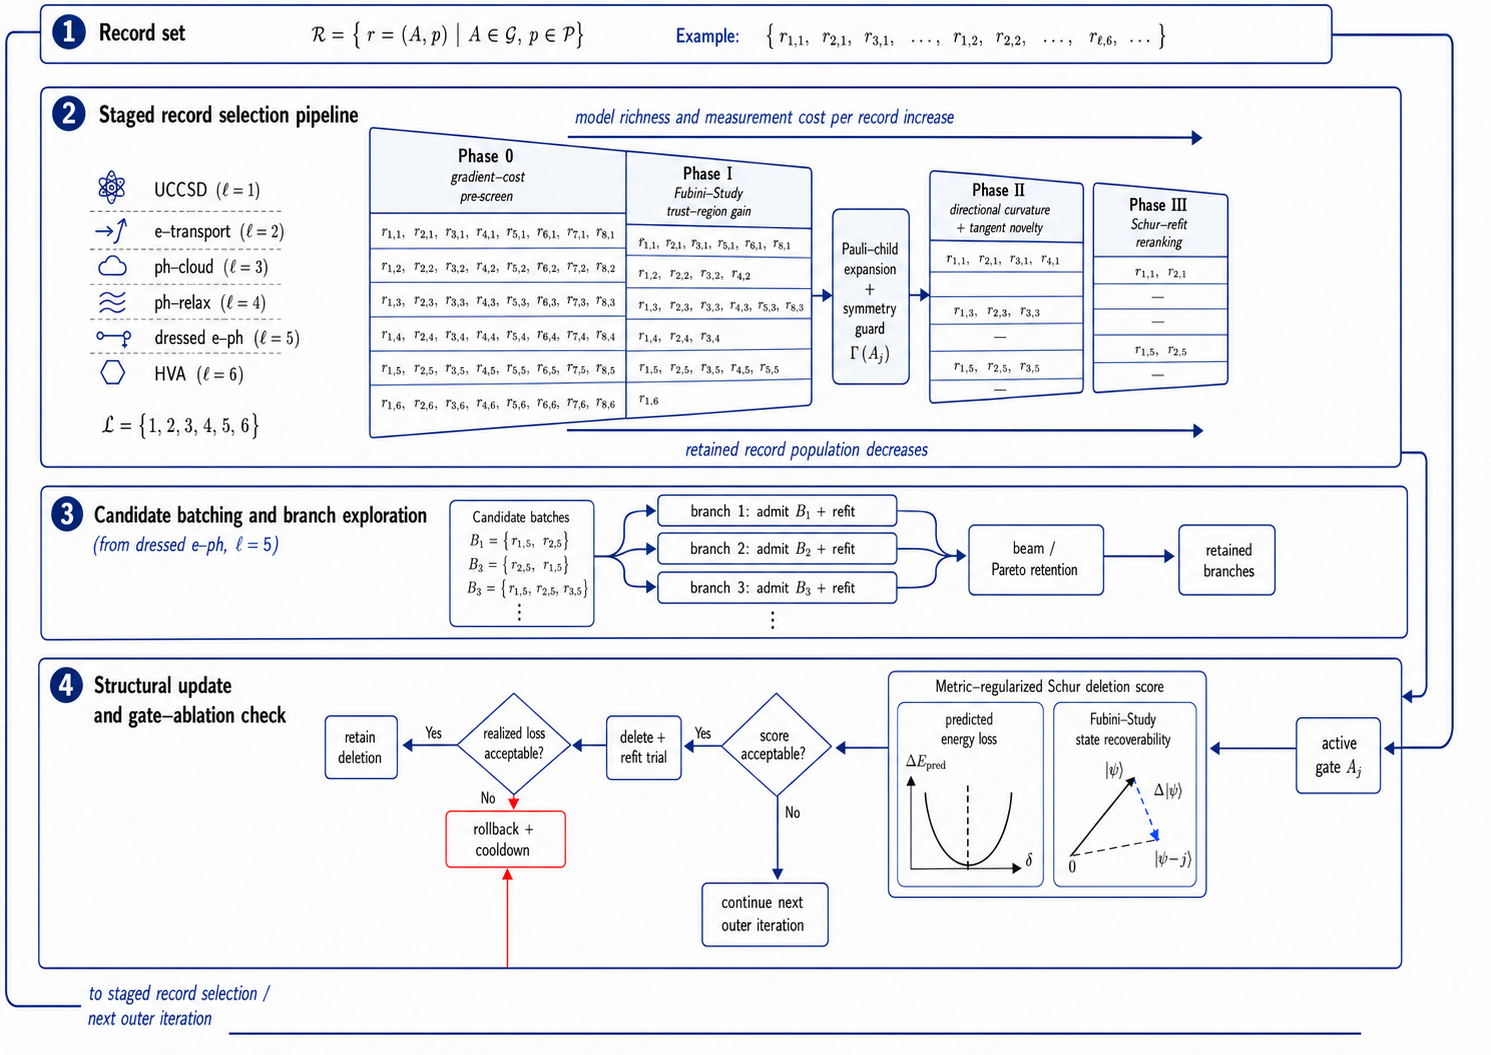
\includegraphics[width=0.97\textwidth]{figures/snake_staged_record_selection_ablation_flow_20260710.png}
\caption{SNAKE ADAPT ansatz-construction flow. (a) Generator--position records
are restricted through staged, lane-protected scoring, Pauli-child expansion
and symmetry screening, batch proposal, and beam/Pareto retention. (b) Retained
branches undergo metric-regularized Schur deletion nomination, explicit
delete--refit validation, rollback and cooldown on rejection, and continuation
to the next outer iteration.}
\label{fig:static_adapt_selector_flow}
\end{figure*}

To prevent excess measurement burden resulting from higher-order modeling, SNAKE relies on a staged three-phase restriction of the candidate operator set. Each phase relies on previously attained measurements, and incorporates higher order modeling but on a smaller candidate pool. This helps shortlist candidates in accordance with predictive confidence while avoiding paying a full measurement burden.

We enable an additional degree of freedom by allowing SNAKE to insert operators at any position within the ordered generator unitary $U(\boldsymbol{\theta})$. This couples the candidate generator set with available circuit insertion positions. Let \(p\in\mathcal P_k\) denote an admissible insertion position and \(A\in\mathcal G\) an available generator. Denote a candidate generator--position record as
\[
r=(A,p),
\]
which is an element of the candidate record set,
\begin{equation}
\mathcal R_k=\mathcal G\times\Pcal_k .
\label{record_set}
\end{equation}
We know define the SNAKE subroutine at the level of record-set restriction. 
At fixed outer iteration \(k\), SNAKE applies two phases which restrict the candidate record set before final admission of a single record. Let $\mathcal R_k$ be the initialized available set which becomes shortlisted to become $\mathcal R^{(1)}$, which inturn becomes shortlisted twice more so that $|\mathcal{R}_k|<|\mathcal{R}^{(1)}|<|\mathcal{R}^{(2)}|<|\mathcal{R}^{(3)}|$ until the top-scored record from $\mathcal{R}^{(3)}$ is admitted to the ansatz. The set restriction is based on retaining the top-valued records, where valuation follows a scalar-valued "scoring" function  $S: r\to \mathbb R$, which allows for the ordering of records $r$ by $\mathbb R$ within $\mathcal{R}^{(t)}$, for $t\in\{1,2,3\}$. Briefly, the function has form $S(r)=\frac{\Delta E(r)}{K(r)}$, where $\Delta E(r)$ is the predicted energy drop from $r$ and $K(r)$ is the records associated circuit cost. See Sec.~(\ref{subsec:cost_weighted_record_ranking}) for details. 

One difference occurs between the set-restriction of $\mathcal{R}_k \to \mathcal R^{(2)}$ compared to $\mathcal{R}^{(2)}\to \mathcal{R}^{(3)}$. Specifically, for $\mathcal{R}_k \to \mathcal R^{(2)}$, operators are classified into physical response channels which enables a partitioning of the record sets $\mathcal{R}^{(1)}$ and $ \mathcal R^{(2)}$. We present such a partition in order to allow for more aggressive shortlisting without deleting an entire physical response channel, where preservation follows by biasing the retainment of records classified under distinct physical channels. Conversely, after the record set restriction which produces $\mathcal R^{(2)}$, the record generators $A\in\mathcal R^{(2)}$, which are conventionally Pauli-polynomials, are decomposed into individual Pauli-words which pose as candidates for admission. The Pauli-word child set is then de-duplicated and exposed to particle-number symmetry guards; See section~\ref{subsec:proposal_refinement_update} for specific Pauli-children details, and see Appendix~\ref{app:lane_shortlisting} for the specific physical response lane definitions and set-partition formalism. 

Explicitly, the record set takes the chained form of

\(\mathcal R_k
\xrightarrow[\text{lane-wise}]{\operatorname{Top}_N{(r\in\mathcal R \mid S^{(1)})}}
\mathcal R^{(1)}
\xrightarrow[\text{lane-wise}]{\operatorname{Top}_N{(r\in\mathcal R^{(1)} \mid S^{(2)})}}
\mathcal R^{(2)}
\xrightarrow[\text{De-duped \& Symm. Guard}]{\operatorname{Pauli-Children}}
\mathcal R^{(3)}
\xrightarrow[\text{insert single or batch}]{\operatorname{Top}_N{(r^*\in\mathcal R^{(3)} \mid S^{(3)})}}
U(\boldsymbol \theta) \oplus r^*.\)

 where $\operatorname{Top}_N{(r\in\mathcal R^{(t)} \mid S^{(t)})}$ denotes retainment of the top $N$ records in $\mathcal R^{(t)}$ under a set ordering given by $S^{(t)}$. Here $\text{lane-wise}$ denotes that the physical response lane partition of the record set is active which influences the set restriction. The text, $\text{De-duped \& Symm. Guard}$ indicates the de-duplication and symmetry guard constraints applied to the Pauli-child record set,  and $\text{insert single or batch}$ denotes a single admission policy or a batched admission policy.

 We now present the energy model $\Delta E$ used in the set-restriction ordering function $S=\frac {\Delta E(r)} {K(r)}$, followed by a section defining the components of $K(r)$ in Sec.~(\ref{subsec:cost_weighted_record_ranking}).

\section{Candidate scoring}
\label{subsec:candidate_energy_models}
%
We present the energy model used in the three-iterated record set restriction subroutine. The score function $S^{(3)}$ evaluates records $r\in\mathcal R^{(3)}$ using a local quadratic model which couples the candidate record to the ansatz. The $\mathcal R^{(2)}$ score function $S^{(2)}$ then assume no-coupling and becomes the 1-D quadratic model. Finally, the initial restriction of $\mathcal R_k \to \mathcal R^{(1)}$ taken by top records ordered by $S^{(1)}$, assumes a linear first order model, and thus is the restriction of no coupling nor second order energy curvature. We mow present this top-down model.
\paragraph*{Coupled local quadratic model.}
%
 Let \(\alpha\) denote the candidate coordinate of the compiled generator $A \mapsto e^{i\alpha A}$, and let $\delta \boldsymbol{\theta}$ denote the predicted ansatz coordinate response after admission. That is, we are modeling $U_k(\delta \boldsymbol{\theta})\oplus e^{i\alpha^* A}\approx U_{k+1}(\boldsymbol{\theta}^*)$. This motivates a model of the form
\begin{equation}
E(\alpha,\delta\boldsymbol\theta)
\approx
E_0+g(r)\alpha
+\frac12
\begin{pmatrix}
\alpha\\
\delta\boldsymbol\theta
\end{pmatrix}^{\!\top}
\begin{pmatrix}
H_{rr} & H_{r\theta}\\
H_{\theta r} & H_{\theta\theta}
\end{pmatrix}
\begin{pmatrix}
\alpha\\
\delta\boldsymbol\theta
\end{pmatrix},
\label{eq:local_quadratic}
\end{equation}
where \(E_0=E(U_k(\boldsymbol\theta_k^\star))\) and the first-order derivatives with respect to the active ansatz coordinates vanish by stationarity. The scalar \(g(r)\) is the
signed candidate-direction derivative, and the four Hessian blocks $H_{uv}$ describe
candidate curvature ($rr$), candidate--ansatz coupling ($r\theta$), and active-ansatz response ($\theta \theta$).
The active-coordinate linear term vanishes at the optimized iterate. Their position-resolved evaluations are given below.

Collect the physical joint displacement as
\begin{equation*}
\mathbf z=
\begin{pmatrix}
\alpha\\
\delta\boldsymbol\theta
\end{pmatrix}.
\end{equation*}
The Hessian and Gram matrices have the common block structure
\begin{equation*}
\mathbf H=
\begin{pmatrix}
H_{rr} & H_{r\theta}\\
H_{\theta r} & H_{\theta\theta}
\end{pmatrix},
\qquad
\mathbf G=
\begin{pmatrix}
G_{rr} & G_{r\theta}\\
G_{\theta r} & G_{\theta\theta}
\end{pmatrix}.
\end{equation*}
Use \(u=r\) for the candidate scalar \(\alpha\) and \(u=i\) for the active
response scalar \(\delta\theta_i\), so that
\(\partial_r:=\partial_\alpha\) and
\(\partial_i:=\partial_{\delta\theta_i}\). For the joint state underlying
\(E(\alpha,\delta\boldsymbol\theta)\), let
\(\tau_u:=\left.\partial_u\ket{\psi}\right|_0\), and let \(\Pi\) denote the
projector onto the subspace orthogonal to the current state, defined below. Let \(n_k=|\boldsymbol\theta_k|\) and define the full-ansatz response
\(\delta\boldsymbol\theta:=\boldsymbol\theta-\boldsymbol\theta_k^\star
\in\mathbb R^{n_k}\). 
For \(u,v\in\{r,1,\ldots,n_k\}\),
\begin{equation}
\begin{aligned}
H_{uv}&:=\left.\partial_u\partial_vE\right|_0,\\
G_{uv}&:=\Re\langle\Pi\tau_u,\Pi\tau_v\rangle.
\end{aligned}
\label{eq:joint_response_entries}
\end{equation}

\paragraph*{Phase-III, Phase-II, and Phase-I hierarchy.}
%
Let \(\rho_k>0\) denote the current Fubini--Study trust radius. Phase III
retains the candidate coordinate and
all active-ansatz response coordinates in Eq.~\eqref{eq:local_quadratic}. Its
predicted decrease is
\begin{equation}
\Delta E_3(r)
=\max_{\mathbf z^{\top}\mathbf G\mathbf z\le\rho_k^2}
\left[
-g(r)\alpha
-\frac12\mathbf z^{\top}\mathbf H\mathbf z
\right].
\label{eq:phase3_model}
\end{equation}
The trust domain is understood on the nonnull Fubini--Study tangent support.
The supported, stabilized implementation is defined after the model primitives
below.

Phase II imposes the no-coupling coordinate restriction
\(\delta\boldsymbol\theta=\mathbf 0\) on
Eq.~\eqref{eq:local_quadratic}; candidate--ansatz response blocks therefore do
not enter. Its one-dimensional predicted decrease is
\begin{equation}
\Delta E_2(r)=
\max_{\alpha^2G_{rr}\le\rho_k^2}
\left[
-g(r)\alpha
-\frac12H_{rr}\alpha^2
\right].
\label{eq:phase2_gain}
\end{equation}

Phase I further omits directional curvature, giving
\begin{equation}
\Delta E_1(r)
=\max_{\alpha^2G_{rr}\le\rho_k^2}[-g(r)\alpha]
=\frac{\rho_k\,|g(r)|}{\sqrt{G_{rr}}}.
\label{eq:phase1_gain}
\end{equation}
The scalar maximizers and degenerate cases are given in
Appendix~\ref{app:numerical_conventions}.

\paragraph*{Observable evaluation.}
%
For each joint coordinate \(u\in\{r,1,\ldots,n_k\}\), let
\(\widetilde A_u\) be its dressed generator at the current iterate, so that
\begin{equation*}
\tau_u=-i\widetilde A_u\ket{\psi_k}.
\end{equation*}
For a candidate record \(r=(A,p)\), where the rightmost ansatz generator has
position one,
\(\widetilde A_r=U_{>p}AU_{>p}^{\dagger}\). The active-coordinate generators
\(\widetilde A_i\) are dressed analogously by the ansatz factors to their left
at \(\boldsymbol\theta_k^\star\). Write
\begin{equation*}
\langle O\rangle_k:=\langle\psi_k|O|\psi_k\rangle.
\end{equation*}
Thus, all expectations below are evaluated on the current optimized state
\(\ket{\psi_k}\). The orthogonal-subspace projector introduced in
Eq.~\eqref{eq:joint_response_entries} is
\(\Pi:=I-\ket{\psi_k}\!\bra{\psi_k}\).

The signed candidate gradient is the measurable commutator expectation
\begin{equation}
g(r)=i\left\langle[\widetilde A_r,H]\right\rangle_k.
\label{eq:record_gradient}
\end{equation}
The generator convention is fixed, so the downhill amplitude has sign opposite
to \(g(r)\). The joint Fubini--Study entries are
\begin{equation}
\begin{aligned}
G_{uv}
&=\frac12\left\langle
\{\widetilde A_u,\widetilde A_v\}
\right\rangle_k
-\left\langle\widetilde A_u\right\rangle_k
 \left\langle\widetilde A_v\right\rangle_k .
\end{aligned}
\label{eq:joint_gram_observable}
\end{equation}
In the same fixed local chart, the joint Hessian entries are
\begin{equation}
\begin{aligned}
H_{uv}
=-\frac12\Big\langle
&[\widetilde A_u,[\widetilde A_v,H]]\\
&+[\widetilde A_v,[\widetilde A_u,H]]
\Big\rangle_k .
\end{aligned}
\label{eq:joint_hessian_observable}
\end{equation}

For Phase III, fix a record \(r\) and write
\(\mathbf b=(g(r),\mathbf 0)^{\top}\). Let \(V\) collect the eigenvectors of
\(\mathbf G\) whose eigenvalues exceed the numerical support threshold, and
let \(\Lambda\) contain the corresponding positive eigenvalues. Tildes denote
quantities expressed in this supported coordinate space:
\begin{equation}
\begin{aligned}
\mathbf z&=V\widetilde{\mathbf z},
&
\widetilde{\mathbf b}&=V^{\top}\mathbf b,\\
\widetilde{\mathbf H}&=V^{\top}\mathbf HV,
&
\widetilde{\mathbf G}&=V^{\top}\mathbf GV=\Lambda.
\end{aligned}
\label{eq:phase3_supported_blocks}
\end{equation}
Let
\(\widetilde{\mathbf R}
=\operatorname{stab}_{\widetilde{\mathbf G},+}
(\widetilde{\mathbf H})\), where the stabilization applies the minimal shift
along \(\widetilde{\mathbf G}\) required by the fixed positive generalized
curvature floor. The numerical Phase-III step is
\begin{equation}
\begin{aligned}
\widetilde{\mathbf z}^{\star}
&\in
\operatorname*{arg\,max}_{
\widetilde{\mathbf z}^{\top}\widetilde{\mathbf G}
\widetilde{\mathbf z}\le\rho_k^2}
\left[
-\widetilde{\mathbf b}^{\top}\widetilde{\mathbf z}
-\frac12\widetilde{\mathbf z}^{\top}
\widetilde{\mathbf R}\widetilde{\mathbf z}
\right],\\
\Delta E_3(r)
&=-\widetilde{\mathbf b}^{\top}\widetilde{\mathbf z}^{\star}
-\frac12(\widetilde{\mathbf z}^{\star})^{\top}
\widetilde{\mathbf H}\widetilde{\mathbf z}^{\star}.
\end{aligned}
\label{eq:phase3_joint_gain}
\end{equation}
The lifted displacement is
\(\mathbf z_3^\star(r)
=(\alpha_3^\star(r),\delta\boldsymbol\theta_3^\star(r))^{\top}
=V\widetilde{\mathbf z}^{\star}\).
The predicted Fubini--Study displacement of the lifted step is
\begin{equation}
d_3(r)
=
\sqrt{
(\mathbf z_3^\star(r))^{\top}
\mathbf G
\mathbf z_3^\star(r)
}.
\label{eq:phase3_geometry}
\end{equation}

\paragraph*{Cost-weighted ranking.}
\label{subsec:cost_weighted_record_ranking}
%
The phase score combines the predicted energy decrease with the resource-cost
penalty:
\begin{equation}
S^{(t)}(r)
=
\frac{\Delta E_t(r)}{K_t(r)}\,.
\label{eq:master_phase_score}
\end{equation}
Here \(\Delta E_t(r)\) is the phase-\(t\) predicted energy decrease defined in
Sec.~\ref{subsec:candidate_energy_models}, and \(K_t(r)\geq1\) is the
phase-dependent penalty defined below.

To prevent marginal predicted-gain differences from favoring disproportionately
expensive records, \textsc{SNAKE} divides each phase gain by the dimensionless
resource-cost penalty \(K_t(r)\). For each record, this penalty combines
incremental proxies for CNOT count, graph-aware two-qubit depth,
one-qubit basis-change work, added parameter dimension, and grouped-measurement
shot demand.\\
\noindent
For a system of \(Q\) qubits, fix a candidate record \(r=(A,p)\). The associated compiled generator is expressed as a Pauli polynomial,

\begin{equation}
A=\sum_{\mu}c_{\mu}P_{\mu}, \qquad P_{\mu}\in\{I,X,Y,Z\}^{\otimes Q}\,.
\label{eq:pauli_expansion}
\end{equation}
%
For each nonzero Pauli word, we define its qubit support as
%
\begin{equation}
\begin{aligned}
S_{\mu}
&:=\operatorname{supp}(P_{\mu}) \\
&=\{q\in\{1,\ldots,Q\}:(P_{\mu})_q\ne I\}.
\end{aligned}
\label{eq:pauli_word_support}
\end{equation}
%
The cost estimates below are computed from these Pauli-word supports. Larger supports require longer parity-computation circuits, while supports spread across the hardware graph require larger entangling depth or routing overhead. For a Pauli exponential compiled by a CNOT ladder, a multi-qubit Pauli rotation is implemented by reducing it to a single-qubit rotation with additional entangling gates. A Pauli word acting on \(s=|S_{\mu}|\) qubits requires \(s-1\) \textsc{CNOT}s before the \(R_z\) rotation and \(s-1\) \textsc{CNOT}s after it to restore the original qubit register. The CNOT count is estimated by
%
\begin{equation*}
\widehat C_{\mathrm{CX}}(r)=\sum_{\mu}2\,\max[|S_{\mu}|-1, 0],
% source label: eq:pauli_2count_proxy
\end{equation*}
whereas the layout-aware two-qubit depth is given by
\begin{equation*}
\widehat C_d(r)=\sum_{\mu}2\,\operatorname{span}_{G}
\bigl(S_{\mu}\bigr)\,.
% source label: eq:pauli_2depth_proxy
\end{equation*}
Here \(G\) is the hardware connectivity graph, and $\operatorname{span}_{G}(S_{\mu})$ is the number of edges in the shortest connected subgraph containing the support \(S_{\mu}\). The quantity is set to zero when $|S_{\mu}|\le1$. This term penalizes Pauli words whose active qubits are far apart in the connected graph.\\
\noindent
The same Pauli-rotation circuit also uses one-qubit basis-change gates. Let
\[
S_{\mu}^{XY} = \{q\in S_{\mu}:(P_{\mu})_q = X\text{ or }Y\}
\]
On each qubit in \(S_{\mu}^{XY}\), we rotate into the \(Z\) basis before the Pauli rotation and rotate it back afterward. Let \(c_q(g)\) denote the contribution of a one-qubit gate \(g\) on qubit \(q\) to this basis-change cost proxy. If the required basis rotation is $V_{\mu q}$, its forward and back cost is
\[
c_q^{\pm}(V_{\mu q})=c_q(V_{\mu q})+c_q(V^{-1}_{\mu q})\,.
\]
The one-qubit cost of this Pauli word is then given by
%
\begin{equation*}
\widehat{C}_{1q,\mu}(r) = \sum_{q\in S_{\mu}^{XY}}c_q^\pm(V_{\mu q}) + c_{\bar{q}_{\mu}}(R_z)\,.
\end{equation*}
Here \(\bar{q}_{\mu}\) is the qubit where the central rotation \(R_z\) is applied. The total one-qubit cost then becomes \(\widehat{C}_{1q}(r)=\sum_\mu\widehat{C}_{1q,\mu}(r)\). The parameter cost is the number of new independent parameters added by candidate \(r\):
\begin{equation*}
\widehat C_\theta(r)
=
|\boldsymbol\vartheta_r|.
% source label: eq:parameter_cost_proxy
\end{equation*}
%
Here \(\boldsymbol\vartheta_r\) is the parameter block introduced by record
\(r\). For single-generator insertion this is one; batched or tied insertions
may add a different number of independent parameters. The measurement cost is
computed from the candidate-gradient commutator
\(i[\widetilde A_r,H]\)
\cite{Verteletskyi2020CliqueCover,Yen2020CompatibleMeasurements}, which after
qubit mapping is rewritten as a sum of Pauli words
%
\[
i[\widetilde A_r,H]=\sum_{\nu=1}^{N_r}c_{r\nu}P_{r\nu}\,.
\]
%
Here \(N_r\) is the number of Pauli words in the mapped candidate-gradient operator, \(c_{r\nu}\) are Pauli coefficients, and \(P_{r\nu}\) are Pauli words.
The Pauli words are then grouped into qubit-wise commuting blocks, denoted by \(\Pi_r\), so that all Pauli words in the same block can be measured using a single basis. The goal is to estimate the additional number of shots required by candidate \(r\). Let \(\mathcal M\) be the set of measurement bases that have already been used in previous scoring steps. A block \(C\in\Pi_r\) has zero additional basis cost if it can be measured in one of these previously measured bases. We then denote \(C_r\subseteq\Pi_r\) as the set of blocks requiring no new measurement basis. As a consequence, only the blocks in \(\Pi_r\setminus C_r\) require a new measurement basis.
%with \(m_q\) the measured Pauli axis on qubit \(q\). The cached-basis blocks are
%\begin{equation}
%\begin{aligned}
%\mathcal C_r
%=
%\{C\in\Pi_r:\;&
%\exists m\in\mathcal M\;
%\forall \nu\in C\;
%\forall q,\\
%&
%(P_{r\nu})_q=I
%\ \lor\
%(P_{r\nu})_q=m_q
%\}.
%\end{aligned}
%\label{eq:cached_measurement_blocks}
%\end{equation}
For each new block \(C\), we assign the coefficient weight
\[
w_C = \sqrt{\sum_{\nu\in C}|c_{r\nu}|^2}\,.
\]
The shot-cost proxy is then given by
\begin{equation*}
\widehat C_{\rm shot}(r)=
\frac{1}{\sigma_\star^2}
\left[
\sum_{C\in\Pi_r\setminus C_r}
w_C
\right]^2\,.
% source label: eq:shot_cost_proxy
\end{equation*}
%
Here $\sigma_\star$ is the target standard error for the candidate-gradient estimate \cite{Ikhtiarudin2025ShotEfficient}. This proxy gives a lower cost to candidates whose gradient reuses existing measurement bases and a higher cost to candidates that require new measurement blocks with large Pauli coefficients.\\
For cost component \(x\), let \(m_x(t)\) and \(s_x(t)>0\) be the phase-\(t\) median and robust scale of \(\widehat C_x\) over the records being scored. For a given cost term component $\widehat C_x$, the normalized excess cost is given by
%
\begin{equation}
\bar C_x(r;t):=
\operatorname{asinh}
\left(
\frac{\text{max}[\widehat C_x(r)-m_x(t), 0]}{s_x(t)}
\right),
\label{eq:cost_robust_excess}
\end{equation}
%
Thus, a candidate is penalized only when its cost exceeds the phase-\(t\) median. The inverse-hyperbolic-sine transform keeps the penalty approximately linear for moderate excess costs while compressing very large outliers \cite{IglewiczHoaglin1993,Burbidge1988IHS}.
The phase-\(t\) resource-cost penalty is one plus the weighted sum of these robust-normalized excess costs,
\begin{equation}
\begin{aligned}
K_t(r)
={}&
1+\lambda_{\mathrm{CX}}\bar C_{\mathrm{CX}}(r;t)
+\lambda_d \bar C_d(r;t)\\
&+\lambda_{1q}\bar C_{1q}(r;t)
 +\lambda_\theta \bar C_\theta(r;t)\\
&+\lambda_{\rm shot}\bar C_{\rm shot}(r;t)\,.
\end{aligned}
\label{eq:hardware_cost_sum}
\end{equation}
%
Each barred quantity in Eq.~\eqref{eq:cost_robust_excess} is the robust excess version of the corresponding raw proxy: CNOT count, layout-aware depth, one-qubit basis-change cost, parameter cost, and shot cost. The weights \(\lambda_{\mathrm{CX}}\), \(\lambda_d\), \(\lambda_{1q}\), \(\lambda_\theta\), and \(\lambda_{\rm shot}\) set the relative importance of these resources.

\section{Proposal refinement and complete algorithm}
\label{subsec:proposal_refinement_update}
To expose hardware-efficient subgenerators without scoring every Pauli child
globally, \textsc{SNAKE} applies qubit-ADAPT-VQE-style Pauli splitting only to
the parent records in the Phase-II shortlist \(\mathcal R^{(2)}\)
\cite{Tang2021}. The resulting children pass through the fermionic symmetry
guard before Phase-III scoring.
For the record
\(r=(A,p)\), with Pauli expansion given by Eq.~\eqref{eq:pauli_expansion}, let
\(J\subseteq\{\mu:c_\mu\ne0\}\) be a nonempty subset of its Pauli-term
indices, and let
\(r_J=(A_J,p)\) be the corresponding child record. The child generator is
\begin{equation*}
A_J=\sum_{\mu\in J}c_{\mu}P_{\mu}.
% source label: eq:pauli_child_generator
\end{equation*}
Here \(P_{\mu}\) is the \(\mu\)th Pauli word in the expansion of the fixed
generator \(A\), and \(c_{\mu}\) is its scalar Pauli coefficient.
For this generator, the generator-level support is
\begin{equation}
\operatorname{supp}(A)
:=
\bigcup_{\mu:c_{\mu}\ne0}
\operatorname{supp}(P_{\mu}).
\label{eq:macro_generator_support}
\end{equation}
Equations~\eqref{eq:pauli_word_support} and~\eqref{eq:macro_generator_support}
show that
\(\operatorname{supp}(A_J)\subseteq\operatorname{supp}(A)\). We then apply
the fermionic sector-preserving test \(\Gamma(A_J)\) defined below to the
child generator:
\begin{equation}
\Gamma(A_J)
=
\prod_{s\in\{\uparrow,\downarrow,\mathrm{total}\}}
\mathbf 1
\left\{
\left\|
\left[
A_J,\mathbf N_s^{(f)}\otimes \mathbb I^{(b)}
\right]
\right\|_1
\le \epsilon
\right\}.
\label{eq:symmetry_guard}
\end{equation}
Here \(\mathbf 1\{\cdot\}\) is the indicator function. The operator \(\mathbf N_s^{(f)}\) is the fermionic number operator for sector \(s\), where \(s\) denotes spin up, spin
down, or total particle number; we tensor \(\mathbf N_s^{(f)}\) with the boson
register identity operator. The parameter \(\epsilon\) is a leakage-tolerance
parameter. The Pauli-coefficient \(L^1\) norm is defined by summing the absolute
coefficients of the Pauli polynomial after taking the commutator in
Eq.~\eqref{eq:symmetry_guard}. Explicitly, suppose the commutator gives
\([A_J,\mathbf N_s^{(f)}\otimes \mathbb I^{(b)}]
=\sum_\nu b_\nu^{(s,J)}P_\nu\). Then the \(L^1\) norm is
\[
\left\|
\left[
A_J,\mathbf N_s^{(f)}\otimes \mathbb I^{(b)}
\right]
\right\|_1
=
\sum_\nu |b_\nu^{(s,J)}|.
\]

These symmetry-retained child records then form the shortlisted record set for
Phase-III scoring. We omit explicit
\(J\)-dependence below for visual simplicity, and assume all records
\(r=(A,p)\) may be Pauli-word combinations with subset generator support of
the generator \(A\).

\paragraph*{Admission, refit, and radius update.}
%
The symmetry-retained records are evaluated with
Eq.~\eqref{eq:phase3_joint_gain} and ranked by \(S^{(3)}\). For singleton
admission, the returned record satisfies
\begin{equation*}
r_k^\star
\in
\operatorname*{arg\,max}_{r\in\mathcal R^{(3)}}S^{(3)}(r).
\end{equation*}
It retains the predicted joint displacement
\(\mathbf z_3^\star(r_k^\star)\), its candidate component
\(\alpha_3^\star(r_k^\star)\), and the predicted Fubini--Study displacement
\(d_3(r_k^\star)\) for admission and radius accounting.

Let \(\mathcal B_k\) denote the selected Phase-III admission set:
\(\mathcal B_k=\{r_k^\star\}\) on the singleton route and
\(\mathcal B_k=B_k^\star\) when optional batching is enabled
(Appendix~\ref{app:batching}). Optional beam continuation instantiates the
leading admission sets as separate child branches. The statements below apply
branchwise. Each record in \(\mathcal B_k\) is inserted at its recorded
position with zero candidate amplitude, and the enlarged ansatz is fully
reoptimized under Eq.~\eqref{eq:theta_opt}.

After insertion, supported Fubini--Study whitening is applied to the full
enlarged ansatz for the coordinate-sensitive Powell refit.
Let \(\boldsymbol\theta_+^{(0)}\) be the inherited zero-amplitude point and
write the retained eigendecomposition of its Fubini--Study matrix as
\(\mathbf G_+=V_+\Lambda_+V_+^{\top}\). The accepted-refit chart is
\begin{equation}
\begin{aligned}
W_+&=V_+\Lambda_+^{-1/2},
&W_+^{\top}\mathbf G_+W_+&=I,\\
\boldsymbol\theta(\mathbf y)
&=\boldsymbol\theta_+^{(0)}+W_+\mathbf y.
\end{aligned}
\label{eq:accepted_refit_whitening}
\end{equation}
This distinct enlarged-ansatz chart is held fixed for one optimizer invocation
and rebuilt after each accepted admission.

The radius \(\rho_k\) has already defined the Phase-III trust domain in
Eq.~\eqref{eq:phase3_model}. After the proposal is refitted, the next
iteration's radius is updated by comparing its predicted and realized
Fubini--Study displacements. Let \(\ket{\psi_{k+1}^{\mathrm{refit}}}\) denote
the post-refit state and write \(d_k\) for the matching Phase-III prediction:
\(d_3(r_k^\star)\) for singleton admission and \(d_3(\mathcal B_k)\) from
Appendix~\ref{app:batching} for a joint batch.
The radius proposal is
\begin{equation}
\rho_{k+1}^{\mathrm{prop}}
=\rho_k\sqrt{
\frac{\arccos\!\left|\langle\psi_k\mid
\psi_{k+1}^{\mathrm{refit}}\rangle\right|}
{d_k+\varepsilon_\rho}}
\,.
\label{eq:adaptive_trust_radius}
\end{equation}
The numerical safeguards and expansion convention are given in
Appendix~\ref{app:numerical_conventions}.

After this branch-local trust update, optional generator ablation may remove an
accepted set \(\mathcal D_k^{\mathrm{acc}}\subseteq\mathcal D_k\) of existing
ansatz entries, where \(\mathcal D_k\) is the eligible ablation-record set
defined in Appendix~\ref{app:optional_structure_management}. Optional beam
retention is then applied to the refitted and, when enabled, ablated children
(Appendix~\ref{app:optional_structure_management}). For each retained branch,
the ansatz update is
%
\begin{equation*}
U_{k+1}(\boldsymbol\theta_{k+1})
=
U_k(\boldsymbol\theta_k)
\oplus
\bigcup_{r\in\mathcal B_k} r
\ominus
\bigcup_{d\in\mathcal D_k^{\mathrm{acc}}} d .
% source label: eq:snake_ansatz_update
\end{equation*}
%
The symbol \(\oplus\) denotes admission of selected generator records into the
ordered ansatz, and \(\ominus\) denotes removal of accepted existing records.
The resulting branch state is denoted \(\ket{\psi_{k+1}}\).

\paragraph*{Stopping condition.}
To distinguish persistent convergence from a transient low-gradient iteration
while bounding algorithmic and hardware work, the outer adaptive loop repeats
the fixed-state proposal and accepted admission/refit, with optional batching,
beam continuation, and generator ablation,
until one of three conditions holds: the maximum outer-loop iteration budget is
reached, the maximum compiled circuit-cost budget is saturated, or a gradient
plateau below a predefined threshold persists for a prescribed patience
period.

Algorithm~1 summarizes the complete branchwise control flow; its named
operations are defined above and in the appendices. Disabled optional controls
mean singleton-only proposals, beam width one, and no generator ablation. In
the pseudocode, \(\operatorname{RESTRICT}(\mathcal R,S,t)\) applies the
phase-\(t\) retention rule: lane-protected retention for \(t=1\) and global
top-\(N_2\) retention for \(t=2\).

\begin{widetext}
\footnotesize
\noindent\rule{\textwidth}{0.4pt}
\textbf{Algorithm 1. SNAKE--ADAPT ansatz construction}
\begin{tabbing}
\hspace{1.5em}\=\hspace{1.5em}\=\hspace{1.5em}\=\hspace{1.5em}\=\kill
\textbf{Input:} \(\ket{\psi_{\rm ref}}\), \(\mathcal G\), \(\{\mathcal P_k\}\), \(U_0\), \(\rho_0\), stopping budgets, and optional batching/beam/ablation controls.\\
\(\boldsymbol\theta_0^\star\leftarrow\operatorname{REFIT}(U_0)\); \(F_0\leftarrow\{(U_0,\boldsymbol\theta_0^\star,\rho_0)\}\); \(k\leftarrow0\).\\
\textbf{while} \(\neg\operatorname{STOP}(F_k,k)\) \textbf{do}\\
\>\(F_{\rm cand}\leftarrow\varnothing\).\\
\>\textbf{for each} branch \(u\in F_k\) \textbf{do}\\
\>\>Activate \(u\); let \(U_k\), \(\ket{\psi_k}\), \(\mathcal P_k\), and \(\rho_k\) denote its current data.\\
\>\>\(\mathcal R^{(1)}\leftarrow\mathcal G\times\mathcal P_k\).\\
\>\>\(\operatorname{SCORE}(\mathcal R^{(1)};S^{(1)})\).\\
\>\>\(\mathcal R^{(2)}\leftarrow
\operatorname{RESTRICT}(\mathcal R^{(1)},S^{(1)},1)\).\\
\>\>\(\operatorname{SCORE}(\mathcal R^{(2)};S^{(2)})\).\\
\>\>\(\mathcal R^{(2)}\leftarrow
\operatorname{RESTRICT}(\mathcal R^{(2)},S^{(2)},2)\).\\
\>\>\(\mathcal R^{(3)}\leftarrow
\operatorname{SYMMETRY\_FILTER}(\operatorname{PAULI\_CHILDREN}(\mathcal R^{(2)}))\).\\
\>\>\textbf{for each} \(r\in\mathcal R^{(3)}\) \textbf{do}\\
\>\>\>Compute \(\Delta E_3(r)\), \(K_3(r)\), and \(\mathbf z_3^\star(r)\).\\
\>\>\>\(S^{(3)}(r)\leftarrow\Delta E_3(r)/K_3(r)\).\\
\>\>\textbf{end for}\\
\>\>\textbf{for each} child branch \(v\) in
\(\operatorname{INSTANTIATE}(\operatorname{FORM\_PROPOSALS}(\mathcal R^{(3)},S^{(3)}))\) \textbf{do}\\
\>\>\>\(\operatorname{REFIT}(v)\); \(\operatorname{UPDATE\_RADIUS}(v)\).\\
\>\>\>\textbf{if} ablation is enabled \textbf{then} \(\operatorname{ABLATE\_OR\_ROLLBACK}(v)\).\\
\>\>\>\(F_{\rm cand}\leftarrow F_{\rm cand}\cup\{v\}\).\\
\>\>\textbf{end for}\\
\>\textbf{end for}\\
\>\(F_{k+1}\leftarrow\operatorname{BEAM\_RETAIN}(F_{\rm cand})\); \(k\leftarrow k+1\).\\
\textbf{end while}\\
\textbf{return} the leading branch in \(F_k\).
\end{tabbing}
\noindent\rule{\textwidth}{0.4pt}
\end{widetext}

%\end{comment}


\section{Results}
\label{sec:results}
\label{sec:benchmarks}

We compare SNAKE, append-only ADAPT-VQE, and Geo-ADAPT-VQE by the
circuit and estimator resources required to reach a shared energy-error target
on an equally physically parameterized two-site Hubbard--Holstein model.  The
main comparison retains intact-macro Geo-ADAPT and append-only ADAPT and adds a
separately labeled projected-singleton append-only sensitivity row.

Supplementary appendices reserve result slots for dimer lattice models of Hubbard, Bose--Hubbard, and spin-boson/Rabi; we further include an instance of the three-site Hubbard--Holstein model. All fermion-containing models use half filling, and all lattice models use open boundary conditions. The Hubbard--Holstein generator pool is defined in Appendix~\ref{app:lane_shortlisting}, and the SPSA inner-optimization schedule is recorded in Appendix~\ref{app:spsa_settings}. The reported Hubbard--Holstein comparison displays SNAKE, Geo-ADAPT, and append-only ADAPT using the same inner-optimization method. The labels Geo-M and Append-M denote the generator pool before Pauli-child splitting, while Append-S denotes the symmetry-guarded projected-singleton child pool. These rows expose different candidate representations and are therefore reported as macro and singleton comparisons rather than described as pool-matched.

We report the same-cutoff absolute energy error
\(\lvert\Delta E_k\rvert=\lvert E_k-E_{\rm ED}\rvert\). The weak-Holstein
sectors use phonon cutoff \(M=3\), and the strong-Holstein sectors use \(M=7\).
Because \(M\) retains the local occupations \(0,\ldots,M\), these choices give
four- and eight-dimensional local Fock spaces that exactly fill two- and
three-qubit binary boson registers, respectively, without unused codewords.
In App.~\ref{app:hh_cutoff_sensitivity}, we report the effect of phonon
truncation on the exact-diagonalization energy for
\(M\in\{1,\ldots,10\}\). Fidelity is reported as
\(1-F=1-\left|\braket{\psi_{\rm ED}}{\psi_k}\right|^2\).

Hubbard benchmarks commonly report ground-state energies and errors per
lattice site
\cite{Alvertis2025HubbardVQE,LeBlanc2015HubbardBenchmarks,Qin2016AFQMCHubbard}.
Closely competing states in correlated lattice models can be separated by
small intensive energy scales, motivating a stringent common accuracy slice
for resource comparison \cite{LeBlanc2015HubbardBenchmarks}.
We therefore adopt the stringent, algorithm-independent fixed-accuracy target
\begin{equation}
E_T(L)=10^{-4}L\lvert t\rvert,
\label{eq:fixed_accuracy_target}
\end{equation}
where \(L\) is the number of physical lattice sites and \(\lvert t\rvert\) is
the hopping energy scale. For the present \(L=2\), \(t=1\) benchmarks,
\(E_T(2)=2\times10^{-4}\). This value is a reporting convention for comparing
resource cost at fixed intensive accuracy; fidelity and phonon-cutoff
convergence are assessed separately. For method \(m\) and interaction regime
\(q\), the reporting prefix is the first accepted adaptive iteration that
reaches this target:
\begin{equation}
k_{\rm eval}^{(m,q)}
=
\min\left\{k:\lvert\Delta E_k^{(m,q)}\rvert\le E_T(L)\right\}.
\label{eq:fixed_accuracy_prefix}
\end{equation}
The primary comparison reports the raw error and all resource quantities at
this same prefix.

Circuit-resource columns report two-qubit gate count \(N_{2q}\), two-qubit
depth \(D_{2q}\), and total circuit depth \(D_c\) at
\(k_{\rm eval}^{(m,q)}\) \cite{JavadiAbhari2024Qiskit,QiskitAlgorithmsAdaptVQE}.
The estimator quantity \(S\) is accumulated through the same prefix under the
logical scalar-query convention of Appendix~\ref{app:estimator_queries}. If a
method does not reach the target by $k=50$, we report ``NR'' and leave its
first-hit resource cells blank; terminal and plateau costs are not substituted.


%For the spin-boson/Rabi model defined in Appendix~\ref{app:spin_boson_rabi}, all three methods converged within a few iterations under similar circuit costs. We present results thereof along with the operator pool used there.

\subsection{Hubbard--Holstein benchmarks}
Using the parameterization convention given in Eq.~\eqref{eq:hubbard_holstein_static}, we report the interaction regimes in terms of \(U\), \(t\), \(g\), and \(\omega_0\).
For the Hubbard sector, we classify weak, intermediate, and strong electronic-correlation regimes using the dimer convention:

\begin{equation}
    U/t \in\{0.25,1.25,8\} \label{hubbard_regimes}
\end{equation}

Within each Hubbard correlation regime, we consider weak and strong Holstein electron--phonon coupling regimes. Using the Holstein dimer convention, \(\lambda=2g^2/(t\omega_0)\). We choose \(\omega_0/t=1\), which gives \(g/t=\sqrt{\lambda/2}\) \cite{Sakkinen2015HolsteinDimer}.
The chosen weak and strong Holstein coupling regimes are given by:

\begin{equation}
    \lambda\in\{0.25,1.25\} \label{holstein_sectors}
\end{equation}

These correspond to \(g/t=\sqrt{\lambda/2}=0.354\) and \(0.791\) in Eq.~\eqref{eq:hubbard_holstein_static}. Together these choices define six combined Hubbard--Holstein interaction regimes, obtained by crossing three Hubbard correlation regimes with two Holstein electron--phonon coupling regimes. The Cartesian product of Eqs.~\eqref{hubbard_regimes} and~\eqref{holstein_sectors} is given below for ADAPT-VQE, Geo-ADAPT, and SNAKE.


Results reported below use SciPy Powell with a max iteration budget of 200 for the inner optimization procedure of Eq.~\eqref{eq:theta_opt}; we report results of a NISQ-friendly inner optimization procedure known as simultaneous perturbation stochastic approximation (SPSA) but present those results in Appendix~\ref{app:spsa_settings} so that comparisons do not depend on fine-tuning an ADAPT variant's inner-optimization schedule.

The Pauli-child splitting of SNAKE used here allowed singleton Pauli words to pass after the fermion symmetry gate was applied. Here ``singleton'' means that each retained Pauli-child generator contains a single Pauli word, \(|J|=1\), from the generator expansion before Pauli splitting. We therefore evaluated append-only ADAPT under both the generator pool before Pauli-child splitting and the corresponding symmetry-retained projected-singleton pool. Both Append-M and Append-S are displayed: the former preserves the intact-macro comparator, while the latter shows the sensitivity of append-only selection to the child representation used in the SNAKE route. Geo-M preserves the intact-macro natural-gradient comparator; its projected-singleton sensitivity remains in the supplemental reproducibility records.

% BEGIN_MACHINE_READABLE_PAPER_I_SNAKE_CANONICAL_SETTINGS_GUARD_20260709
% {
%   "schema": "paper_i_snake_canonical_settings_guard_v1",
%   "generated_utc": "2026-07-09T17:40:00+00:00",
%   "scope": "future Paper-I SNAKE reruns and replacement rows; existing displayed rows remain tied to their source_json until regenerated",
%   "canonical_settings_docs": [
%     "MATH/paper_facing/paper_I_static_scaffold/paper_i_hh_snake_canonical_runtime_settings_draft_20260627.md",
%     "MATH/paper_facing/paper_I_static_scaffold/paper_i_hh_powell_visible_recovery_candidate_settings_20260706.md",
%     "agent_guidance/skills/paper-i-run/SKILL.md",
%     "agent_guidance/static-adapt/route-a-language.md"
%   ],
%   "canonical_hh_snake_settings": {
%     "adapt_pool": "full_meta",
%     "adapt_pool_class_filter_json": null,
%     "adapt_inner_optimizer": "POWELL",
%     "adapt_maxiter": 200,
%     "adapt_reopt_policy": "full",
%     "adapt_full_refit_every": 1,
%     "adapt_final_full_refit": true,
%     "static_lane_route": "physical_operator_type",
%     "phase1_prune_enabled": true,
%     "phase1_prune_policy": "recoverability_ladder_v1",
%     "phase1_prune_mode": "both",
%     "phase1_prune_schur_nomination_route": "metric_regularized_v1",
%     "phase1_prune_metric_schur_mu": 0.01,
%     "phase1_prune_metric_schur_cost_weighting": "ansatz_entry_denominator_v1",
%     "phase2_enable_batching": false,
%     "phase3_enable_batching": false,
%     "phase3_runtime_split_mode": "shortlist_pauli_children_v1",
%     "phase3_runtime_split_selection_mode": "archival_child_set_forward_v1",
%     "phase3_runtime_split_max_subset_size": 1,
%     "phase3_runtime_split_child_set_symmetry_policy": "hard_guard",
%     "adapt_beam_live_branches": 3,
%     "adapt_beam_children_per_parent": 2,
%     "adapt_beam_lambda": 0.005
%   },
%   "diagnostic_anchor": {
%     "run_class": "diagnostic",
%     "regime": "weak-weak",
%     "max_depth": 15,
%     "result_json": "raw_outputs/paper_i_hh_weak_weak_prune_metric_eta0p01_k15_fullgeom_fullreopt_diagnostic_20260709/weak_weak/json/result.json",
%     "result_json_sha256": "69fe26423fb11902ca37d47e7e53dc05d9b70715e032fd0b60284e40d73e0a94",
%     "audit_json": "raw_outputs/paper_i_hh_weak_weak_prune_metric_eta0p01_k15_fullgeom_fullreopt_diagnostic_20260709/source_lock_diagnostic_audit.json",
%     "abs_delta_e": 0.0003733740702102084,
%     "energy": -0.9179797454289641,
%     "exact_energy": -0.9183531194991743,
%     "notes": "Verified full-ansatz geometry policy active via fixed_local_v1. Metric-prune surrogate built; accepted prune count was zero. This anchor verifies settings plumbing only and does not replace the six-regime table."
%   },
%   "implementation_note": "This canonical setting uses the full ansatz for Phase-II/III geometry. It does not yet implement a single shared measured Gram cache between Phase-II/III scoring and post-admission metric-prune nomination."
% }
% END_MACHINE_READABLE_PAPER_I_SNAKE_CANONICAL_SETTINGS_GUARD_20260709

% BEGIN_MACHINE_READABLE_HH_PHYSICAL_LANE_DUPLICATE_UPDATE_20260708
% {
%   "append_parent_only_plot_provenance_csv": "MATH/paper_details/figures/paper_i_physical_lane_snake_duplicate_20260708/paper_i_physical_lane_snake_duplicate_20260708_append_parent_only_provenance.csv",
%   "append_parent_only_plot_provenance_csv_sha256": "a46df0273af59350b9f5ef8a46bde7a8476cb8e823aad217d9d2e624ef985ebf",
%   "append_parent_only_plot_provenance_json": "MATH/paper_details/figures/paper_i_physical_lane_snake_duplicate_20260708/paper_i_physical_lane_snake_duplicate_20260708_append_parent_only_provenance.json",
%   "append_parent_only_plot_provenance_json_sha256": "4ec548ab96d7f96e66c3bdf820e497f665d7e6490865ff20934af5f54ed7ef7e",
%   "changed_snake_cells": {
%     "intermediate-strong": {
%       "D2q": 121,
%       "Dc": 540,
%       "N2q": 150,
%       "S_alg": 33487,
%       "abs_delta_e": 0.0006870740365135797,
%       "k_pl": 28,
%       "one_minus_f": null,
%       "source_json": "raw_outputs/paper_i_hh_physical_operator_lanes_nobatch_factor3_20260708/intermediate_strong/json/result.json",
%       "source_json_sha256": "9c49de416cf31831ee7be58f75faddfbf2e04ea0e5d4a0e03342b9da195da9ea"
%     },
%     "intermediate-weak": {
%       "D2q": 30,
%       "Dc": 133,
%       "N2q": 38,
%       "S_alg": 5799,
%       "abs_delta_e": 0.00021581402163145524,
%       "k_pl": 10,
%       "one_minus_f": null,
%       "source_json": "raw_outputs/paper_i_hh_physical_operator_lanes_nobatch_factor3_20260708/intermediate_weak/json/result.json",
%       "source_json_sha256": "aee2bdfc258555013392ebda3ab97bc822b248bee0ffa41b9bada35bb70ab1e9"
%     },
%     "strong-strong": {
%       "D2q": 39,
%       "Dc": 188,
%       "N2q": 48,
%       "S_alg": 7434,
%       "abs_delta_e": 4.682526561594624e-05,
%       "k_pl": 13,
%       "one_minus_f": null,
%       "source_json": "raw_outputs/paper_i_hh_physical_operator_lanes_nobatch_factor3_20260708/strong_strong/json/result.json",
%       "source_json_sha256": "d789821367b4cf512346794f38193e68c1cf2aa6644474f29b041485579e9124"
%     },
%     "strong-weak": {
%       "D2q": 37,
%       "Dc": 200,
%       "N2q": 44,
%       "S_alg": 5933,
%       "abs_delta_e": 1.5912792076244742e-06,
%       "k_pl": 11,
%       "one_minus_f": null,
%       "source_json": "raw_outputs/paper_i_hh_physical_operator_lanes_nobatch_factor3_20260708/strong_weak/json/result.json",
%       "source_json_sha256": "a77f913eb2c2b1cbf8adfeebd4e6cca23dc0f966a2d06467a3d902554042a745"
%     },
%     "weak-strong": {
%       "D2q": 61,
%       "Dc": 206,
%       "N2q": 70,
%       "S_alg": 20108,
%       "abs_delta_e": 0.018409726432997653,
%       "k_pl": 16,
%       "one_minus_f": null,
%       "source_json": "raw_outputs/paper_i_hh_physical_operator_lanes_nobatch_factor3_20260708/weak_strong/json/result.json",
%       "source_json_sha256": "bd2bf3e23db23523edda9c716589cc3ad9899bb2e8ff1a1a783537f51120f9b0"
%     },
%     "weak-weak": {
%       "D2q": 34,
%       "Dc": 183,
%       "N2q": 48,
%       "S_alg": 7144,
%       "abs_delta_e": 0.00045236490925915085,
%       "k_pl": 13,
%       "one_minus_f": null,
%       "source_json": "raw_outputs/paper_i_hh_physical_operator_lanes_nobatch_factor3_20260708/weak_weak/json/result.json",
%       "source_json_sha256": "bb51341389bac493f99fac05bd425f6cdfca28a1d87983aa812d979b6301d1cb"
%     }
%   },
%   "comparator_support_csv": "/Users/jakestrobel/Documents/Holstein_implementation/Holstein_test_fullclone_3/output/pdf/paper_i_hh_fullmeta_singleton_symmetry_chtc_current_20260630/paper_i_hh_fullmeta_singleton_symmetry_chtc_current_20260630_powell_pool_exposure_support.csv",
%   "comparator_support_csv_sha256": "6409dd077cb4ab0fceaa15d62e7570a70549a49f1ed9989abcea6435767c521c",
%   "comparison_csv": "output/pdf/paper_i_hh_physical_operator_lane_comparison_20260708/paper_i_hh_physical_operator_lane_comparison_20260708_provenance.csv",
%   "comparison_csv_sha256": "bb6809f6ba4342892c09e500dbf091a5924adb4fbdf49d37c7571e207f0662bc",
%   "comparison_json": "output/pdf/paper_i_hh_physical_operator_lane_comparison_20260708/paper_i_hh_physical_operator_lane_comparison_20260708_provenance.json",
%   "comparison_json_sha256": "d66ee190e59f2b524faa234efcc352d4d422194046a66795c2000244b738ae51",
%   "comparison_pdf": "output/pdf/paper_i_hh_physical_operator_lane_comparison_20260708/paper_i_hh_physical_operator_lane_comparison_20260708.pdf",
%   "comparison_pdf_sha256": "4b69196dfd46f6ee75f4180679b2d353d12d2cf4a2bd4ebffe54f6b318927027",
%   "continuation_status": "weak-strong SNAKE depth-50 continuation and intermediate-strong SNAKE depth-45 continuation are used for their error-vs-iteration plots; Geo/Append comparator curves remain current 30-iteration parent-pool sources.",
%   "depth50_plot_update": {
%     "method": "SNAKE",
%     "plot_pdf": "MATH/paper_details/figures/paper_i_physical_lane_snake_duplicate_20260708/paper_i_physical_lane_snake_duplicate_20260708__weak_strong.pdf",
%     "plot_pdf_sha256": "f36d3af30205b9fecd1edb5f61714d2b9b54dbc1748ab4ccffa3f1315c44bdc8",
%     "plot_png": "MATH/paper_details/figures/paper_i_physical_lane_snake_duplicate_20260708/paper_i_physical_lane_snake_duplicate_20260708__weak_strong.png",
%     "plot_png_sha256": "bbb45bf03f81465f23730565d7c57b98d9c96aa0f6c6d36fa003bb3bd7bca2d0",
%     "regime": "weak-strong",
%     "stitched_source_json": "MATH/paper_details/figures/paper_i_physical_lane_snake_duplicate_20260708/paper_i_physical_lane_snake_duplicate_20260708__weak_strong_snake_depth50_stitched_source.json",
%     "stitched_source_json_sha256": "142b978eb9d196a906dd2261f2cc4f476326bc0d5a3c0d8604be6d142c5b302f",
%     "terminal_abs_delta_e": 3.474276848813851e-05,
%     "terminal_k": 50
%   },
%   "duplicate_pdf_local": "MATH/paper_details/Paper_I.pdf",
%   "duplicate_pdf_local_sha256": "dac017edff9dcb541f0a12977e071d76db37da122dd60f67c71b2dcb24fd8a26",
%   "duplicate_tex": "MATH/paper_details/Paper_I.tex",
%   "duplicate_tex_sha256": "a9aaaaca8f0908b3c4a5424b782b32746f80dcc42eb75f1460628c859128086c",
%   "final_pdf": "Paper_I.pdf",
%   "final_pdf_sha256": "dac017edff9dcb541f0a12977e071d76db37da122dd60f67c71b2dcb24fd8a26",
%   "generated_utc": "2026-07-09T17:12:20+00:00",
%   "intermediate_strong_depth45_plot_update": {
%     "method": "SNAKE",
%     "plot_pdf": "MATH/paper_details/figures/paper_i_physical_lane_snake_duplicate_20260708/paper_i_physical_lane_snake_duplicate_20260708__intermediate_strong.pdf",
%     "plot_pdf_sha256": "f3c639de5ec7e9fae687496eed6434feab63bcfbac79a46a9d4a4e21047a4a4b",
%     "plot_png": "MATH/paper_details/figures/paper_i_physical_lane_snake_duplicate_20260708/paper_i_physical_lane_snake_duplicate_20260708__intermediate_strong.png",
%     "plot_png_sha256": "a4165badb4c91a460dfe3a3d418a81e20c23901d76f72e03cef5c591b3f1fd4e",
%     "regime": "intermediate-strong",
%     "stitched_source_json": "MATH/paper_details/figures/paper_i_physical_lane_snake_duplicate_20260708/paper_i_physical_lane_snake_duplicate_20260708__intermediate_strong_snake_depth45_stitched_source.json",
%     "stitched_source_json_sha256": "159057a9328998d2b1bc6b422c97817ad43f2c4906e22f8b8f7bab2cc60b8ffa",
%     "terminal_abs_delta_e": 1.8105198894780017e-05,
%     "terminal_k": 45
%   },
%   "last_manuscript_edit": "Displayed the lane-wise r_l star maximizer between lane-record and lane-retention equations.",
%   "omitted_plot_role_keys": [
%     "geo_singleton_b1",
%     "append_singleton_b1"
%   ],
%   "omitted_visible_rows": [
%     "Geo singleton",
%     "Append singleton"
%   ],
%   "plot_policy": "regenerate manuscript-style HH plots with SNAKE, Geo-ADAPT, and Append-ADAPT only; Geo/Append labels omit parent qualifier; all visible method curves are solid; legends fixed upper-right with no legend title; Append/Geo markers use plotted-curve y at displayed k_pl; SNAKE omits the first-history delta_abs_prev point to match comparator support-CSV initial-point convention; omitted singleton rows are retained only in comments/provenance",
%   "plots": {
%     "intermediate_strong": {
%       "omitted_role_keys": [
%         "append_singleton_b1"
%       ],
%       "pdf": "MATH/paper_details/figures/paper_i_physical_lane_snake_duplicate_20260708/paper_i_physical_lane_snake_duplicate_20260708__intermediate_strong.pdf",
%       "pdf_sha256": "2e8b697b548c6d490ae9df7f877247469b3c54820cbbc6c8a60cf41b826c96c6",
%       "png": "MATH/paper_details/figures/paper_i_physical_lane_snake_duplicate_20260708/paper_i_physical_lane_snake_duplicate_20260708__intermediate_strong.png",
%       "png_sha256": "58ae1b865fd6fd9f8839f7c56984e9e9279d53b319dc4ab32bb1686d1a8f5b3f",
%       "snake_marker_error": 1.8105198894780017e-05,
%       "snake_marker_k": 45,
%       "snake_point_count": 46,
%       "snake_stitched_source_json": "MATH/paper_details/figures/paper_i_physical_lane_snake_duplicate_20260708/paper_i_physical_lane_snake_duplicate_20260708__intermediate_strong_snake_depth45_stitched_source.json",
%       "snake_stitched_source_json_sha256": "159057a9328998d2b1bc6b422c97817ad43f2c4906e22f8b8f7bab2cc60b8ffa",
%       "visible_methods": [
%         "SNAKE",
%         "Geo-ADAPT",
%         "Append-ADAPT"
%       ]
%     },
%     "intermediate_weak": {
%       "omitted_role_keys": [
%         "append_singleton_b1"
%       ],
%       "pdf": "MATH/paper_details/figures/paper_i_physical_lane_snake_duplicate_20260708/paper_i_physical_lane_snake_duplicate_20260708__intermediate_weak.pdf",
%       "pdf_sha256": "30455d35ee0f9b88baa7195804a6cbec2abff767c5a883d66616a5388bf1596f",
%       "png": "MATH/paper_details/figures/paper_i_physical_lane_snake_duplicate_20260708/paper_i_physical_lane_snake_duplicate_20260708__intermediate_weak.png",
%       "png_sha256": "0bd2e498e9d3ceb26ddb8bca59f575e0bd16e5d9aff6283732909fcc7de5ad1e",
%       "snake_marker_error": 0.00021581402163145524,
%       "snake_marker_k": 10,
%       "snake_point_count": 31,
%       "visible_methods": [
%         "SNAKE",
%         "Geo-ADAPT",
%         "Append-ADAPT"
%       ]
%     },
%     "strong_strong": {
%       "append_D2q": 7833,
%       "append_Dc": 26219,
%       "append_N2q": 7976,
%       "append_S_alg": 6378,
%       "append_marker_error": 3.61579243989274e-05,
%       "append_marker_k": 8,
%       "append_point_count": 31,
%       "append_table_error": 3.61579243989274e-05,
%       "omitted_role_keys": [
%         "append_singleton_b1"
%       ],
%       "pdf": "MATH/paper_details/figures/paper_i_physical_lane_snake_duplicate_20260708/paper_i_physical_lane_snake_duplicate_20260708__strong_strong.pdf",
%       "pdf_sha256": "69e2d58ac520a49119f8f71953b2575692fad155c7206b4b6b6f4137cd18f636",
%       "png": "MATH/paper_details/figures/paper_i_physical_lane_snake_duplicate_20260708/paper_i_physical_lane_snake_duplicate_20260708__strong_strong.png",
%       "png_sha256": "f1375eeaa68bfd23e77f80f81bc92b2e23d63e1b06ba5249397986e9b0ff9ebe",
%       "snake_marker_error": 4.682526561594624e-05,
%       "snake_marker_k": 13,
%       "snake_point_count": 31,
%       "visible_methods": [
%         "SNAKE",
%         "Geo-ADAPT",
%         "Append-ADAPT"
%       ]
%     },
%     "strong_weak": {
%       "omitted_role_keys": [
%         "append_singleton_b1"
%       ],
%       "pdf": "MATH/paper_details/figures/paper_i_physical_lane_snake_duplicate_20260708/paper_i_physical_lane_snake_duplicate_20260708__strong_weak.pdf",
%       "pdf_sha256": "640a979b40232fa639f63b3c5deed1998fef633d043d338ffd553b7a93400cac",
%       "png": "MATH/paper_details/figures/paper_i_physical_lane_snake_duplicate_20260708/paper_i_physical_lane_snake_duplicate_20260708__strong_weak.png",
%       "png_sha256": "7613d4904ec75671384319b4cec01893a7b64141d8c73362666b571df986018f",
%       "snake_marker_error": 1.5912792076244742e-06,
%       "snake_marker_k": 11,
%       "snake_point_count": 31,
%       "visible_methods": [
%         "SNAKE",
%         "Geo-ADAPT",
%         "Append-ADAPT"
%       ]
%     },
%     "weak_strong": {
%       "omitted_role_keys": [
%         "append_singleton_b1"
%       ],
%       "pdf": "MATH/paper_details/figures/paper_i_physical_lane_snake_duplicate_20260708/paper_i_physical_lane_snake_duplicate_20260708__weak_strong.pdf",
%       "pdf_sha256": "c47f825be609e08fd73ed982a48892c877bcc20be5623fd5ea2cbd2630617868",
%       "png": "MATH/paper_details/figures/paper_i_physical_lane_snake_duplicate_20260708/paper_i_physical_lane_snake_duplicate_20260708__weak_strong.png",
%       "png_sha256": "a6fa5cd7e915116d1a8a342b54fe5623762053d29659dd70115229227abcace6",
%       "snake_marker_error": 3.474276848813851e-05,
%       "snake_marker_k": 50,
%       "snake_point_count": 51,
%       "snake_stitched_source_json": "MATH/paper_details/figures/paper_i_physical_lane_snake_duplicate_20260708/paper_i_physical_lane_snake_duplicate_20260708__weak_strong_snake_depth50_stitched_source.json",
%       "snake_stitched_source_json_sha256": "142b978eb9d196a906dd2261f2cc4f476326bc0d5a3c0d8604be6d142c5b302f",
%       "visible_methods": [
%         "SNAKE",
%         "Geo-ADAPT",
%         "Append-ADAPT"
%       ]
%     },
%     "weak_weak": {
%       "omitted_role_keys": [
%         "append_singleton_b1"
%       ],
%       "pdf": "MATH/paper_details/figures/paper_i_physical_lane_snake_duplicate_20260708/paper_i_physical_lane_snake_duplicate_20260708__weak_weak.pdf",
%       "pdf_sha256": "37136b03a98699b19c97f91a066aa817891a56d7318b9b94cc1c7c730862aa29",
%       "png": "MATH/paper_details/figures/paper_i_physical_lane_snake_duplicate_20260708/paper_i_physical_lane_snake_duplicate_20260708__weak_weak.png",
%       "png_sha256": "69adc8edfea28a75ac70550ccfc83bc9f03b7e169d8357fa9ef5319d19d0894f",
%       "snake_marker_error": 0.00045236490925915085,
%       "snake_marker_k": 13,
%       "snake_point_count": 31,
%       "visible_methods": [
%         "SNAKE",
%         "Geo-ADAPT",
%         "Append-ADAPT"
%       ]
%     }
%   },
%   "row_policy": "visible_hh_tables_display_snake_geo_adapt_append_adapt_only; singleton comparator rows retained as comments/provenance",
%   "schema": "paper_i_physical_lane_duplicate_update_v1",
%   "sidecar_csv": "Paper_I_provenance.csv",
%   "sidecar_csv_sha256": "03e7d1e5d9a7ca6c328c2ba7073e5ca7a4c4738de70072980e9d4d6da1371c41",
%   "sidecar_json": "Paper_I_provenance.json",
%   "sidecar_txt": "Paper_I_provenance.txt",
%   "sidecar_txt_sha256": "2fed6c919b1bc2bc0986bfa38c328926660a2d49b8718191ed6696dd1ef5630e",
%   "source_pdf": "MATH/paper_details/static_adapt_paper_I_snake_nobatch_promoted_20260707.pdf",
%   "source_pdf_sha256": "3e05098f541b8f27fb6cc005dac3ca5b1480486aa29055ede771b7627dc0dfb5",
%   "source_tex": "MATH/paper_details/static_adapt_paper_I_snake_nobatch_promoted_20260707.tex",
%   "source_tex_sha256": "7a9c60f744fddaec242f3eff9bf286025a10e166cc538ceb94ba96edd58418f5",
%   "strong_strong_append_k8_update": {
%     "D2q": 7833,
%     "Dc": 26219,
%     "N2q": 7976,
%     "S_alg": 6378,
%     "abs_delta_e": 3.61579243989274e-05,
%     "adapt_iteration": 8,
%     "compile_status": "ok",
%     "history_prefix_k_1based": 9,
%     "marker_error": 3.61579243989274e-05,
%     "method": "Append-ADAPT",
%     "plot_iteration_k": 8,
%     "plot_pdf": "MATH/paper_details/figures/paper_i_physical_lane_snake_duplicate_20260708/paper_i_physical_lane_snake_duplicate_20260708__strong_strong.pdf",
%     "plot_pdf_sha256": "27d73e72f873183491403f587e6581e2a03678d8e3e984fc25188df1c33e1592",
%     "plot_png": "MATH/paper_details/figures/paper_i_physical_lane_snake_duplicate_20260708/paper_i_physical_lane_snake_duplicate_20260708__strong_strong.png",
%     "plot_png_sha256": "56257d9fa03efb1bf8285d2490ffa009b6fcb6870664a1f20f5ee7c50b041f23",
%     "policy": "strong-strong Append-ADAPT is marked and costed at plotted iteration k=8 for the abstract and cost-table comparison.",
%     "regime": "strong-strong",
%     "source_csv": "output/pdf/paper_i_hh_append_k8_prefix_qiskit_20260708/paper_i_hh_append_plot_iteration8_qiskit_20260708.csv",
%     "source_csv_sha256": "4e272f956d1ee65f608220b09443344ce624d7f9a6461313ba761eb725296eb6",
%     "source_json": "output/pdf/paper_i_hh_append_k8_prefix_qiskit_20260708/paper_i_hh_append_plot_iteration8_qiskit_20260708.json",
%     "source_json_sha256": "a44aeaac6e04780ca3d60d3fd0fec48866c80e8d22a9ca2c684218712e2a7878",
%     "source_run_json": "output/chtc_retrievals/paper_i_hh_fullmeta_singleton_symmetry_20260630_current_fetch/raw_outputs/paper_i_hh_fullmeta_singleton_symmetry_20260630_schedfix_powell/paper_i_hh_fullmeta_singleton_symmetry_20260630_schedfix_powell__strong_strong__append__C_macro_only__native_forced__powell200__depth30_noearlystop__fullmeta_singleton_symmetry/result/generic_static_single.json",
%     "source_run_json_sha256": "3044eab7111c647fbe211781365ed837b2c4d8e39c9a0a5104bdf2ee35534524"
%   },
%   "validation": {
%     "rows": {
%       "intermediate_strong": {
%         "tex_row": "SNAKE & 28 & 6.871e-04 & -- & 150 & 121 & 540 & 33,487 \\\\",
%         "validated": true
%       },
%       "intermediate_weak": {
%         "tex_row": "SNAKE & 10 & 2.158e-04 & -- & 38 & 30 & 133 & 5,799 \\\\",
%         "validated": true
%       },
%       "strong_strong": {
%         "tex_row": "SNAKE & 13 & 4.683e-05 & -- & 48 & 39 & 188 & 7,434 \\\\",
%         "validated": true
%       },
%       "strong_strong_append_k8": {
%         "source_json": "output/pdf/paper_i_hh_append_k8_prefix_qiskit_20260708/paper_i_hh_append_plot_iteration8_qiskit_20260708.json",
%         "source_json_sha256": "a44aeaac6e04780ca3d60d3fd0fec48866c80e8d22a9ca2c684218712e2a7878",
%         "tex_row": "\\shortstack[l]{Append-\\\\ADAPT} & 8 & 3.616e-05 & -- & 7,976 & 7,833 & 26,219 & 6,378 \\\\",
%         "validated": true
%       },
%       "strong_weak": {
%         "tex_row": "SNAKE & 11 & 1.591e-06 & -- & 44 & 37 & 200 & 5,933 \\\\",
%         "validated": true
%       },
%       "weak_strong": {
%         "tex_row": "SNAKE & 16 & 1.841e-02 & -- & 70 & 61 & 206 & 20,108 \\\\",
%         "validated": true
%       },
%       "weak_weak": {
%         "tex_row": "SNAKE & 13 & 4.524e-04 & -- & 48 & 34 & 183 & 7,144 \\\\",
%         "validated": true
%       }
%     },
%     "source_tex_hash_unchanged": true
%   },
%   "visible_label_policy": "SNAKE label unchanged; Geo-ADAPT and Append-ADAPT labels omit parent qualifier; Geo singleton and Append singleton rows are comment-only"
% }
% END_MACHINE_READABLE_HH_PHYSICAL_LANE_DUPLICATE_UPDATE_20260708
%
% BEGIN_MACHINE_READABLE_PAPER_I_S_ACCOUNTING_CORRECTION_20260709
% {
%   "schema": "paper_i_s_accounting_correction_v1",
%   "updated_date": "2026-07-09",
%   "scope": "visible Hubbard--Holstein SNAKE S cells and appendix SNAKE S cells with source-mapped compatible cost rows",
%   "main_hubbard_holstein_snake_s": {
%     "weak-weak": 5009,
%     "intermediate-weak": 4142,
%     "strong-weak": 4126,
%     "weak-strong": 17305,
%     "intermediate-strong": 28617,
%     "strong-strong": 5153
%   },
%   "appendix_snake_s_updated": {
%     "spin_boson_rabi_weak": 685,
%     "spin_boson_rabi_strong": 3754,
%     "bose_hubbard_weak": 1799,
%     "bose_hubbard_strong": 1830,
%     "hubbard_weak": 5936,
%     "hubbard_strong": 751
%   },
%   "appendix_hubbard_weak_qiskit_prefix_sidecar": {
%     "k_pl": 8,
%     "abs_delta_e": 1.592037612851982e-11,
%     "N_2q": 18,
%     "D_2q": 10,
%     "D_c": 120,
%     "S_mechanism_formula": 5936,
%     "S_runtime_instrumented": 4922,
%     "compile_convention": "table_i_basis_gate_transpile_v1",
%     "source_json": "raw_outputs/paper_i_hubbard_uccsd_qeb_hva_blocks_child3_batch3_shortlist2_depth10_20260709/hubbard/hubbard_L2_open_u0p25_uccsd_qeb_hva_blocks_child3_batch3_shortlist2_depth10/json/result.json",
%     "source_result_sha256": "0795d6b95678be3935684c7169b26eeb63334057d9de7de6061882588d497482",
%     "sidecar_json": "output/pdf/paper_i_selected_prefix_qiskit_20260709/hubbard_weak_snake_k8_selected_prefix_qiskit_cost_20260709.json"
%   },
%   "convention": "mechanism-formula logical scalar estimator-query count",
%   "shadow_json": "output/pdf/paper_i_hh_s_accounting_shadow_20260709/paper_i_hh_s_accounting_shadow_20260709.json"
% }
% END_MACHINE_READABLE_PAPER_I_S_ACCOUNTING_CORRECTION_20260709
%
% BEGIN_MACHINE_READABLE_PAPER_I_FIXED_ACCURACY_RESULTS_20260721
% {
%   "schema": "paper_i_hh_first_hit_results_reference_v1",
%   "target_abs_error": 0.0002,
%   "endpoint_policy": "first accepted prefix at or below target; NR by k=50 otherwise; no terminal or plateau cost substitution",
%   "snake_route": "no_overlap_trust_projected_phase3_nph3_7",
%   "support_json": "MATH/paper_details/figures/paper_i_hh_first_hit_20260721/paper_i_hh_first_hit_results_support_20260721.json",
%   "figure_pdf": "MATH/paper_details/figures/paper_i_hh_first_hit_20260721/paper_i_hh_first_hit_trajectories_20260721.pdf",
%   "cutoffs": {"weak_holstein": 3, "strong_holstein": 7},
%   "target_hit_count_of_six": {"SNAKE": 6, "Geo-M": 1, "Append-M": 2, "Append-S": 5},
%   "common_hit_reduction_percent_snake_vs_append_s": {"N2q": 32.1951, "D2q": 42.0382, "Dc": 20.7775, "S_alg": 82.3581}
% }
% END_MACHINE_READABLE_PAPER_I_FIXED_ACCURACY_RESULTS_20260721
%
\clearpage
\onecolumngrid
\noindent\begin{minipage}{\textwidth}
\begin{center}
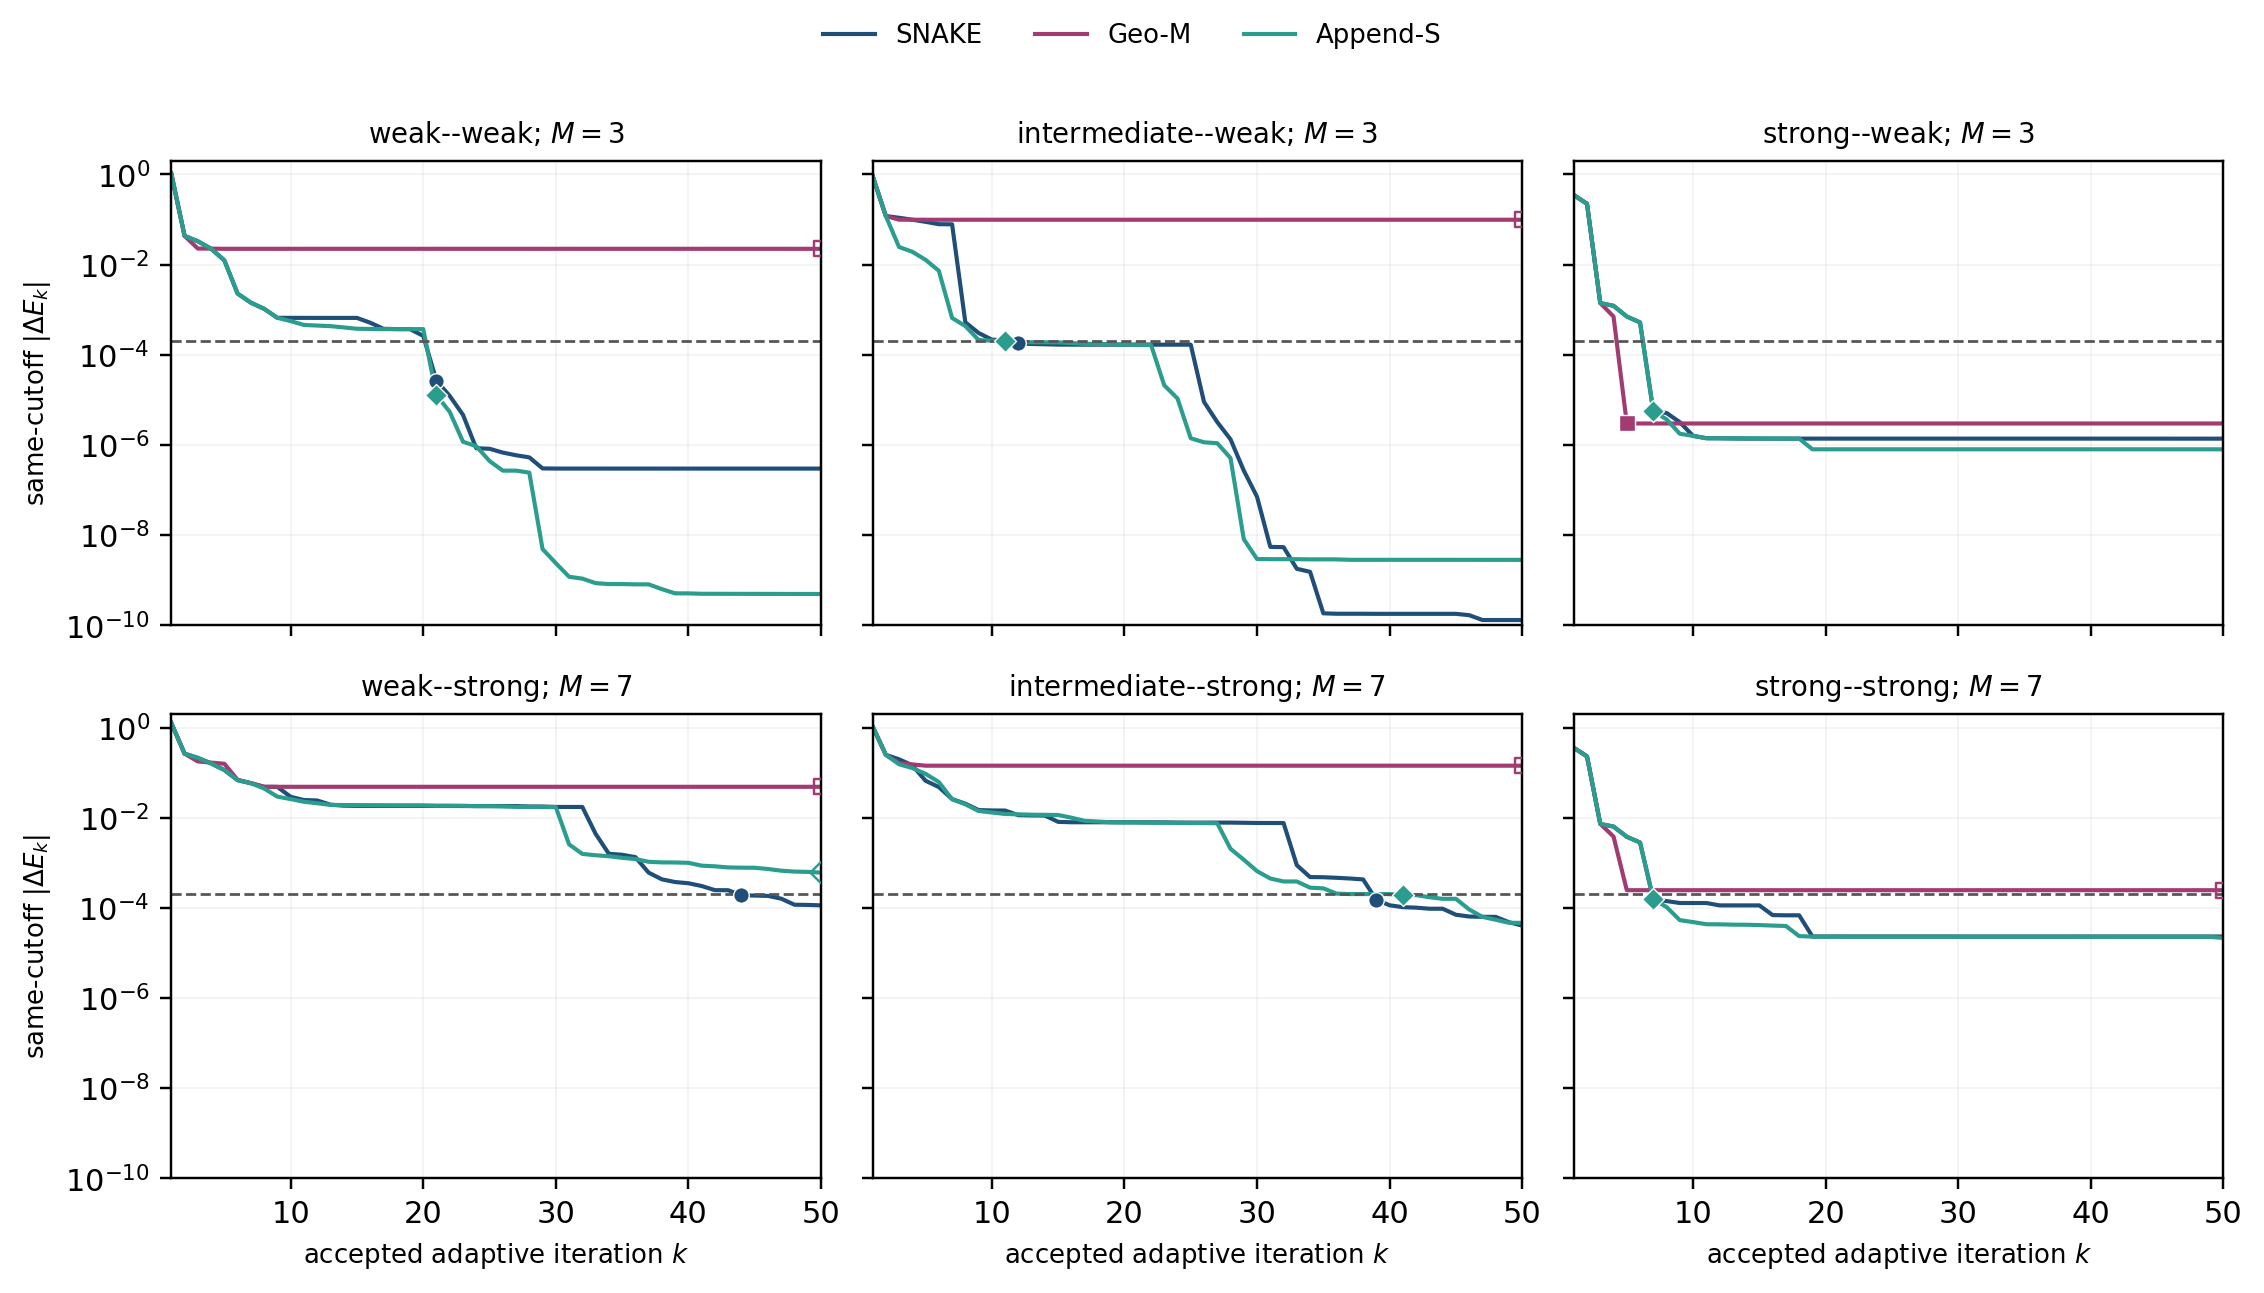
\includegraphics[width=0.98\textwidth]{figures/paper_i_hh_first_hit_20260721/paper_i_hh_first_hit_trajectories_20260721.pdf}
\captionof{figure}{Same-cutoff Hubbard--Holstein energy-error trajectories through 50 accepted adaptive iterations. The dashed line marks the fixed reporting target $E_T=2\times10^{-4}$. Filled symbols mark the first target crossing; open symbols at $k=50$ identify methods that do not reach the target. The top row uses $M=3$ for weak-Holstein sectors and the bottom row uses $M=7$ for strong-Holstein sectors. SNAKE is the support-projected, non-whitened Phase-III route with source-metric no-overlap trust calibration and supported-Fubini--Study-whitened accepted refits. Geo-M and Append-M use intact macro generators; Append-S uses symmetry-guarded projected-singleton children.}
\label{fig:hh_main_results_composite}
\end{center}
\end{minipage}
\clearpage
\noindent\begin{minipage}{\textwidth}
\begin{center}
\captionof{table}{Fixed-accuracy Hubbard--Holstein comparison at the first accepted prefix satisfying 
\(\lvert\Delta E_k\rvert\le 2\times10^{-4}\). ``NR'' means that the method did not reach the target by $k=50$; the error shown for an NR row is its best observed error, and resource cells are intentionally blank. Qiskit costs use \texttt{table\_i\_basis\_gate\_transpile\_v1}; $S_{\rm alg}$ is the closed cumulative logical estimator ledger through the same prefix. Macro and projected-singleton rows expose different candidate representations and are labeled separately.}
\label{tab:hh_fixed_accuracy_first_hit}
\scriptsize
\setlength{\tabcolsep}{3.0pt}
\renewcommand{\arraystretch}{0.94}
\begin{tabular}{@{}llrrrrrr@{}}
\toprule
Regime & Method (pool) & $k_{\rm eval}$ & \(\lvert\Delta E\rvert\) & $N_{2q}$ & $D_{2q}$ & $D_c$ & $S_{\rm alg}$ \\
\midrule
weak--weak & SNAKE & 21 & 2.6510e-05 & 74 & 60 & 314 & 19,381 \\
 & Geo-M & NR & best 2.2452e-02 & -- & -- & -- & -- \\
 & Append-M & NR & best 4.8937e-04 & -- & -- & -- & -- \\
 & Append-S & 21 & 1.2606e-05 & 90 & 70 & 371 & 70,320 \\
\addlinespace[1.5pt]
intermediate--weak & SNAKE & 12 & 1.7874e-04 & 40 & 32 & 191 & 6,226 \\
 & Geo-M & NR & best 9.9076e-02 & -- & -- & -- & -- \\
 & Append-M & NR & best 2.6707e-02 & -- & -- & -- & -- \\
 & Append-S & 11 & 1.9893e-04 & 46 & 34 & 178 & 23,329 \\
\addlinespace[1.5pt]
strong--weak & SNAKE & 7 & 5.6271e-06 & 18 & 11 & 96 & 2,366 \\
 & Geo-M & 5 & 2.9972e-06 & 144 & 116 & 723 & 39,701 \\
 & Append-M & 5 & 2.9972e-06 & 144 & 116 & 723 & 1,579 \\
 & Append-S & 7 & 5.6271e-06 & 18 & 12 & 97 & 13,511 \\
\midrule
weak--strong & SNAKE & 44 & 1.9034e-04 & 148 & 97 & 595 & 203,325 \\
 & Geo-M & NR & best 4.8528e-02 & -- & -- & -- & -- \\
 & Append-M & NR & best 3.9617e-02 & -- & -- & -- & -- \\
 & Append-S & NR & best 6.0595e-04 & -- & -- & -- & -- \\
\addlinespace[1.5pt]
intermediate--strong & SNAKE & 39 & 1.5008e-04 & 128 & 68 & 485 & 145,669 \\
 & Geo-M & NR & best 1.4271e-01 & -- & -- & -- & -- \\
 & Append-M & NR & best 2.4495e-02 & -- & -- & -- & -- \\
 & Append-S & 41 & 1.9221e-04 & 238 & 186 & 739 & 829,124 \\
\addlinespace[1.5pt]
strong--strong & SNAKE & 7 & 1.5515e-04 & 18 & 11 & 96 & 2,799 \\
 & Geo-M & NR & best 2.4689e-04 & -- & -- & -- & -- \\
 & Append-M & 9 & 1.3924e-04 & 904 & 681 & 3,757 & 5,713 \\
 & Append-S & 7 & 1.5515e-04 & 18 & 12 & 107 & 63,838 \\
\bottomrule
\end{tabular}
\end{center}
\end{minipage}
\clearpage
\twocolumngrid
\par\addvspace{0.45ex}
SNAKE reaches the fixed target in all six regimes. Geo-M reaches it only in
strong--weak, Append-M reaches it in strong--weak and strong--strong, and
Append-S reaches it in five regimes, missing only weak--strong by $k=50$.
Over the five regimes in which both SNAKE and Append-S reach the target, the
summed SNAKE resources are $278/182/1{,}182$ for
$N_{2q}/D_{2q}/D_c$ and $176{,}441$ for $S_{\rm alg}$, compared with
$410/314/1{,}492$ and $1{,}000{,}122$ for Append-S. These correspond to
reductions of $32\%$, $42\%$, $21\%$, and $82\%$, respectively.
The macro and singleton rows are retained together to expose pool sensitivity;
they are not treated as a pool-matched comparison.
\par\addvspace{1.0ex}
% BEGIN_DRAFT_HH_CHILD_FAIRNESS_PROSE_TODO_20260624
% Condensed future-prose note; comment only, do not render yet.
% Use the native-forced SPSA Pauli-child protocol as the main displayed HH comparison.
% Treat monotone/non-forced rows as sensitivity evidence: Append and Geo improve under monotone,
% while SNAKE is stronger in the native-forced child+Schur condition or comparable to monotone.
% No-child SNAKE hurts under the current parameterization; phrase this as a hyperparameter/
% Optuna/settings limitation, not as an intrinsic limitation of SNAKE.
% Schur warm-start versus no-Schur warm-start did not materially change same-cutoff
% energy error in this comparison; treat Schur as a refit/conditioning and cost-shaping
% mechanism unless a later source-locked replay shows an accuracy separation.
% Candidate claim: native-forced SNAKE child+Schur versus Geo monotone no-child gives
% same-order aggregate same-cutoff energy accuracy with much smaller SNAKE compiled circuit cost.
% Shot/work costs remain pending under a common accounting convention.
% Avoid overclaiming: strong--weak is the visible outlier in the compact comparison.
% Source support: output/pdf/paper_i_hh_child_fairness_20260623/
% paper_i_hh_child_fairness_compact_child_schur_20260623.{pdf,json,csv}.
% END_DRAFT_HH_CHILD_FAIRNESS_PROSE_TODO_20260624
\par\addvspace{1.0ex}

% BEGIN_MACHINE_READABLE_WEAK_WEAK_SNAKE_MECHANISM_ABLATION_TERMINAL_METRICS_20260709
% {"schema":"paper_i_weak_weak_snake_mechanism_ablation_terminal_delta_metrics_v4","updated_date":"2026-07-09","table_labels":["tab:weak_weak_snake_mechanism_ablation_terminal_metrics"],"support_pdf":"output/pdf/paper_i_hh_weak_weak_snake_mechanism_ablation_20260708/paper_i_hh_weak_weak_snake_mechanism_ablation_20260708.pdf","support_json":"output/pdf/paper_i_hh_weak_weak_snake_mechanism_ablation_20260708/paper_i_hh_weak_weak_snake_mechanism_ablation_20260708.json","support_json_sha256":"07304f5bec8b71f8bf3ce29b2f1613899d74937e889af78cfcdfaf859f1630f6","source_table_page":"support PDF page 7, terminal-iteration metrics promoted as delta-from-anchor table","row_policy":"source-anchor row omitted because all deltas are zero; no-shortlisting omitted; Status column omitted; batch-cap rows omitted pending corrected batching audit because audited batch-cap trajectories did not admit multi-record batches","benchmark":"weak--weak Hubbard--Holstein","optimizer":"POWELL","terminal_depth_contract":"terminal iteration-prefix deltas at k=30 relative to Source anchor; k column omitted from rendered table","rounding_policy":"Delta energy-error percent rounded to integer except no-batching, no-prune, and no-cost-term rows keep one decimal place"}
% END_MACHINE_READABLE_WEAK_WEAK_SNAKE_MECHANISM_ABLATION_TERMINAL_METRICS_20260709
\noindent\begin{minipage}{\columnwidth}
\captionof{table}{\label{tab:weak_weak_snake_mechanism_ablation_terminal_metrics}Weak--weak Hubbard--Holstein SNAKE mechanism ablations at the terminal 30-iteration prefix. Entries are differences from the source anchor in the terminal-iteration support table; the source-anchor row is omitted because all deltas are zero. Here \(d\) is the number of generators in the terminal ansatz. The energy-error column is a percent change, while circuit-resource and estimator-work columns are absolute integer deltas. \(\Delta S\) is computed from terminal branch-local \(S_{\rm alg}\). Batch-cap rows are omitted pending a corrected batching audit.}
\centering
\scriptsize
\setlength{\tabcolsep}{1.2pt}
\renewcommand{\arraystretch}{1.02}
\resizebox{\columnwidth}{!}{%
\begin{tabular}{@{}lrrrrrr@{}}
\toprule
Variant & $\Delta|\Delta E|$ (\%) & $\Delta d$ & $\Delta N_{\twq}$ & $\Delta D_{\twq}$ & $\Delta D_c$ & $\Delta S$ \\
\midrule
No batching reference & 1.0 & 0 & -2 & -12 & -67 & -271 \\
No prune & 1.3 & 10 & 34 & 23 & 116 & 706 \\
No cost term & 1.4 & -2 & -6 & -12 & -52 & 574 \\
No Phase III & 202 & -10 & 114 & 59 & 550 & 40823 \\
Phase I only; macro pool & 202 & -12 & 182 & 117 & 883 & 26538 \\
Phase I only; singleton pool & 202 & -5 & 24 & 15 & 229 & 19949 \\
Full-ansatz geometry & 8 & -1 & -10 & -16 & -88 & -530 \\
\bottomrule
\end{tabular}%
}
\end{minipage}
\par\addvspace{1.0ex}

\section{Discussion and conclusion}
\label{sec:discussion}
\label{sec:conclusion}

% Struct label: Mechanistic interpretation
SNAKE's second-order model combines the Fubini--Study metric with joint candidate and active-ansatz response to estimate the energy reduction available after ansatz relaxation. These estimates are weighted by generator-specific circuit and estimator costs during candidate ranking. The primary empirical comparison evaluates those resources at a shared energy-error target, so resource differences are measured at matched accuracy. SNAKE reaches this target in all six Hubbard--Holstein regimes. The intact-macro Geo-ADAPT and Append-ADAPT comparators reach it in one and two regimes, respectively, while projected-singleton Append-ADAPT reaches it in five. Across those five common target hits, SNAKE reduces the summed two-qubit count, two-qubit depth, total circuit depth, and logical estimator work by $32\%$, $42\%$, $21\%$, and $82\%$, respectively.

In the displayed Hubbard--Holstein evidence route, shortlisting, singleton response modeling, a supported Fubini--Study Phase-III solve, and adaptive trust control remain active, while batching, beam continuation, and generator ablation are disabled. The latter mechanisms remain optional SNAKE extensions and require separate ablation evidence; they are not invoked to explain the selected errors reported here.

% Struct label: Scope and limitations
Despite targeting NISQ-era constraints, the present results are noiseless and use small, classically solvable two-site models. Further work should compare noise models and noise-aware stopping criteria for ADAPT algorithms. Finite-shot confidence envelopes, backend-resolution floors, and iteration-dependent gate-selection breadth and mechanistic pressures remain prospective SNAKE extensions. Further work may focus on lane partitioning in shortlists and pruning behavior based on the physical process the operator encodes, such as UCCSD vs a polaronic operator.
% Struct label: Summary/so what
Variational quantum eigensolvers remain an important approach for simulating physical systems on near-term quantum hardware. SNAKE extends ADAPT-VQE by explicitly incorporating state geometry, measurement burden, and hardware constraints into generator selection. Its principal empirical test is the circuit and estimator cost required to reach the same energy-error target as the adaptive comparators, including for mixed fermion--boson systems. The Hubbard--Holstein operator pool is defined by the physical lanes in Appendix~\ref{app:lane_shortlisting}, with the spin-boson/Rabi pool defined in Appendix~\ref{app:spin_boson_rabi}.

\appendix
\section{THIS MIGHT BELONG HERE OR ELSEWHERE -- Saved work for possible coherent-implementation}

We now explain a method to partition the record set based on an operators physical response type; This enables more aggressive shortlisting with less risk of omitting a unique response channel. See App.~(\ref{subsec:hh_physical_operator_lanes}) for the six defined lanes. However, a lane can still be retired if it's highest-scored record is lower than a parametrized fraction of the highest-scored record in the global lane-agnostic record set.

We denote the partition of \(\mathcal R\) by partitioning \(\mathcal G\). Let \(\mathcal L\) be the fixed set of
physical lane labels, and let \(\lambda:\mathcal G\to\mathcal L\) map each
generator to its physical operator-type label. For \(r=(A,p)\), write
\(\lambda(r):=\lambda(A)\).

For each lane represented in \(\mathcal R^{(t)}\), define the lane-wise inherited
record set by
\begin{equation*}
\mathcal R_{\ell}^{(t)}
=
\left\{
r\in\mathcal R^{(t)}
:
\lambda(r)=\ell
\right\}.
% source label: eq:lane_phase_records
\end{equation*}
For each retained lane, let its representative record be the within-lane
maximizer
\[
r_{\ell}^{\star}
\in
\operatorname*{arg\,max}_{r\in\mathcal R_{\ell}^{(t)}}
S^{(t)}(r).
\]
Let \(\mathcal L^{(t)}\subseteq\mathcal L\) denote the lane labels that remain
live at phase \(t\). A represented lane \(\ell\) remains live when
\begin{equation}
\ell\in\mathcal L^{(t)}
\quad\Longleftrightarrow\quad
S^{(t)}(r_{\ell}^{\star})
\ge
\tau_t
\max_{r\in\mathcal R^{(t)}}S^{(t)}(r).
\label{eq:phase_restriction_map}
\end{equation}
Here \(\tau_t\in[0,1]\) is the phase-\(t\) relative lane-retention threshold.
The number of live lanes that receive protected representatives is
\begin{equation}
\min\left\{
N_t,\,
\left\lceil \eta_t|\mathcal L^{(t)}|\right\rceil
\right\},
\qquad
|\mathcal R^{(t)}|\le N_t ,
\label{eq:phase_lane_budget}
\end{equation}
where \(N_t\) is the phase-\(t\) global retained-record cap and
\(\eta_t\in[0,1] \) is the live-lane protection fraction. A retained lane has at least it's highest scored record. The remaining record set is scored scored globally and the top-scored records are then allocated to their respective lane.

For the present procedure, the lane rule is invoked at \(t=1\), so
\(\mathcal R^{(2)}:=\mathcal R^{(1)}\). Phase II evaluates
Eq.~\eqref{eq:phase2_gain} and keeps the highest-scoring records under its
fixed effective cap \(N_2\):
\begin{equation*}
\mathcal R^{(2)}
=\operatorname{Top}_{\min\{N_2,|\mathcal R^{(2)}|\}}
\left(\mathcal R^{(2)};S^{(2)}\right).
\end{equation*}
Pauli splitting and symmetry applied to \(\mathcal R^{(2)}\) give
\(\mathcal R^{(3)}\). The six
Hubbard--Holstein physical lane labels are defined in
Appendix~\ref{app:lane_shortlisting}. All candidate derivatives, geometric
blocks, and resource estimates are evaluated relative to the same optimized
state \(\ket{\psi_k}\); the enlarged ansatz is refitted after Phase III
returns a proposal. The phase gains and cost-weighted score are defined in
Sec.~\ref{subsec:candidate_energy_models}.

\section{Physical-response lane shortlisting}
\label{app:lane_shortlisting}

\subsection{Hubbard--Holstein physical operator lanes}
\label{subsec:hh_physical_operator_lanes}
%
\noindent
To prevent a numerically gradient-dominant cluster of similar physical-response-type records from dominating the record set advanced to the next phase, we partition the inherited record set by physical response channel. 

Between Phases I and II, \textsc{SNAKE} partitions Hubbard--Holstein
generator--position records into six lanes according to the physical response
encoded by the generator \(A\). Applying the retention rule
within this partition prevents clusters of physically similar records from
exhausting the global shortlist while leaving the phase score \(S^{(t)}\)
unchanged. Competitive representatives of electronic correlation, electronic
transport, phonon displacement, phonon relaxation, electron--phonon dressing,
and Hamiltonian-block motion therefore remain exposed before directional
curvature and full-response measurements are incurred.

\paragraph*{Electronic UCCSD lane.}
This lane contains bare electronic single- and double-excitation generators,
tensored with the phonon identity:
\begin{align*}
G_{i\to a,\sigma}
&=
\ii(c_{a\sigma}^{\dagger}c_{i\sigma}
-c_{i\sigma}^{\dagger}c_{a\sigma}),\\
G_{ij\to ab,\sigma\sigma'}
&=
\ii(c_{a\sigma}^{\dagger}c_{b\sigma'}^{\dagger}
c_{j\sigma'}c_{i\sigma}
-{\rm h.c.}) .
\end{align*}
Here \(i,j\) label occupied spin orbitals, \(a,b\) label virtual spin orbitals,
\(\sigma,\sigma'\in\{\uparrow,\downarrow\}\), and \(c^\dagger,c\) are
fermionic creation and annihilation operators. This lane targets electronic
correlation without explicit phonon dressing.

\paragraph*{Electronic hopping/current lane.}
This lane contains purely electronic Hubbard transport, density-assisted
transport, pair-hop/current, and exchange/current channels, all acting with the
phonon identity. The spin-summed hopping and current generators are
\begin{align*}
T_{ij}
&=
\sum_{\sigma}
(c_{i\sigma}^{\dagger}c_{j\sigma}
+c_{j\sigma}^{\dagger}c_{i\sigma}),\\
J_{ij}
&=
\ii\sum_{\sigma}
(c_{i\sigma}^{\dagger}c_{j\sigma}
-c_{j\sigma}^{\dagger}c_{i\sigma}) .
\end{align*}
Density-assisted channels multiply \(T_{ij}\) or \(J_{ij}\) by local fermion
number operators. Pair-hop/current channels move an onsite spin pair between
sites. Exchange/current channels exchange spin-resolved occupations across a
bond. This lane targets lattice electronic motion beyond bare UCCSD excitation
structure.

\paragraph*{Phonon-cloud lane.}
This lane contains pure phonon displacement, momentum, and occupation channels.
Here \(b_i^\dagger,b_i\) are phonon creation and annihilation
operators on site or mode \(i\), and
\[
X_i=b_i+b_i^\dagger,
\qquad
P_i=\ii(b_i^\dagger-b_i),
\qquad
n_{b,i}=b_i^\dagger b_i .
\]
The Hubbard--Holstein lane includes the local phonon generators \(X_i\),
\(P_i\), and \(n_{b,i}\), together with nonlocal charge--phonon cloud terms
listed below in the dressed electron--phonon lane. This lane targets the
displacement and occupation response of the phonon cloud before explicit
electronic conditioning is applied.

\paragraph*{Phonon-relaxation lane.}
This lane contains pure phonon squeeze, width, quadratic, and nonlinear
channels:
\begin{align*}
S_i&=\ii[(b_i^\dagger)^2-b_i^2],\\
&X_i^2,\quad P_i^2,\quad n_{b,i}^2,\quad
X_iP_i+P_iX_i .
\end{align*}
This lane targets changes in local phonon width, occupation curvature, and
cutoff-sensitive nonlinear response.

\paragraph*{Dressed electron--phonon lane.}
This lane contains generators that explicitly couple electronic charge or bond
motion to phonon response. With
\[
D_i=n_i-\bar n I,
\qquad
Q_i=n_{i\uparrow}n_{i\downarrow},
\]
it includes local polaronic channels \(D_iP_i\) and \(D_iS_i\), nonlocal
charge--phonon channels \(D_iP_j\) and \(D_iX_j\), doublon-conditioned channels
\(Q_iP_j\) and \(Q_iX_j\), and bond-dressing channels
\begin{align*}
&T_{ij}(P_i-P_j),
\qquad
J_{ij}(P_i-P_j),\\
&T_{ij}(P_i+P_j),
\qquad
T_{ij}(P_i-P_j)^2,\\
&J_{ij}(P_i-P_j)^3 .
\end{align*}
It also includes UCCSD electronic generators multiplied by phonon-dressing
operators, including product and sequential electronic/phonon motif generators.
This lane targets polaron formation, density-conditioned lattice response,
doublon-conditioned lattice response, and bond-conditioned electron--phonon
dressing.

\paragraph*{Hamiltonian-block lane.}
This lane contains grouped physical blocks of the Hubbard--Holstein Hamiltonian
in Eq.~\eqref{eq:hubbard_holstein_static}: electronic hopping, onsite
interaction, phonon energy, and electron--phonon coupling blocks, together with
the full Hamiltonian-block rotation when included. It also includes
Hamiltonian-term generators and their quadrature partners. This lane preserves
coarse Hamiltonian structure as candidate ansatz motion.

Here the Phase-I records are ordered by \(S^{(1)}\) and retained under
Eqs.~\eqref{eq:phase_restriction_map}--\eqref{eq:phase_lane_budget}. The lane
map changes shortlist allocation only; it does not modify the score assigned to
any record. The resulting retained set is the input to Phase II.


\section{Numerical conventions}
\label{app:numerical_conventions}

\paragraph*{Scalar phase solves.}
When \(H_{rr}>0\), the maximizing Phase-II candidate amplitude is
\begin{equation}
\alpha_2^\star(r)
=-\operatorname{sgn}[g(r)]
\min\!\left\{
\frac{|g(r)|}{H_{rr}},
\frac{\rho_k}{\sqrt{G_{rr}}}
\right\}.
\label{eq:phase2_alpha_star}
\end{equation}
When \(H_{rr}\le0\), the Phase-II maximizer lies on the trust boundary unless
both \(g(r)\) and \(H_{rr}\) vanish. For \(g(r)\ne0\), its sign is opposite to
\(g(r)\). If \(g(r)=0\) and \(H_{rr}<0\), the two boundary points are
degenerate maximizers; when \(g(r)=H_{rr}=0\), the maximizing amplitude is
taken to be zero. Phase I has the boundary maximizer
\(\alpha_1^\star(r)=-\operatorname{sgn}[g(r)]\rho_k/\sqrt{G_{rr}}\).

\paragraph*{Phase-III trust boundary.}
The trust-boundary multiplier \(\lambda\ge0\), distinct from the stabilization
included in \(\widetilde{\mathbf R}\), satisfies
\begin{equation}
\begin{aligned}
(\widetilde{\mathbf R}+\lambda\widetilde{\mathbf G})
\widetilde{\mathbf z}^{\star}
&=-\widetilde{\mathbf b},\\
\lambda\left[
\rho_k^2-(\widetilde{\mathbf z}^{\star})^{\top}
\widetilde{\mathbf G}\widetilde{\mathbf z}^{\star}
\right]&=0.
\end{aligned}
\label{eq:phase3_joint_kkt}
\end{equation}
Thus \(\lambda=0\) for an interior solution, while a binding trust boundary
determines a positive multiplier.

\paragraph*{Radius-update safeguards.}
In Eq.~\eqref{eq:adaptive_trust_radius}, \(\varepsilon_\rho>0\) prevents
division by zero. A contracting proposal is applied directly. An expanding
proposal is accepted only when the Phase-III solution reached the trust
boundary and the complete refit decreased the energy; a vetoed expansion
leaves \(\rho_{k+1}=\rho_k\).


\section{Optional batch admission}
\label{app:batching}

To admit several favorable records without introducing redundant tangent
directions, \textsc{SNAKE} evaluates compatible Phase-III records jointly under
the batch trust-region model.

Let \(b_{\max}\) be the configured batch-size cap, and let
\(\mathfrak B_k\subseteq
2^{\mathcal R^{(3)}}\setminus\{\varnothing\}\) contain exactly the
batches \(B\) with \(|B|\le b_{\max}\) for which every distinct pair
\(r,r'\in B\) has disjoint generator support and satisfies
\([A_r,A_{r'}]=0\). Here \(A_r\) is the generator carried by record \(r\).
Let
\(B=\{r_1,\ldots,r_s\}\in\mathfrak B_k\).

Let
\(\boldsymbol\alpha_B=(\alpha_1,\ldots,\alpha_s)^{\top}\) and
\(\mathbf g_B=(g(r_1),\ldots,g(r_s))^{\top}\). Replacing the scalar candidate
coordinate in Eq.~\eqref{eq:local_quadratic} by \(\boldsymbol\alpha_B\) gives
\begin{equation*}
\begin{aligned}
\mathbf z&=
\begin{pmatrix}
\boldsymbol\alpha_B\\
\delta\boldsymbol\theta
\end{pmatrix},
&
\mathbf b&=
\begin{pmatrix}
\mathbf g_B\\
\mathbf 0
\end{pmatrix}.
\end{aligned}
\end{equation*}
The Hessian and Gram matrices are assembled from
Eq.~\eqref{eq:joint_response_entries} over these \(s\) candidate coordinates
and all active coordinates. Applying the supported construction and joint
solve of Eqs.~\eqref{eq:phase3_supported_blocks}--\eqref{eq:phase3_joint_gain}
yields \(\Delta E_3(B)\) and the lifted optimizer
\(\mathbf z_3^\star(B)=V\widetilde{\mathbf z}^{\star}\). Its predicted
Fubini--Study displacement is
\begin{equation*}
d_3(B)
=\sqrt{(\mathbf z_3^\star(B))^{\top}
\mathbf G\mathbf z_3^\star(B)}.
\end{equation*}
The quantity \(K_3(B)\) is the cost term from
Eq.~\eqref{eq:hardware_cost_sum} evaluated over the batch. The admitted batch
is therefore
\begin{equation}
B_k^\star\in\arg\max_{B\in\mathfrak B_k}
\frac{\Delta E_3(B)}{K_3(B)}.
\label{eq:batch_argmax}
\end{equation}
Equation~\eqref{eq:batch_argmax} is the combinatorial search ideal, with a
score-ordered greedy admission serving as a measurement-cheap practical
approximation.

\section{Optional beam continuation and generator ablation}
\label{app:optional_structure_management}

\subsection{Beam continuation}
A generator that is favorable for the current ansatz can become unfavorable
after later insertions alter its commutation context and the circuit is
refitted; committing to that generator can also preclude a generator that
remains favorable along a different growth path. \textsc{SNAKE} may therefore use
Lowerre-style beam search \cite{Lowerre1976Beam} to refit multiple competitive
child branches within a fixed-width beam. Given a score-ordered top-$N$
proposal list, whose entries may be singleton records or optional batches from
Appendix~\ref{app:batching}, a parent branch can spawn $N$ children, each
differing by the proposal admitted to it. The cost of this parallel beam
universe is increased total hardware-graph and qubit support across child
branches. When ablation is enabled, each child branch then undergoes the
generator-ablation procedure described next. After refit and ablation, let
\(E_{\rm root}\) be the common beam-root energy, \(E_b\) the realized branch
energy, and \(\Delta K_b\) the cumulative added branch burden. Branches that are
strictly Pareto dominated in \((E_b,\Delta K_b)\) are removed. The remaining
branches are ordered by realized energy gain per added cost,
\begin{equation*}
\Phi_b=\frac{E_{\rm root}-E_b}{1+\Delta K_b},
\end{equation*}
Let \(B_{\rm live}\ge1\) denote the configured beam width. The top
\(B_{\rm live}\) branches are retained, and the leading retained branch is
the current output branch.


\subsection{Generator ablation}
%
When generator ablation is enabled after an admission and inner refit,
\textsc{SNAKE} tests whether an active
generator can be removed while its state displacement and energy contribution
are recovered by the surviving coordinates. A metric-regularized Schur
deletion surrogate returns the compensating shift
\(\delta\boldsymbol\theta^\star\) and predicted deletion loss
\(\Lambda(d)\) for an ablation record \(d\); candidates are nominated by predicted loss per relieved
resource cost and retained only after an explicit delete--refit energy check.

Let \(\mathbf A_k=(A_1,\ldots,A_{n_k})\) be the ordered generator sequence
defining the current optimized ansatz \(U_k(\boldsymbol\theta_k^\star)\).
Each active generator \(A_j\) carries an admission step \(a_j\) and a cooldown
counter \(c_j(k)\). Equivalently, if \(\hat r_j\) is the most recent rejected
delete/refit trial for \(A_j\), a fixed cooldown requires
\(k-\hat r_j\ge\tilde c\); if no such rejection exists, the cooldown condition
is satisfied. An ablation record \(d=(A,p)\) separates an active generator
\(A\) from its current ansatz position \(p\). The eligible record set is
\begin{equation*}
\mathcal D_k
=
\left\{
d=(A_j,j)
:
k-a_j\ge \tilde p,\;
c_j(k)\le0
\right\}.
% source label: eq:eligibility_set
\end{equation*}
Here \(\tilde p\) and \(\tilde c\) are run-time constant protection thresholds.

For \(d=(A,p)\in\mathcal D_k\), let \(\beta\) be the displacement along the
record coordinate. Complete deletion is evaluated at
\(\beta=-\theta_{k,p}^\star\), while
\(\delta\boldsymbol\theta\in\mathbb R^{n_k-1}\) is the response of the
remaining ansatz coordinates. The position-resolved derivative \(g(d)\), the
energy Hessian \(H\), and the Fubini--Study Gram matrix \(G\) follow the same
definitions as in Phases I--III and are evaluated at
\(U_k(\boldsymbol\theta_k^\star)\). The linear term in
\(\delta\boldsymbol\theta\) vanishes at the refitted optimum; residual
survivor-coordinate gradients from incomplete inner optimization are
neglected.

Before forming the ablation blocks, the measured Hessian and metric are
projected onto their positive-semidefinite parts, which we continue to denote
by \(H\) and \(G\). Define the metric-regularized quadratic form
\[
\mathcal Q:=H+\eta G,
\]
where \(\eta\ge0\) controls the Fubini--Study regularization. The deletion
specialization of the Phase-III block surrogate is
\begin{equation}
\Lambda(d)
=
\min_{\delta\boldsymbol\theta}
\left[
g(d)\beta
+\frac12
\begin{pmatrix}
\beta\\
\delta\boldsymbol\theta
\end{pmatrix}^{\!\top}
\begin{pmatrix}
\mathcal Q_{dd} & \mathcal Q_{d\theta}\\
\mathcal Q_{\theta d} & \mathcal Q_{\theta\theta}
\end{pmatrix}
\begin{pmatrix}
\beta\\
\delta\boldsymbol\theta
\end{pmatrix}
\right].
\label{eq:schur_metric_prune}
\end{equation}
The optimal Schur response becomes
\begin{equation*}
\delta\boldsymbol\theta^\star
=
-\beta\mathcal Q_{\theta\theta}^{-1}\mathcal Q_{\theta d}.
% source label: eq:ablation_schur_response
\end{equation*}
Substitution into Eq.~\eqref{eq:schur_metric_prune} gives
\begin{equation*}
\Lambda(d)
=
\left[
g(d)\beta
+\frac{\beta^2}{2}
\left(
\mathcal Q_{dd}
-\mathcal Q_{d\theta}
\mathcal Q_{\theta\theta}^{-1}
\mathcal Q_{\theta d}
\right)
\right].
% source label: eq:ablation_schur_loss
\end{equation*}

To prefer deletions that relieve larger compiled and measurement burden, let
\(K(d)\) be the same normalized hardware/shot-cost denominator used in the SNAKE
candidate scores, evaluated over the current ansatz-entry population. The
metric-regularized Schur surrogate nominates generators whose predicted
deletion loss is small relative to the hardware and estimator burden they
remove. The ratio
\(\Lambda(d)/K(d)\) is clipped to the interval \([0,1]\) before nomination.
The nominated ablation record is determined by
\begin{equation*}
d^\star
\in
\operatorname*{arg\,min}_{d\in\mathcal D_k}
\frac{\Lambda(d)}{K(d)},
\qquad
\frac{\Lambda(d^\star)}{K(d^\star)}
\le
\epsilon .
% source label: eq:ablation_nomination
\end{equation*}
If the second condition fails, no ablation is nominated at this adaptive step.
After a candidate deletion, the ablation is accepted only if the realized energy
loss \(\Delta E(d^\star)\) is no larger than the smaller of the absolute
ablation tolerance \(\epsilon\) and the fractional recent-gain tolerance
\(\zeta\left(E(U_{k-1})-E(U_k)\right)\), where \(0\le\zeta\le1\).

If this acceptance gate rejects the trial ablation, the post-refit
branch remains \(U_k(\boldsymbol\theta_k^\star)\). The same Gram and Hessian
blocks are then reused in Eqs.~\eqref{eq:phase3_joint_gain}
and~\eqref{eq:phase3_geometry}.
The Phase-III displacement coordinates are local
shifts, \(\boldsymbol\theta=\boldsymbol\theta^\star+
\delta\boldsymbol\theta\), so derivatives at
\(\delta\boldsymbol\theta=\mathbf 0\) reuse the same
\(G_{\theta\theta}\) and \(H_{\theta\theta}\) blocks. Conversely, if the acceptance gate accepts the ablation, subsequent Phase-II/III
scoring recomputes the Gram and Hessian blocks on the refit pruned circuit
for \(d^\star=(A^\star,p^\star)\):
\(U_k^{\ominus}((\boldsymbol\theta_k^\star)_{\setminus p^\star})
=
U_k(\boldsymbol\theta_k^\star)\ominus
\exp(-i\theta_{k,p^\star}^\star A^\star)\), where \((\boldsymbol\theta_k^\star)_{\setminus p^\star}\) represents the optimized circuit parameterization after removing position \(p^\star\).




\section{Total estimator-query accounting}
\label{app:estimator_queries}
The \(S\) column gives the logical scalar estimator-query count accumulated
through the fixed-accuracy reporting prefix in
Eq.~\eqref{eq:fixed_accuracy_prefix}. One query is one scalar expectation-value
primitive used by the algorithm at the relevant prepared state, such as a
candidate-gradient scalar, a Fubini--Study norm scalar, a Gram/metric entry, a
curvature/Hessian/coupling entry, or one Hamiltonian objective evaluation in an
optimizer/refit. Algebraic recombination, ranking, pseudoinverse solves, Schur
complements, and other classical postprocessing are not additional queries.
Same-state reuse and symmetry are applied: a scalar primitive reused by
multiple formulas at the same prepared state is counted once, and symmetric
matrix entries are counted once. The same primitive evaluated at a different
accepted-prefix state or optimizer/refit trial state counts again. Thus \(S\)
is not a physical-shot count, raw Pauli-word count, or post-Pauli-grouped
measurement-setting count.

Let \(k\) index accepted adaptive iterations, and let \(k_{\rm eval}\) be
the method- and regime-specific prefix in Eq.~\eqref{eq:fixed_accuracy_prefix}.
For append-only ADAPT, let \(\mathcal A_k\) be the live candidate set scored
before the \(k\)-th admission, with \(n_k=|\mathcal A_k|\). The
candidate-gradient scan contributes \(n_k\). For Geo-ADAPT, the tangents
\(\tau_r^{(k)}=(I-|\psi_k\rangle\langle\psi_k|)(-iA_r|\psi_k\rangle)\)
define \(G_{rs}^{(k)}=\Re\langle\tau_r^{(k)},\tau_s^{(k)}\rangle\) for
\(r,s\in\mathcal A_k\), adding \(n_k(n_k+1)/2\) symmetric metric-entry
queries. If \(f_k\) is the number of Hamiltonian objective evaluations used
by the refit optimizer after the \(k\)-th admission, then
\begin{equation*}
\begin{aligned}
S_{\rm ADAPT}
&=
\sum_{k=0}^{k_{\rm eval}}
\left(n_k+f_k\right),
\\
S_{\rm Geo}
&=
\sum_{k=0}^{k_{\rm eval}}
\left(n_k+\frac{n_k(n_k+1)}{2}+f_k\right).
\end{aligned}
% source label: eq:appendix_s_adapt_geo
\end{equation*}

For SNAKE, let \(P_\ell(k)\), with \(\ell=1,2,3\), denote the scalar-primitive sets requested or made available by Phase \(\ell\) before the \(k\)-th admission, before de-duplication against earlier phases. If \(f_k\) is the number of Hamiltonian objective evaluations used by the optimizer and refit checks after the \(k\)-th admission, then
\begin{align}
S_{\rm SNAKE}
&=
\sum_{k=0}^{k_{\rm eval}}
\left[
|P_1(k)|+|P_2(k)\setminus P_1(k)|
\right.
\nonumber\\
&\qquad\left.
 +|P_3(k)\setminus(P_1(k)\cup P_2(k))|
+f_k
\right].
\label{eq:appendix_s_snake}
\end{align}

The set subtractions in Eq.~\eqref{eq:appendix_s_snake} implement same-prefix reuse across phases. Pauli decompositions, compatible-Pauli grouping, shot allocation, and grouped measurement settings are lower-level measurement diagnostics and are not resolved in the reported \(S\) column; they enter only through hardware/measurement-cost proxies or separately labeled grouped-shot diagnostics.

\section{SNAKE benchmark configuration}
\label{app:results_discussion}

The reported Hubbard--Holstein SNAKE rows use one
source-locked candidate configuration across all interaction regimes. The
table below records the settings that distinguish this evidence family. The
complete executable payloads and result-file hashes are listed in the governing
machine-readable provenance sidecar. The executable canonical SR-SNAKE alias is
governed by the settings tracker cited below.

% Source support:
% MATH/paper_facing/paper_I_static_scaffold/
% paper_i_sr_snake_selected_candidate_and_ablation_tracker_20260716.json
\begin{table*}[t]
\caption{\label{tab:snake_benchmark_configuration}Resolved
Hubbard--Holstein no-ordinary-novelty SR-SNAKE evidence configuration used for
the reported rows.}
\centering
\scriptsize
\setlength{\tabcolsep}{2.2pt}
\renewcommand{\arraystretch}{1.08}
\resizebox{\textwidth}{!}{%
\begin{tabular}{@{}p{0.20\textwidth}p{0.24\textwidth}p{0.50\textwidth}@{}}
\toprule
Component & Resolved policy & Value used \\
\midrule
Route family & singleton-response SNAKE & support-projected Phase III; no-overlap trust; undamped; no prune; no beam; ordinary novelty off; infeasible-model fallback retained \\
Encoding and boundary & fixed-sector binary-phonon route & blocked Jordan--Wigner fermions; binary phonon registers; open boundary conditions; symmetry and padding enforcement retained \\
Cutoff and reference & same-cutoff ED & \(M=3\) for weak-Holstein sectors and \(M=7\) for strong-Holstein sectors; the resulting four- and eight-level local spaces exactly fill two- and three-qubit binary registers; working and exact-reference cutoffs are identical \\
Admission & singleton & one symmetry- and padding-valid Pauli child per controller round \\
Batching & off & Phase-II and Phase-III batching disabled \\
Energy response & undamped & no fixed \(H+\mu G\) damping term in the admission response model \\
Ordinary novelty multipliers & fallback only & ordinary Phase-II and Phase-III Gram-novelty multiplication disabled \\
Infeasible-model fallback & retained & novelty fallback remains available only when all validated energy models are infeasible \\
Phase-III coordinates & supported Fubini--Study coordinates & null directions removed by support projection; generalized trust solve in the retained coordinates without Phase-III whitening \\
Trust update & source-metric no-overlap calibration & variable Fubini--Study radius updated from predicted and realized source-point metric displacements; no endpoint-overlap measurement or query charge \\
Beam & off & effective branch shape \(1\times1\); discarded-branch work is zero \\
Generator pruning & off & no post-admission recoverability pruning in these rows \\
Accepted refit & full accepted ansatz & supported Fubini--Study whitening over the expanded-runtime/projected-logical base chart \\
Inner optimizer & Eq.~\eqref{eq:theta_opt} & Powell optimizer; maxiter 200 \\
Negative-curvature escape & off & no saddle/hard-case or finite-angle escape policy \\
Stopping and reporting & \(k_{\rm eval}\) & first accepted prefix satisfying \(\lvert\Delta E_k\rvert\le E_T(L)\) \\
Compiled resources & fixed-accuracy Qiskit sidecars & evaluated at the same \(k_{\rm eval}\) using \texttt{table\_i\_basis\_gate\_transpile\_v1} \\
\bottomrule
\end{tabular}%
}
\end{table*}

\section{Simulated Noise Results}
\label{app:noise_selection_robustness}
\label{app:finite_shot_score_robustness}

% BEGIN_MACHINE_READABLE_SNAKE_NOISE_ROBUSTNESS_PROMOTED_20260608
% {
%   "schema": "paper_i_snake_noise_robustness_appendix_evidence_v3",
%   "updated_date": "2026-06-08",
%   "table_or_section_label": "app:noise_selection_robustness",
%   "legacy_section_label": "app:finite_shot_score_robustness",
%   "claim_status": "promoted_appendix_diagnostic_evidence",
%   "method": "SNAKE",
%   "target_abs_delta_e_reference": 0.0002,
%   "scalar_value_noise_evidence": {
%     "benchmark_family": "Hubbard-Holstein",
%     "regime": "strong-weak",
%     "noise_surface": "scalar_post_expectation_value_noise",
%     "noise_model": "gaussian_iid_v1",
%     "n_eff_note": "N_eff is the scalar value-noise model knob in std_E=sigma0_abs/sqrt(N_eff), not a physical hardware shot count.",
%     "n_eff": 1000000000000000000,
%     "sigma0_abs": 0.001,
%     "std_E": 1e-12,
%     "same_noise_noise_floor_result_json": "output/diagnostics/hh_sw_shot_proxy_noise_floor_neff1000000000000000000_20260607/shot_proxy_noise_floor_stop/run/hh_L2_nph2_three_model_sym_strong_weak/trial_0000/hh_L2_nph2_three_model_sym_strong_weak/json/result.json",
%     "same_noise_noise_floor_records_tsv": "output/diagnostics/hh_sw_shot_proxy_noise_floor_neff1000000000000000000_20260607/records/paper_i_hh_noise_robustness_records.tsv",
%     "same_noise_noise_floor_audit_json": "output/diagnostics/hh_sw_shot_proxy_noise_floor_neff1000000000000000000_20260607/shot_proxy_noise_floor_stop/source_lock_audit.json",
%     "same_noise_noise_floor_stop_reason": "benchmark_abs_delta_e_target",
%     "same_noise_noise_floor_depth": 16,
%     "same_noise_noise_floor_energy": -0.4948070750781848,
%     "same_noise_noise_floor_abs_delta_e": 0.0001885640305164804,
%     "same_noise_noise_floor_benchmark_current_error": 0.000198427500580467,
%     "same_noise_noise_floor_target_hit_success": true,
%     "same_noise_noise_floor_source_lock_audit_status": "pass",
%     "same_noise_confidence_result_json": "output/diagnostics/hh_sw_shot_proxy_confidence_neff1000000000000000000_20260607/shot_proxy_confidence_scoring/run/hh_L2_nph2_three_model_sym_strong_weak/trial_0000/hh_L2_nph2_three_model_sym_strong_weak/json/result.json",
%     "same_noise_confidence_records_tsv": "output/diagnostics/hh_sw_shot_proxy_confidence_neff1000000000000000000_20260607/records/paper_i_hh_noise_robustness_records.tsv",
%     "same_noise_confidence_audit_json": "output/diagnostics/hh_sw_shot_proxy_confidence_neff1000000000000000000_20260607/shot_proxy_confidence_scoring/source_lock_audit.json",
%     "same_noise_confidence_phase1_score_z_alpha": 1.0,
%     "same_noise_confidence_phase2_score_z_alpha": 1.0,
%     "same_noise_confidence_stop_reason": "benchmark_abs_delta_e_target",
%     "same_noise_confidence_depth": 16,
%     "same_noise_confidence_energy": -0.4948070750781848,
%     "same_noise_confidence_abs_delta_e": 0.0001885640305164804,
%     "same_noise_confidence_benchmark_current_error": 0.000198427500580467,
%     "same_noise_confidence_target_hit_success": true,
%     "local_noiseless_baseline_result_json": "output/diagnostics/hh_sw_trial0011_oracle_original_route_pair_20260601/ideal_oracle_original_route/result.json",
%     "local_noiseless_baseline_depth": 13,
%     "local_noiseless_baseline_abs_delta_e": 0.0001775162084057813,
%     "proxy_summary_json": "output/diagnostics/hh_sw_noise_proxy_mapping_20260607/summary.json",
%     "local_noiseless_baseline_S_norm": 40269,
%     "same_noise_noise_floor_S_norm": 56745,
%     "same_noise_noise_floor_S_norm_factor_vs_baseline": 1.4091484764955673
%   },
%   "combined_scalar_and_gate_noise_evidence": {
%     "benchmark_family": "Hubbard",
%     "regime": "strong",
%     "noise_surface": "scalar_value_noise_plus_synthetic_depolarizing_expectation_surface",
%     "phase3_oracle_gradient_mode": "aer_density_matrix_synthetic_depolarizing",
%     "phase3_oracle_execution_surface": "expectation_v1",
%     "phase3_oracle_inner_objective_mode": "noisy_v1",
%     "scalar_value_noise_model": "gaussian_iid_v1",
%     "n_eff_note": "N_eff is the scalar value-noise model knob in std_E=sigma0_abs/sqrt(N_eff), not a physical hardware shot count.",
%     "n_eff": 200,
%     "sigma0_abs": 0.001,
%     "std_E": 7.071067811865475e-05,
%     "phase3_oracle_synthetic_depolarizing_1q_error": 1e-6,
%     "phase3_oracle_synthetic_depolarizing_2q_error": 1e-5,
%     "phase3_oracle_synthetic_depolarizing_1q_gates": "x sx rx ry h",
%     "phase3_oracle_synthetic_depolarizing_2q_gates": "cx cz ecr",
%     "rollback_mode": "off",
%     "target_stop_policy": "disabled_for_fixed_iteration_diagnostic",
%     "fixed_depth_cap": 16,
%     "retrieval_status": "manual_stop_after_iteration6_checkpoint",
%     "remote_runner_run_id": "20260608T184045Z-2bbb85e1",
%     "retrieved_checkpoint_json": "output/diagnostics/hubbard_strong_snake_gate_fixed_depth_20260608/hubbard_strong_combined_scalar_neff200_p1q1em6_p2q1em5_rollbackoff_fixed_depth16_remote_v1/stopped_or_exit_retrieved_current_combined_neff200_p1q1em6_p2q1em5_rollbackoff_fixed_depth_diagnostic_20260608.json",
%     "retrieved_checkpoint_sha256": "cdc754a92afacc18bea32abcec0c761e7faef8131b0876af7c8071b864f9deeb",
%     "retrieved_checkpoint_schema_version": "static_adapt_current_checkpoint_v1",
%     "retrieved_checkpoint_depth": 6,
%     "retrieved_checkpoint_ansatz_depth": 6,
%     "retrieved_checkpoint_energy": -1.3862596416086974,
%     "retrieved_checkpoint_abs_delta_e": 0.0002587052793157074,
%     "best_recorded_depth": 5,
%     "best_recorded_abs_delta_e": 0.00025163740705380633,
%     "best_recorded_energy": -1.3862525737364355,
%     "depth_error_history": [
%       {"depth": 1, "abs_delta_e": 0.8857512517253792, "energy": -0.5002496846040025},
%       {"depth": 2, "abs_delta_e": 0.13578550228745456, "energy": -1.2502154340419271},
%       {"depth": 3, "abs_delta_e": 0.00025808240219249434, "energy": -1.3862590187315742},
%       {"depth": 4, "abs_delta_e": 0.0002817046409628876, "energy": -1.3862826409703446},
%       {"depth": 5, "abs_delta_e": 0.00025163740705380633, "energy": -1.3862525737364355},
%       {"depth": 6, "abs_delta_e": 0.0002587052793157074, "energy": -1.3862596416086974}
%     ],
%     "result_json": null,
%     "result_json_note": "No final result.json was expected because the fixed-iteration diagnostic was intentionally stopped after a recoverable iteration-6 checkpoint."
%   },
%   "limitations": [
%     "The Hubbard-Holstein scalar value-noise evidence uses N_eff as an internal scalar value-noise knob, not a physical hardware shot count.",
%     "The promoted combined-noise diagnostic is a fast Hubbard surrogate for SNAKE robustness under simultaneous scalar value noise and synthetic one-/two-qubit depolarizing expectation-surface noise.",
%     "The synthetic depolarizing surface is an AER density-matrix diagnostic rather than calibrated hardware noise."
%   ]
% }
% END_MACHINE_READABLE_SNAKE_NOISE_ROBUSTNESS_PROMOTED_20260608

% BEGIN_MACHINE_READABLE_HUBBARD_FULL_NOISE_FIXED_DEPTH8_SWEEP_20260613
% {"schema":"paper_i_hubbard_full_noise_fixed_depth8_appendix_pointer_v2","updated_date":"2026-06-14","support_md":"MATH/paper_facing/paper_I_static_scaffold/hubbard_full_noise_fixed_depth8_support_20260613.md","support_md_sha256":"7e4f39fa8fc5022020e87f0978c0c23bf6d482691aecda2325ae962aa63a74a6","summary_json":"MATH/paper_facing/paper_I_static_scaffold/hubbard_full_noise_fixed_depth8_summary_20260613.json","summary_json_sha256":"9f4145a66f6a9b09b318eefe5bbd7259c5108b16a85862fb606bea605e0f8af4","source_archive":"output/diagnostics/hubbard_full_noise_sweep_fixed_depth_20260612_v3/hubbard_full_noise_fixed_depth_20260612_v3_results.tgz","source_archive_sha256":"ba3eb9554b1f94c33523b74b82ac9dd716cf710fd1f7d55d2be6eee74f4dbda3","weak_figure_png":"MATH/paper_details/figures/hubbard_weak_full_noise_fixed_depth8_error_vs_iteration_20260613.png","weak_figure_png_sha256":"4e4256c648ee157d421f6358469c9cb6da85f6f3eab17ff3cf75eb1b913e9805","intermediate_figure_png":"MATH/paper_details/figures/hubbard_intermediate_full_noise_fixed_depth8_error_vs_iteration_20260613.png","intermediate_figure_png_sha256":"993c2db10fcb9cfa4918e4a0c0de3f6f46c8fbf6d34969627f00838a1276931e","strong_figure_png":"MATH/paper_details/figures/hubbard_strong_full_noise_fixed_depth8_error_vs_iteration_20260613.png","strong_figure_png_sha256":"50b274802fdca607aeb3241f4fa8a7ce134c4cd10315a28628039d3686c7da75","plot_script":"MATH/paper_facing/paper_I_static_scaffold/plot_hubbard_full_noise_fixed_depth8_20260613.py","plot_script_sha256":"7016c466aacceedd8ff12ccfd7d83344da495faa5e70c7a8314ca1809279810a","fixed_depth":8,"result_count":18,"regimes":["weak U/t=0.5","intermediate U/t=1.5","strong U/t=8"],"displayed_regimes":["weak U/t=0.5","strong U/t=8"],"noise_surfaces":["scalar Gaussian post-expectation value noise","synthetic one-/two-qubit depolarizing expectation-surface noise","frozen coherent overrotation noise"],"gradient_se_backend_stop":"not enabled","plot_policy":"energy error versus ADAPT iteration; color and marker shape encode the noise regime; iteration-8 recoverable frontier branch; ordinary terminal winner branch not used"}
% END_MACHINE_READABLE_HUBBARD_FULL_NOISE_FIXED_DEPTH8_SWEEP_20260613

The finite-noise diagnostics perturb the energy surface used by SNAKE during
candidate scoring and refit. We define the unperturbed reference first. Here
\(\ket{\psi_{\rm ref}}\) is the benchmark reference state, \(\rho_{\rm ref}\)
is its density matrix, \(H\) is the benchmark Hamiltonian, \(k\) is the accepted
ADAPT iteration, \(U_k(\boldsymbol{\theta})\) is the corresponding parameterized
ansatz circuit, and \(\boldsymbol{\theta}\) is its parameter vector. The
noiseless circuit state is \(\rho_k(\boldsymbol{\theta})\), and the noiseless
selected-energy objective is \(E_k(\boldsymbol{\theta})\):
\begin{equation*}
\begin{aligned}
\rho_{\rm ref}
&=\ket{\psi_{\rm ref}}\bra{\psi_{\rm ref}},
\\
\rho_k(\boldsymbol{\theta})
&=U_k(\boldsymbol{\theta})\rho_{\rm ref}U_k^\dagger(\boldsymbol{\theta}),
\\
E_k(\boldsymbol{\theta})
&=\operatorname{Tr}\!\left[H\rho_k(\boldsymbol{\theta})\right].
\end{aligned}
\end{equation*}
The synthetic gate-noise diagnostic replaces each ideal compiled gate by a
noisy gate map. Let \(q\in\{1,2\}\) denote whether the compiled gate acts on one
or two qubits, let \(p_q\) be the corresponding depolarizing probability, and
let \(I_{2^q}\) be the identity on the gate-local \(q\)-qubit Hilbert space. A
\(q\)-qubit depolarizing channel acting on a gate-local density operator
\(\rho\) is
\begin{equation*}
\mathcal D_{p_q}(\rho)
=(1-p_q)\rho+p_q\frac{I_{2^q}}{2^q},
\qquad
q\in\{1,2\}.
\end{equation*}
For a compiled gate instance indexed by \(g\), \(U_g\) is the ideal gate unitary
and \(\mathcal M_g\) is the noisy map obtained by applying the ideal gate and
then the gate-local depolarizing channel with \(p_q=p_1\) for one-qubit gates
and \(p_q=p_2\) for two-qubit gates:
\begin{equation*}
\mathcal M_g(\rho)
=
\mathcal D_{p_q}\!\left(U_g\rho U_g^\dagger\right).
\end{equation*}
In the coherent-overrotation diagnostic, each compiled gate \(U_g\) is preceded
by a small unitary perturbation \(V_g=\exp(-i\delta_gB_g/2)\), where \(B_g\) is
the Hermitian generator for the gate-local overrotation axis and \(\delta_g\) is
the sampled overrotation angle for gate instance \(g\). The angles \(\delta_g\)
are drawn once and held fixed during selection and refit. At accepted ADAPT
iteration \(k\), let \(L_k\) be the number of compiled gate maps in the
corresponding noisy circuit, ordered from input to output. The noisy circuit
state is then the channel composition applied to \(\rho_{\rm ref}\):
\begin{equation*}
\begin{aligned}
\widetilde\rho_k(\boldsymbol{\theta})
&=
\left(\mathcal M_{L_k}\circ\cdots\circ\mathcal M_1\right)
\!\left(\rho_{\rm ref}\right),
\\
\widetilde E_k(\boldsymbol{\theta})
&=
\operatorname{Tr}\!\left[
H\widetilde\rho_k(\boldsymbol{\theta})
\right]
+\xi,
\qquad
\xi\sim\mathcal N(0,\sigma_E^2).
\end{aligned}
\end{equation*}
Here \(\widetilde\rho_k(\boldsymbol{\theta})\) is the noisy circuit state,
\(\widetilde E_k(\boldsymbol{\theta})\) is the noisy scalar objective, and
\(\xi\) is an independent Gaussian value-noise draw added after the Hamiltonian
expectation is evaluated. The scalar width \(\sigma_E\) is an uncalibrated
energy-noise scale; when an effective value-noise size is reported, it is used
only through \(\sigma_E=\sigma_0/\sqrt{N_{\rm eff}}\), where \(\sigma_0\) is a
reference scalar-noise scale and \(N_{\rm eff}\) is an effective value-noise
parameter rather than a physical shot count.

The diagnostics below use fixed-iteration Hubbard SNAKE sweeps under simultaneous scalar value noise, synthetic depolarizing gate noise, and frozen coherent overrotation noise. The curves report absolute energy error for fixed iteration-8 adaptive prefixes; branches that terminate before iteration 8 are excluded from these panels. The displayed weak \((U/t=0.5)\) and strong-Hubbard \((U/t=8)\) panels bracket the interaction range used for this appendix diagnostic. For all curves, the legend level denotes the tuple \((\sigma_E,p_1,p_2,\epsilon_1,\epsilon_2)\), with numerical levels given in Table~\ref{tab:hubbard_noise_levels}.

\noindent\begin{minipage}{\columnwidth}
\begin{center}
\scriptsize
\setlength{\tabcolsep}{2.2pt}
\renewcommand{\arraystretch}{1.05}
\captionof{table}{Noise levels used in the fixed-iteration Hubbard diagnostics. Here \(\sigma_E\) is scalar value noise, \(p_1,p_2\) are one- and two-qubit depolarizing probabilities, and \(\epsilon_1,\epsilon_2\) are the one- and two-qubit scales used to sample the frozen coherent overrotation angles \(\delta_g\).}
\label{tab:hubbard_noise_levels}
\begin{ruledtabular}
\begin{tabular}{lccccc}
Level & \(\sigma_E\) & \(p_1\) & \(p_2\) & \(\epsilon_1\) & \(\epsilon_2\)\\
\colrule
low & \(10^{-6}\) & \(10^{-8}\) & \(10^{-7}\) & \(2{\times}10^{-4}\) & \(6{\times}10^{-4}\)\\
mid & \(10^{-5}\) & \(10^{-7}\) & \(10^{-6}\) & \(6{\times}10^{-4}\) & \(2{\times}10^{-3}\)\\
high & \(7.071{\times}10^{-5}\) & \(10^{-6}\) & \(10^{-5}\) & \(2{\times}10^{-3}\) & \(6{\times}10^{-3}\)\\
very high & \(10^{-4}\) & \(10^{-5}\) & \(10^{-4}\) & \(6{\times}10^{-3}\) & \(2{\times}10^{-2}\)\\
stress & \(10^{-3}\) & \(10^{-4}\) & \(10^{-3}\) & \(2{\times}10^{-2}\) & \(6{\times}10^{-2}\)\\
extreme & \(10^{-2}\) & \(10^{-3}\) & \(10^{-2}\) & \(6{\times}10^{-2}\) & \(6{\times}10^{-2}\)\\
\end{tabular}
\end{ruledtabular}
\end{center}
\end{minipage}
\par\addvspace{0.7ex}

\noindent\begin{minipage}{\columnwidth}
\begin{center}
\includegraphics[width=0.49\columnwidth]{figures/hubbard_weak_full_noise_fixed_depth8_error_vs_iteration_20260613}
\hfill
\includegraphics[width=0.49\columnwidth]{figures/hubbard_strong_full_noise_fixed_depth8_error_vs_iteration_20260613}
\captionof{figure}{Fixed-iteration Hubbard SNAKE error versus ADAPT iteration for weak interaction \(U/t=0.5\) (left) and strong interaction \(U/t=8\) (right). Color and marker shape encode the common noise levels in Table~\ref{tab:hubbard_noise_levels}; both panels plot fixed iteration-8 adaptive prefixes.}
\label{fig:hubbard_full_noise_fixed_depth8_sweep}
\end{center}
\end{minipage}

\clearpage

\section{Hubbard--Holstein phonon-cutoff sensitivity and diagnostics}
\label{app:hh_stress_diagnostics}

\subsection{Phonon-cutoff sensitivity}
\label{app:hh_cutoff_sensitivity}

For each Hubbard--Holstein regime \(r\), let \(E_{\rm ED}^{(r)}(M)\) denote the
exact diagonalization ground energy at local phonon cutoff \(M\), using the same
two-site, half-filled, open-boundary, \(\omega_0/t=1\), binary-encoding, and
zero-point convention as the Hubbard--Holstein benchmark rows. We summarize
the local cutoff convergence by the adjacent ED drift and its logarithmic
change,
\begin{align*}
\delta_r(M)
&=\left|E_{\rm ED}^{(r)}(M)-E_{\rm ED}^{(r)}(M-1)\right|,\\
S_r(M)
&=\frac{1}{2}\left|\log\frac{\delta_r(M+1)}{\delta_r(M)}\right|.
\end{align*}
The sensitivity \(S_r(M)\) is therefore defined only at interior cutoffs. The
displayed diagnostic plots show \(E_{\rm ED}^{(r)}(M)\) for \(M=1,\ldots,10\),
\(\delta_r(M)\) for \(M=2,\ldots,10\), and \(S_r(M)\) for \(M=2,\ldots,9\).

% BEGIN_HH_ED_CUTOFF_SENSITIVITY_PROVENANCE_JSON
% {
%   "schema": "paper_i_hh_ed_cutoff_sensitivity_figure_provenance_v1",
%   "figure_label": "fig:hh_ed_cutoff_log_sensitivity",
%   "build_script": "MATH/paper_facing/paper_I_static_scaffold/build_hh_ed_cutoff_log_sensitivity.py",
%   "data_json": "MATH/paper_facing/paper_I_static_scaffold/hh_ed_cutoff_log_sensitivity_20260614.json",
%   "data_csv": "MATH/paper_facing/paper_I_static_scaffold/hh_ed_cutoff_log_sensitivity_20260614.csv",
%   "figure_pdf": "MATH/paper_details/figures/hh_ed_cutoff_log_sensitivity_20260614.pdf",
%   "figure_png": "MATH/paper_details/figures/hh_ed_cutoff_log_sensitivity_20260614.png",
%   "approval_pdf": "output/pdf/hh_ed_cutoff_log_sensitivity_20260614.pdf",
%   "approval_png": "output/pdf/hh_ed_cutoff_log_sensitivity_20260614.png",
%   "solver": "src/quantum/ed_hubbard_holstein.py::build_hh_sector_hamiltonian_ed",
%   "hamiltonian": {"family": "Hubbard-Holstein", "L": 2, "boundary": "open", "omega0_over_t": 1.0, "half_filling": true, "num_particles": [1, 1], "boson_encoding": "binary", "include_zero_point": true},
%   "regimes": [{"name": "weak-weak", "U_over_t": 0.25, "lambda": 0.25}, {"name": "intermediate-weak", "U_over_t": 1.25, "lambda": 0.25}, {"name": "weak-strong", "U_over_t": 0.25, "lambda": 1.25}, {"name": "intermediate-strong", "U_over_t": 1.25, "lambda": 1.25}],
%   "cutoffs": {"E_ED_M": [1, 10], "delta_M": [2, 10], "S_M": [2, 9]},
%   "formula": {"delta": "delta_r(M)=abs(E_ED^r(M)-E_ED^r(M-1))", "sensitivity": "S_r(M)=0.5*abs(log(delta_r(M+1)/delta_r(M)))"}
% }
% END_HH_ED_CUTOFF_SENSITIVITY_PROVENANCE_JSON
\noindent\begin{minipage}{\columnwidth}
\centering
\includegraphics[width=\columnwidth]{figures/hh_ed_cutoff_log_sensitivity_20260614}
\captionof{figure}{Hubbard--Holstein exact-diagonalization phonon-cutoff diagnostic for the four two-site regimes. The upper panel shows the total ED ground energy \(E_{\rm ED}^{(r)}(M)\); the middle panel shows the adjacent cutoff drift \(\delta_r(M)\); the lower panel shows the log-change sensitivity \(S_r(M)\). Markers indicate the first and last plotted cutoff for each curve.}
\label{fig:hh_ed_cutoff_log_sensitivity}
\end{minipage}
\par\addvspace{1.0ex}

\subsection{Three-site Hubbard--Holstein support result}
\label{app:hh_l3_intermediate_weak_support}

As a finite-size support check, we also report a three-site, half-filled,
open-boundary Hubbard--Holstein instance in the intermediate electronic and
weak Holstein sector, with \(L=3\), \(U/t=1.25\), \(\omega_0/t=1\),
\(g/t=\sqrt{0.25/2}\), and local phonon cutoff \(M=1\). The run uses the
same physical-lane SNAKE construction as the two-site Hubbard--Holstein
benchmarks, with full-ansatz reoptimization and batching disabled.

% BEGIN_HH_L3_INTERMEDIATE_WEAK_SUPPORT_PROVENANCE_JSON
% {
%   "schema": "paper_i_hh_l3_intermediate_weak_support_appendix_v1",
%   "source_result_json": "raw_outputs/paper_i_hh_l3_intermediate_weak_physical_lanes_raw42_21_frac0p4375_x3_fullreopt_powell200_nobatch_20260709_v1/intermediate_weak/json/result.json",
%   "support_pdf": "output/pdf/paper_i_hh_l3_intermediate_weak_physical_lanes_support_20260709/paper_i_hh_l3_intermediate_weak_physical_lanes_support_20260709.pdf",
%   "support_tex": "output/pdf/paper_i_hh_l3_intermediate_weak_physical_lanes_support_20260709/paper_i_hh_l3_intermediate_weak_physical_lanes_support_20260709.tex",
%   "provenance_json": "output/pdf/paper_i_hh_l3_intermediate_weak_physical_lanes_support_20260709/paper_i_hh_l3_intermediate_weak_physical_lanes_support_20260709_provenance.json",
%   "cost_csv": "output/pdf/paper_i_hh_l3_intermediate_weak_physical_lanes_support_20260709/paper_i_hh_l3_intermediate_weak_physical_lanes_support_20260709_qiskit_costs_at_plateau.csv",
%   "trajectory_csv": "output/pdf/paper_i_hh_l3_intermediate_weak_physical_lanes_support_20260709/paper_i_hh_l3_intermediate_weak_physical_lanes_support_20260709_trajectory.csv",
%   "plot_source_pdf": "output/pdf/paper_i_hh_l3_intermediate_weak_physical_lanes_support_20260709/paper_i_hh_l3_intermediate_weak_error_vs_iteration_20260709.pdf",
%   "manuscript_plot_pdf": "MATH/paper_details/figures/paper_i_hh_l3_intermediate_weak_physical_lanes_support_20260709/paper_i_hh_l3_intermediate_weak_error_vs_iteration_20260709.pdf",
%   "qiskit_status": "ok",
%   "s_alg_status": "ok",
%   "plateau_rule": "first_prefix_with_error_within_10pct_of_best_support_rule",
%   "plateau_note": "inferred support-artifact prefix, not a manuscript-selected canonical plateau"
% }
% END_HH_L3_INTERMEDIATE_WEAK_SUPPORT_PROVENANCE_JSON
\begin{center}
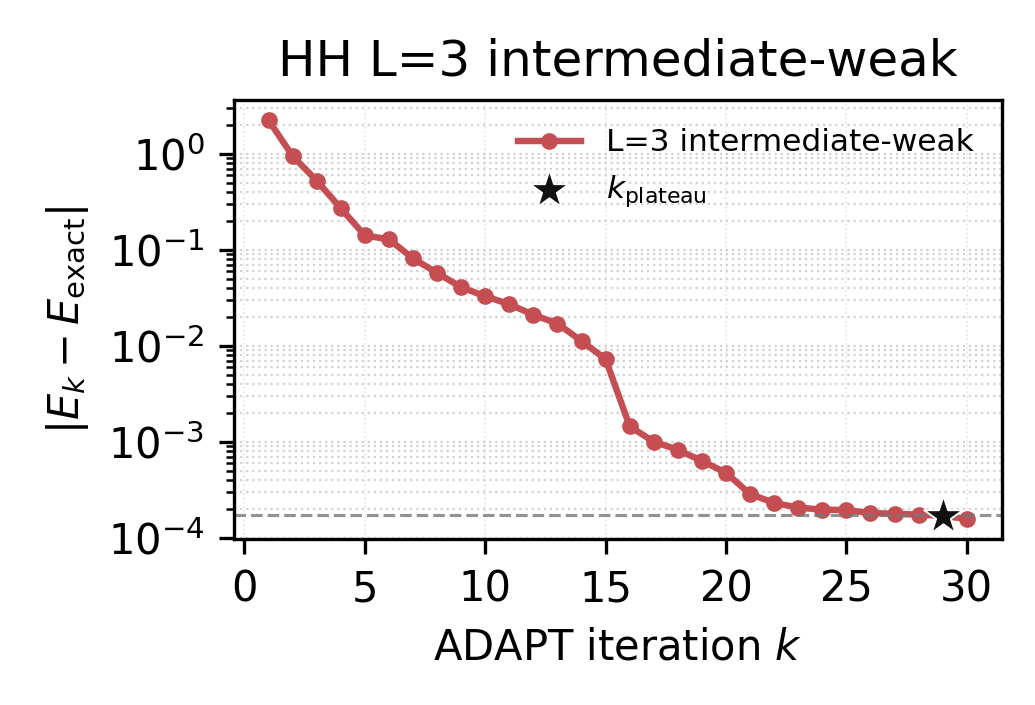
\includegraphics[width=\columnwidth]{figures/paper_i_hh_l3_intermediate_weak_physical_lanes_support_20260709/paper_i_hh_l3_intermediate_weak_error_vs_iteration_20260709.pdf}
\captionof{figure}{Three-site intermediate--weak Hubbard--Holstein SNAKE error versus ADAPT iteration for the physical-lane operator pool. The marker indicates the inferred plateau prefix \(k_{\rm pl}=29\).}
\label{fig:hh_l3_intermediate_weak_error_vs_iteration}
\end{center}

\begin{center}
\captionof{table}{\label{tab:hh_l3_intermediate_weak_plateau_costs}Three-site intermediate--weak Hubbard--Holstein SNAKE plateau-prefix Qiskit costs.}
\begin{tabular}{lrrrrrr}
\toprule
Method & \(k_{\rm pl}\) & \(|\Delta E|\) & \(N_{\twq}\) & \(D_{\twq}\) & \(D_c\) & \(S\) \\
\midrule
SNAKE & 29 & \(1.689\times10^{-4}\) & 122 & 98 & 488 & 44{,}467 \\
\bottomrule
\end{tabular}
\end{center}


\section{Spin-boson/Rabi benchmark}
\label{app:spin_boson_rabi}

The finite-mode spin-boson/Rabi benchmark is
\begin{equation*}
\begin{aligned}
H_{\rm SB}
&=-t_s\sigma_x+\Delta\sigma_z+\omega_0 b^\dagger b
+u_xX_b\sigma_x+g_zX_b\sigma_z,\\
X_b&=b^\dagger+b .
\end{aligned}
% source label: eq:spin_boson_rabi_appendix
\end{equation*}
Here \(\sigma_x,\sigma_y,\sigma_z\) are the Pauli matrices acting on the
two-level subsystem, and \(b^\dagger,b\) are truncated mode creation and
annihilation operators. The coefficient \(t_s\) sets the transverse two-level
term, \(\Delta\) is the longitudinal bias, \(\omega_0\) is the boson frequency,
and \(u_x\) and \(g_z\) are transverse and longitudinal quadrature-coupling
strengths. The conventional ultrastrong threshold is near
\(g/\omega_0\simeq 0.1\); the displayed rows use \(u_x=0\) and
\(g_z/\omega_0=0.05\) or \(0.1\) for the weak and stronger threshold-scale
points, respectively, with boson occupation cutoffs \(n_b^{\max}=1\) and
\(n_b^{\max}=2\) \cite{Kockum2019Ultrastrong,FornDiaz2019Ultrastrong}.

For the spin-boson/Rabi Hamiltonian, the operator pool combines two-level-system
rotations, bosonic quadrature response, nonlinear bosonic relaxation,
spin-conditioned bosonic response, and Hamiltonian-block channels. With
\(P_b=\ii(b^\dagger-b)\) and \(n_b=b^\dagger b\), the pool includes spin-only
channels, pure bosonic channels built from \(X_b\), \(P_b\), and \(n_b\),
spin-conditioned transverse channels such as \(X_b\sigma_x\), \(P_b\sigma_x\),
and \(n_b\sigma_x\), spin-conditioned longitudinal channels such as
\(X_b\sigma_z\), \(P_b\sigma_z\), and \(n_b\sigma_z\), nonlinear bosonic
channels such as \(\{n_b,P_b\}=n_bP_b+P_bn_b\) and \(X_bP_b+P_bX_b\), and
Hamiltonian-block channels. For the stronger cutoff case, the pool also
includes \(\sigma_y\)-conditioned correlation channels. SNAKE shortlists these
candidates through physical operator-type lanes separating two-level-system
motion, linear boson response, nonlinear boson response, transverse coupling,
longitudinal coupling, and Hamiltonian-block motion.

\noindent\begin{minipage}{0.49\columnwidth}
\begin{center}
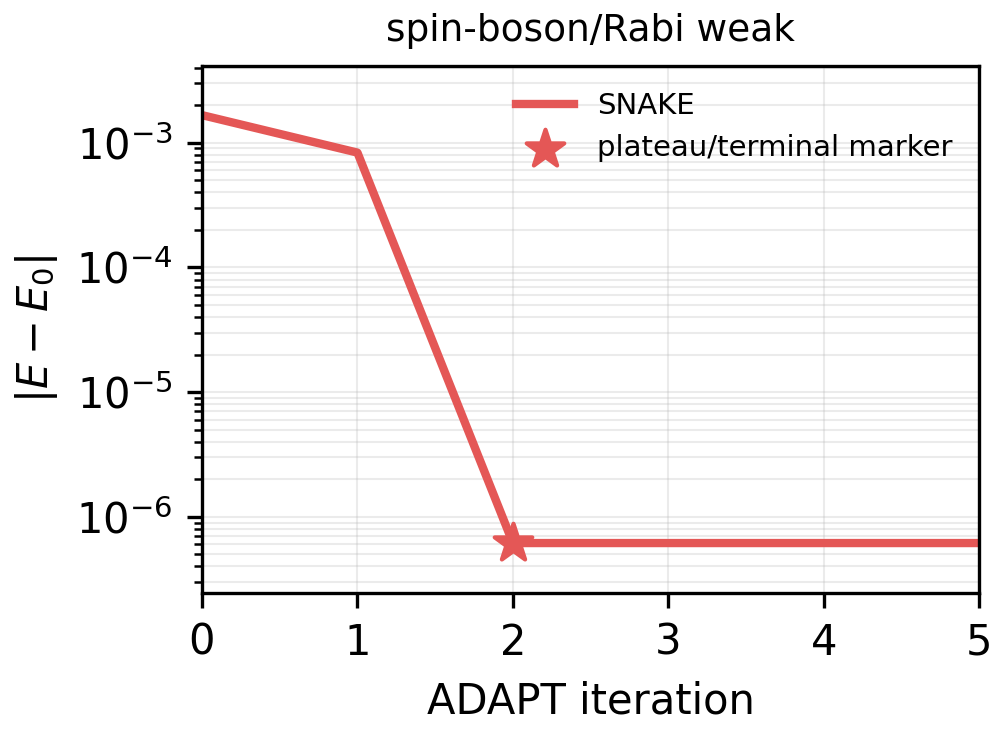
\includegraphics[width=\columnwidth]{figures/paper_i_alt_hamiltonian_1p75_20260709/paper_i_alt_snake_spin_boson_weak_error_vs_iteration.pdf}
\par\smallskip
\scriptsize
\textit{weak spin-boson/Rabi}
\par\smallskip
\setlength{\tabcolsep}{1.2pt}
\resizebox{\columnwidth}{!}{%
\begin{tabular}{@{}cccccc@{}}
\toprule
$k_{\rm pl}$ & $|\Delta E|$ & $N_{\twq}$ & $D_{\twq}$ & $D_c$ & $S$ \\
\midrule
2 & \(6{\times}10^{-7}\) & 19 & 17 & 123 & 685 \\
\bottomrule
\end{tabular}
}
\end{center}
\end{minipage}\hfill
\begin{minipage}{0.49\columnwidth}
\begin{center}
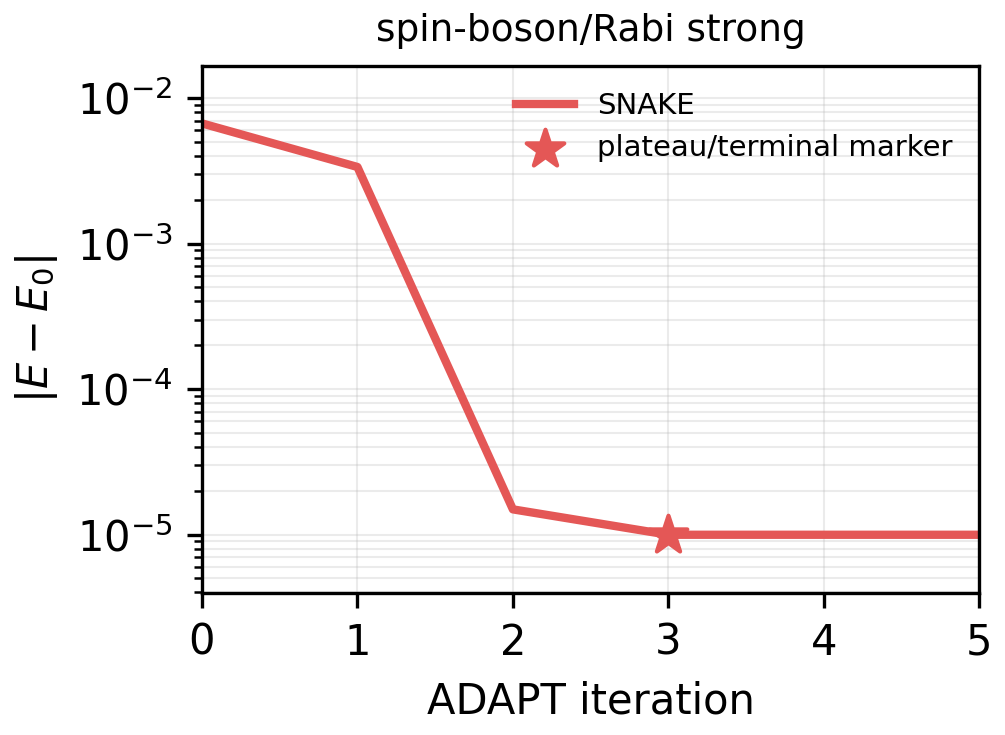
\includegraphics[width=\columnwidth]{figures/paper_i_alt_hamiltonian_1p75_20260709/paper_i_alt_snake_spin_boson_strong_error_vs_iteration.pdf}
\par\smallskip
\scriptsize
\textit{strong spin-boson/Rabi}
\par\smallskip
\setlength{\tabcolsep}{1.2pt}
\resizebox{\columnwidth}{!}{%
\begin{tabular}{@{}cccccc@{}}
\toprule
$k_{\rm pl}$ & $|\Delta E|$ & $N_{\twq}$ & $D_{\twq}$ & $D_c$ & $S$ \\
\midrule
3 & \(10{\times}10^{-6}\) & 115 & 111 & 723 & 3{,}754 \\
\bottomrule
\end{tabular}
}
\end{center}
\end{minipage}
\captionof{figure}{Spin-boson/Rabi SNAKE error versus ADAPT iteration and Qiskit plateau-prefix costs for weak and strong coupling.}
\par\addvspace{1.0ex}

\section{Bose--Hubbard benchmark}
\label{app:bose_hubbard}

For the Bose--Hubbard Hamiltonian, let \(b_i^\dagger,b_i\) be the bosonic
creation and annihilation operators on site \(i\). We define the local number
and quadrature operators
\[
n_i=b_i^\dagger b_i,\qquad
x_i=b_i+b_i^\dagger,\qquad
p_i=\ii(b_i^\dagger-b_i).
\]
The two-site open-boundary benchmark Hamiltonian is
\begin{equation*}
\begin{aligned}
H_{\rm BH}
&=-t\sum_{\langle i,j\rangle}
(b_i^\dagger b_j+b_j^\dagger b_i)
+\omega_0\sum_i n_i\\
&\quad+\frac{U_b}{2}\sum_i n_i(n_i-I)
+\Delta_v\sum_i(-1)^i n_i .
\end{aligned}
% source label: eq:bose_hubbard_appendix
\end{equation*}
Here \(t\) is the nearest-neighbor hopping amplitude, \(\omega_0\) is the
onsite boson energy, \(U_b\) is the onsite boson--boson interaction,
\(\Delta_v\) is the staggered onsite potential, \(I\) is the local identity,
and \(\langle i,j\rangle\) denotes nearest-neighbor sites. The displayed rows
use \(t=1\), \(\omega_0=1\), \(\Delta_v=0.25\), binary encoding with local
boson occupation cutoff \(n_b^{\max}=2\), and \(U_b=2\) or \(U_b=6\) for the
weak and strong interaction rows, respectively.
The operator pool is partitioned into physical operator-type lanes for number
and density interactions, onsite quadrature response, intersite quadrature
response, single-particle hopping/current, density-assisted transport, pair
transport, and Hamiltonian-block channels. These lanes include onsite number
operators \(n_i\), nonlinear number terms \(n_i^2\) and \(n_in_j\), onsite
quadratures \(x_i\), \(p_i\), \(x_i^2\), and \(p_i^2\), intersite quadratures
\(x_ix_j\) and \(p_ip_j\), hopping/current generators between sites,
density-weighted hopping/current generators, pair-hop/current generators, and
grouped Bose--Hubbard Hamiltonian blocks.

\noindent\begin{minipage}{0.49\columnwidth}
\begin{center}
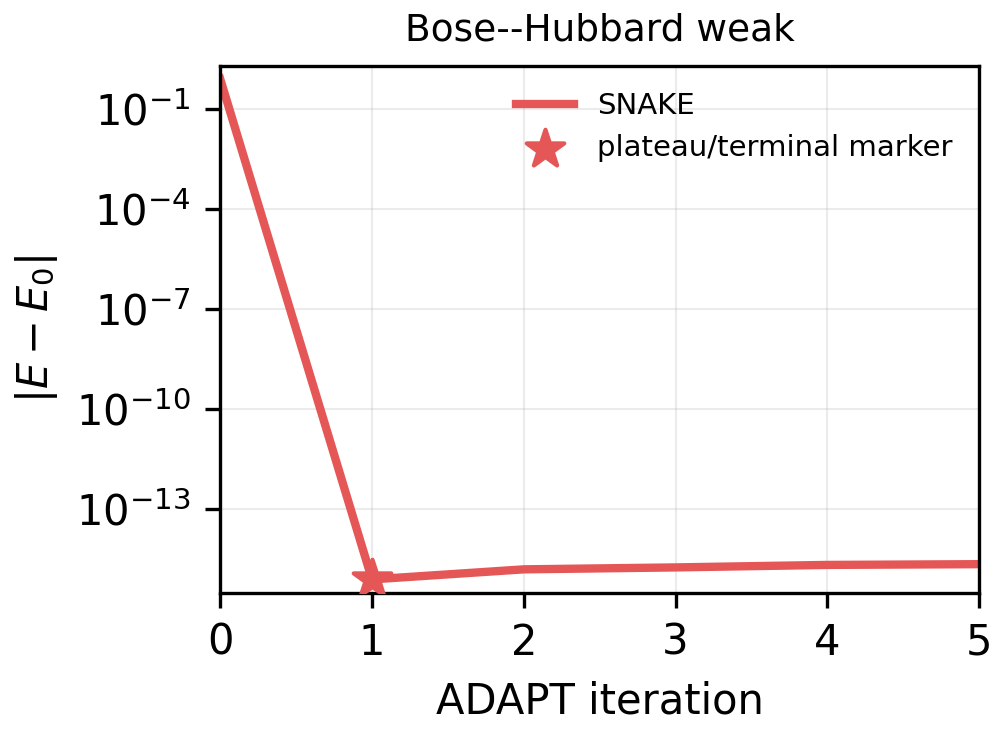
\includegraphics[width=\columnwidth]{figures/paper_i_alt_hamiltonian_1p75_20260709/paper_i_alt_snake_bose_hubbard_weak_error_vs_iteration.pdf}
\par\smallskip
\scriptsize
\textit{weak Bose--Hubbard}
\par\smallskip
\setlength{\tabcolsep}{1.2pt}
\resizebox{\columnwidth}{!}{%
\begin{tabular}{@{}cccccc@{}}
\toprule
$k_{\rm pl}$ & $|\Delta E|$ & $N_{\twq}$ & $D_{\twq}$ & $D_c$ & $S$ \\
\midrule
1 & \(8{\times}10^{-16}\) & 160 & 160 & 870 & 1{,}799 \\
\bottomrule
\end{tabular}
}
\end{center}
\end{minipage}\hfill
\begin{minipage}{0.49\columnwidth}
\begin{center}
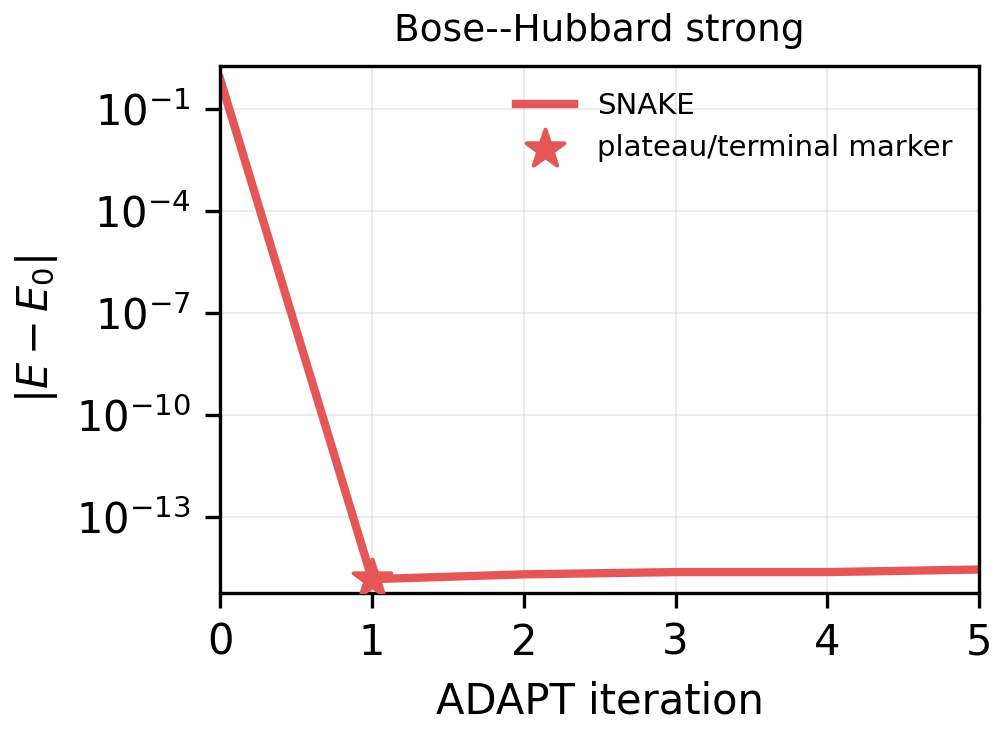
\includegraphics[width=\columnwidth]{figures/paper_i_alt_hamiltonian_1p75_20260709/paper_i_alt_snake_bose_hubbard_strong_error_vs_iteration.pdf}
\par\smallskip
\scriptsize
\textit{strong Bose--Hubbard}
\par\smallskip
\setlength{\tabcolsep}{1.2pt}
\resizebox{\columnwidth}{!}{%
\begin{tabular}{@{}cccccc@{}}
\toprule
$k_{\rm pl}$ & $|\Delta E|$ & $N_{\twq}$ & $D_{\twq}$ & $D_c$ & $S$ \\
\midrule
1 & \(1{\times}10^{-15}\) & 160 & 160 & 870 & 1{,}830 \\
\bottomrule
\end{tabular}
}
\end{center}
\end{minipage}
\captionof{figure}{Bose--Hubbard SNAKE error versus ADAPT iteration and Qiskit plateau-prefix costs for weak and strong interaction.}
\par\addvspace{1.0ex}

\section{Hubbard benchmarks}
\label{app:supplementary_transfer_benchmarks}

The Hubbard benchmark Hamiltonian is
\begin{equation*}
H_{\rm Hub}
=-t\sum_{\langle i,j\rangle,\sigma}
(c_{i\sigma}^{\dagger}c_{j\sigma}+c_{j\sigma}^{\dagger}c_{i\sigma})
+U\sum_i n_{i\uparrow}n_{i\downarrow}.
% source label: eq:hubbard_appendix
\end{equation*}
Here \(c_{i\sigma}^{\dagger},c_{i\sigma}\) are fermionic creation and
annihilation operators, \(n_{i\sigma}=c_{i\sigma}^{\dagger}c_{i\sigma}\),
\(\sigma\in\{\uparrow,\downarrow\}\), \(t\) is the nearest-neighbor hopping
amplitude, \(U\) is the onsite Hubbard interaction, and
\(\langle i,j\rangle\) denotes nearest-neighbor sites.
The displayed rows use a two-site open chain at half filling with \(t=1\).
For the Hubbard chain, the weak-coupling limit is given by
\(U/t\ll 1\), with correlation strength increasing as \(U/t\) grows;
we use \(U/t=0.25\) as a weak regime representative and \(U/t=8\) as the
strong-correlation point \cite{Arovas2022Hubbard}.

\noindent\begin{minipage}{0.49\columnwidth}
\begin{center}
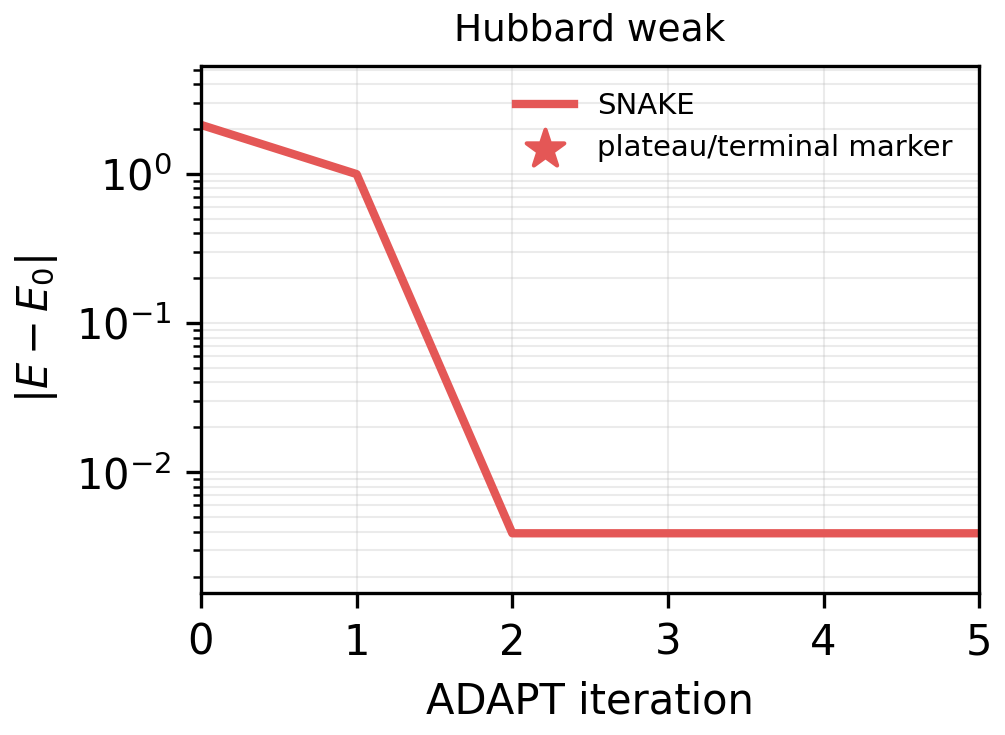
\includegraphics[width=\columnwidth]{figures/paper_i_alt_hamiltonian_1p75_20260709/paper_i_alt_snake_hubbard_weak_error_vs_iteration.pdf}
\par\smallskip
\scriptsize
\textit{weak Hubbard}
\par\smallskip
\setlength{\tabcolsep}{1.2pt}
\resizebox{\columnwidth}{!}{%
\begin{tabular}{@{}cccccc@{}}
\toprule
$k_{\rm pl}$ & $|\Delta E|$ & $N_{\twq}$ & $D_{\twq}$ & $D_c$ & $S$ \\
\midrule
8 & \(2{\times}10^{-11}\) & 18 & 10 & 120 & 5{,}936 \\
\bottomrule
\end{tabular}
}
\end{center}
\end{minipage}\hfill
\begin{minipage}{0.49\columnwidth}
\begin{center}
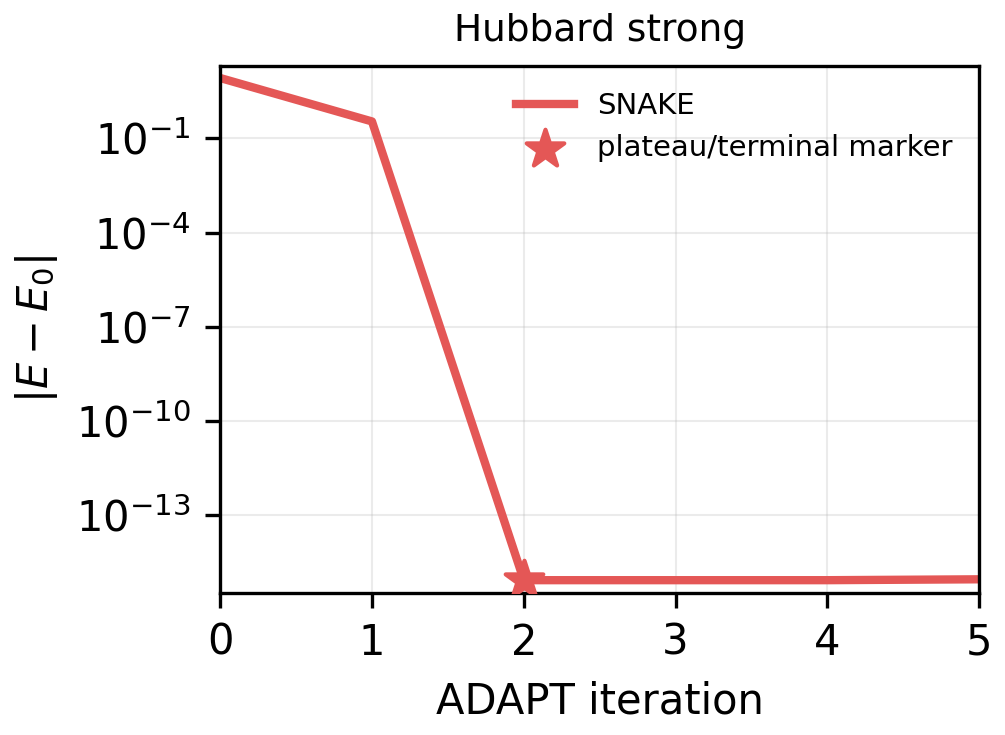
\includegraphics[width=\columnwidth]{figures/paper_i_alt_hamiltonian_1p75_20260709/paper_i_alt_snake_hubbard_strong_error_vs_iteration.pdf}
\par\smallskip
\scriptsize
\textit{strong Hubbard}
\par\smallskip
\setlength{\tabcolsep}{1.2pt}
\resizebox{\columnwidth}{!}{%
\begin{tabular}{@{}cccccc@{}}
\toprule
$k_{\rm pl}$ & $|\Delta E|$ & $N_{\twq}$ & $D_{\twq}$ & $D_c$ & $S$ \\
\midrule
2 & \(8{\times}10^{-16}\) & 52 & 52 & 274 & 751 \\
\bottomrule
\end{tabular}
}
\end{center}
\end{minipage}
\captionof{figure}{Hubbard SNAKE error versus ADAPT iteration and Qiskit plateau-prefix costs for weak and strong interaction.}
\par\addvspace{1.0ex}

\section{SPSA optimizer settings and sensitivity}
\label{app:spsa_settings}

SPSA-based diagnostic and comparator records use simultaneous perturbation
stochastic approximation as the inner optimizer
\cite{Spall1992SPSA,Kandala2017}. This optimizer appendix is separated from
the SNAKE algorithmic settings because SPSA is an inner-refit convention, not a
shortlisting, batching, insertion, or ablation rule.

At SPSA optimizer step \(m\), with Rademacher perturbation vector
\(\Delta_m\), the two-evaluation gradient estimator and parameter update are
\begin{align*}
a_m&=\frac{a}{(A+m+1)^\alpha},\qquad
c_m=\frac{c}{(m+1)^\gamma}, \nonumber\\
E_m^\pm&=E(\boldsymbol{\theta}_m\pm c_m\Delta_m), \nonumber\\
(\widehat g_m)_i&=\frac{E_m^+-E_m^-}{2c_m(\Delta_m)_i}, \nonumber\\
\boldsymbol{\theta}_{m+1}&=\boldsymbol{\theta}_m-a_m\widehat{\mathbf g}_m .
% source label: eq:spsa_inner_optimizer
\end{align*}
The schedule family uses \(m_{\max}=200\) unless a diagnostic row states a
larger budget. The realized Hubbard--Holstein schedule parameters are as
follows; ranges denote the minimum and maximum over the six regimes.
\begin{center}
\scriptsize
\setlength{\tabcolsep}{1.4pt}
\renewcommand{\arraystretch}{1.05}
\begin{tabular}{lcccccc}
Method & \(m_{\max}\) & \(a\) & \(c\) & \(A\) & \(\alpha\) & \(\gamma\)\\
Append & 200 & 0.0195--0.0454 & 0.00502--0.0118 & 12.4--59.0 & 0.602 & 0.101\\
Geo & 200 & 0.0169--0.0741 & 0.00501--0.0368 & 13.2--86.5 & 0.602 & 0.101\\
SNAKE & 200 & 0.100 & 0.020 & 5.0 & 0.602 & 0.101\\
\end{tabular}
\end{center}

\clearpage
\begin{thebibliography}{99}

\bibitem{Hubbard1963}
J. Hubbard,
``Electron correlations in narrow energy bands,''
\emph{Proceedings of the Royal Society of London A} \textbf{276}, 238 (1963).

\bibitem{Holstein1959a}
T. Holstein,
``Studies of polaron motion: Part I. The molecular-crystal model,''
\emph{Annals of Physics} \textbf{8}, 325 (1959).

\bibitem{Holstein1959b}
T. Holstein,
``Studies of polaron motion: Part II. The small polaron,''
\emph{Annals of Physics} \textbf{8}, 343 (1959).

\bibitem{Sakkinen2015HolsteinDimer}
N. S\"akkinen, Y. Peng, H. Appel, and R. van Leeuwen,
``Many-body Green's function theory for electron-phonon interactions: Ground state properties of the Holstein dimer,''
\emph{Journal of Chemical Physics} \textbf{143}, 234101 (2015).

\bibitem{Dorfner2015HolsteinDecay}
F. Dorfner, L. Vidmar, C. Brockt, E. Jeckelmann, and F. Heidrich-Meisner,
``Real-time decay of a highly excited charge carrier in the one-dimensional Holstein model,''
\emph{Physical Review B} \textbf{91}, 104302 (2015).

\bibitem{tenBrink2022HolsteinDynamics}
M. ten Brink, S. Gr\"aber, M. Hopjan, D. Jansen, J. Stolpp, F. Heidrich-Meisner, and P.~E. Bl\"ochl,
``Real-time non-adiabatic dynamics in the one-dimensional Holstein model: Trajectory-based vs exact methods,''
\emph{Journal of Chemical Physics} \textbf{156}, 234109 (2022).

\bibitem{Cataudella1999HolsteinVariational}
V. Cataudella, G. De Filippis, and G. Iadonisi,
``A new variational approach for the Holstein molecular-crystal model,''
\emph{Physical Review B} \textbf{60}, 15163 (1999).

\bibitem{ClayHardikar2005HH}
R.~T. Clay and R.~P. Hardikar,
``Intermediate phase of the one-dimensional half-filled Hubbard-Holstein model,''
\emph{Physical Review Letters} \textbf{95}, 096401 (2005).

\bibitem{Tezuka2007HH}
A. Tezuka, R. Arita, and H. Aoki,
``Phase diagram for the one-dimensional Hubbard-Holstein model: a density-matrix renormalization group study,''
\emph{Physical Review B} \textbf{76}, 155114 (2007).

\bibitem{Weisse2008}
A. Wei{\ss}e and H. Fehske,
``Exact diagonalization techniques,''
in \emph{Computational Many-Particle Physics},
edited by H. Fehske, R. Schneider, and A. Wei{\ss}e,
Lecture Notes in Physics Vol. 739 (Springer, Berlin, Heidelberg, 2008), pp. 529--544.

\bibitem{Troyer2005}
M. Troyer and U.-J. Wiese,
``Computational complexity and fundamental limitations to fermionic quantum Monte Carlo simulations,''
\emph{Physical Review Letters} \textbf{94}, 170201 (2005).

\bibitem{Schollwock2011}
U. Schollw\"ock,
``The density-matrix renormalization group in the age of matrix product states,''
\emph{Annals of Physics} \textbf{326}, 96 (2011).

\bibitem{Arovas2022Hubbard}
D.~P. Arovas, E. Berg, S.~A. Kivelson, and S. Raghu,
``The Hubbard model,''
\emph{Annual Review of Condensed Matter Physics} \textbf{13}, 239--274 (2022).

\bibitem{LeBlanc2015HubbardBenchmarks}
J.~P.~F. LeBlanc et al.,
``Solutions of the two-dimensional Hubbard model: Benchmarks and results from a wide range of numerical algorithms,''
\emph{Physical Review X} \textbf{5}, 041041 (2015).

\bibitem{Qin2016AFQMCHubbard}
M. Qin, H. Shi, and S. Zhang,
``Benchmark study of the two-dimensional Hubbard model with auxiliary-field quantum Monte Carlo method,''
\emph{Physical Review B} \textbf{94}, 085103 (2016).

\bibitem{Alvertis2025HubbardVQE}
A.~M. Alvertis, A. Khan, T. Iadecola, P.~P. Orth, and N.~M. Tubman,
``Classical Benchmarks for Variational Quantum Eigensolver Simulations of the Hubbard Model,''
\emph{Quantum} \textbf{9}, 1748 (2025).

\bibitem{Lloyd1996}
S. Lloyd,
``Universal quantum simulators,''
\emph{Science} \textbf{273}, 1073--1078 (1996).

\bibitem{AspuruGuzik2005}
A. Aspuru-Guzik, A.~D. Dutoi, P.~J. Love, and M. Head-Gordon,
``Simulated quantum computation of molecular energies,''
\emph{Science} \textbf{309}, 1704--1707 (2005).

\bibitem{Preskill2018NISQ}
J. Preskill,
``Quantum computing in the NISQ era and beyond,''
\emph{Quantum} \textbf{2}, 79 (2018).

\bibitem{Huggins2021Measurements}
W.~J. Huggins, J.~R. McClean, N.~C. Rubin, Z. Jiang, N. Wiebe, K.~B. Whaley, and R. Babbush,
``Efficient and noise resilient measurements for quantum chemistry on near-term quantum computers,''
\emph{npj Quantum Information} \textbf{7}, 23 (2021).

\bibitem{Romero2018UCC}
J. Romero, R. Babbush, J.~R. McClean, C. Hempel, P.~J. Love, and A. Aspuru-Guzik,
``Strategies for quantum computing molecular energies using the unitary coupled cluster ansatz,''
\emph{Quantum Science and Technology} \textbf{4}, 014008 (2018).

\bibitem{Peruzzo2014}
A. Peruzzo, J. McClean, P. Shadbolt, M.-H. Yung, X.-Q. Zhou, P.~J. Love, A. Aspuru-Guzik, and J.~L. O'Brien,
``A variational eigenvalue solver on a photonic quantum processor,''
\emph{Nature Communications} \textbf{5}, 4213 (2014).

\bibitem{McClean2016}
J.~R. McClean, J. Romero, R. Babbush, and A. Aspuru-Guzik,
``The theory of variational hybrid quantum-classical algorithms,''
\emph{New Journal of Physics} \textbf{18}, 023023 (2016).

\bibitem{Kandala2017}
A. Kandala, A. Mezzacapo, K. Temme, M. Takita, M. Brink, J.~M. Chow, and J.~M. Gambetta,
``Hardware-efficient variational quantum eigensolver for small molecules and quantum magnets,''
\emph{Nature} \textbf{549}, 242 (2017).

\bibitem{Cerezo2021VQA}
M. Cerezo, A. Arrasmith, R. Babbush, S.~C. Benjamin, S. Endo, K. Fujii, J.~R. McClean, K. Mitarai, X. Yuan, L. Cincio, and P.~J. Coles,
``Variational quantum algorithms,''
\emph{Nature Reviews Physics} \textbf{3}, 625--644 (2021).

\bibitem{VanStraaten2021MeasurementCost}
B. van Straaten and B. Koczor,
``Measurement cost of metric-aware variational quantum algorithms,''
\emph{PRX Quantum} \textbf{2}, 030324 (2021).

\bibitem{Spall1992SPSA}
J.~C. Spall,
``Multivariate stochastic approximation using a simultaneous perturbation gradient approximation,''
\emph{IEEE Transactions on Automatic Control} \textbf{37}, 332--341 (1992).

\bibitem{BonetMonroig2023Optimizer}
X. Bonet-Monroig, H. Wang, D. Vermetten, B. Senjean, C. Moussa, T. B\"ack, V. Dunjko, and T.~E. O'Brien,
``Performance comparison of optimization methods on variational quantum algorithms,''
\emph{Physical Review A} \textbf{107}, 032407 (2023).

\bibitem{Singh2023Optimizers}
H. Singh, S. Mishra, and S. Majumder,
``Benchmarking of different optimizers in the variational quantum algorithms for applications in quantum chemistry,''
\emph{Journal of Chemical Physics} \textbf{159}, 044117 (2023).

\bibitem{Jones2025FermiHubbardOptimizers}
B.~D.~M. Jones, L. Mineh, and A. Montanaro,
``Benchmarking a wide range of optimisers for solving the Fermi-Hubbard model using the variational quantum eigensolver,''
\emph{arXiv:2411.13742} (2025).

\bibitem{McClean2018BarrenPlateaus}
J.~R. McClean, S. Boixo, V.~N. Smelyanskiy, R. Babbush, and H. Neven,
``Barren plateaus in quantum neural network training landscapes,''
\emph{Nature Communications} \textbf{9}, 4812 (2018).

\bibitem{LiBenjamin2017VQS}
Y. Li and S.~C. Benjamin,
``Efficient variational quantum simulator incorporating active error minimization,''
\emph{Physical Review X} \textbf{7}, 021050 (2017).

\bibitem{Yuan2019VQS}
X. Yuan, S. Endo, Q. Zhao, Y. Li, and S.~C. Benjamin,
``Theory of variational quantum simulation,''
\emph{Quantum} \textbf{3}, 191 (2019).

\bibitem{McClean2017QSE}
J.~R. McClean, M.~E. Kimchi-Schwartz, J. Carter, and W.~A. de Jong,
``Hybrid quantum-classical hierarchy for mitigation of decoherence and determination of excited states,''
\emph{Physical Review A} \textbf{95}, 042308 (2017).

\bibitem{Grimsley2019}
H.~R. Grimsley, S.~E. Economou, E. Barnes, and N.~J. Mayhall,
``An adaptive variational algorithm for exact molecular simulations on a quantum computer,''
\emph{Nature Communications} \textbf{10}, 3007 (2019).

\bibitem{Grimsley2023ADAPT}
H.~R. Grimsley, G.~S. Barron, E. Barnes, S.~E. Economou, and N.~J. Mayhall,
``Adaptive, problem-tailored variational quantum eigensolver mitigates rough parameter landscapes and barren plateaus,''
\emph{npj Quantum Information} \textbf{9}, 19 (2023).

\bibitem{Tang2021}
H.~L. Tang, V.~O. Shkolnikov, G.~S. Barron, H.~R. Grimsley, N.~J. Mayhall, E. Barnes, and S.~E. Economou,
``Qubit-ADAPT-VQE: An adaptive algorithm for constructing hardware-efficient ans\"atze on a quantum processor,''
\emph{PRX Quantum} \textbf{2}, 020310 (2021).

\bibitem{Yordanov2021}
Y.~S. Yordanov, V. Armaos, C.~H.~W. Barnes, and D.~R.~M. Arvidsson-Shukur,
``Qubit-excitation-based adaptive variational quantum eigensolver,''
\emph{Communications Physics} \textbf{4}, 228 (2021).

\bibitem{Feniou2023}
C. Feniou, M. Hassan, D. Traor\'e, E. Giner, Y. Maday, and J.-P. Piquemal,
``Overlap-ADAPT-VQE: Practical quantum chemistry on quantum computers via overlap-guided compact ans\"atze,''
\emph{Communications Physics} \textbf{6}, 192 (2023).

\bibitem{Majland2024vADAPT}
M. Majland, P. Ettenhuber, N.~T. Zinner, and O. Christiansen,
``Vibrational ADAPT-VQE: Critical points lead to problematic convergence,''
\emph{Journal of Chemical Physics} \textbf{160}, 154109 (2024).

\bibitem{Anastasiou2024}
P.~G. Anastasiou, Y. Chen, N.~J. Mayhall, E. Barnes, and S.~E. Economou,
``TETRIS-ADAPT-VQE: An adaptive algorithm that yields shallower, denser circuit ans\"atze,''
\emph{Physical Review Research} \textbf{6}, 013254 (2024).

\bibitem{Ramoa2025}
M. Ram\^oa, P.~G. Anastasiou, L.~P. Santos, N.~J. Mayhall, E. Barnes, and S.~E. Economou,
``Reducing the resources required by ADAPT-VQE using coupled exchange operators and improved subroutines,''
\emph{npj Quantum Information} \textbf{11}, 86 (2025).

\bibitem{Ramoa2025HessianRecycling}
M. Ramoa et al.,
``Reducing measurement costs by recycling the Hessian in adaptive variational quantum algorithms,''
\emph{Quantum Science and Technology} \textbf{10}, 015031 (2025).

\bibitem{He2026ParamADAPT}
R. He, X. Hong, Q. Chai, J. Guan, J. Zhou, A. Ablimit, G. Cui, and S. Ying,
``Constructing Compact ADAPT Unitary Coupled-Cluster Ansatz with Parameter-Based Criterion,''
\emph{Journal of Chemical Theory and Computation} \textbf{22}, 5090--5101 (2026).

\bibitem{He2026HAADAPT}
R. He, C. Liu, X. Hong, Q. Chai, J. Zhou, J. Guan, G. Cui, and S. Ying,
``Hamiltonian-Aware ADAPT Variational Quantum Eigensolver for Molecular Ground-State Simulation,''
\emph{arXiv:2606.13118} (2026).

\bibitem{Bespalova2026KADAPT}
T.~A. Bespalova, O. Ladhari, and G. Masella,
``K-ADAPT-VQE: Optimizing Molecular Ground State Searches by Chunking Operators,''
in \emph{Quantum Engineering Sciences and Technologies for Industry and Services}, Communications in Computer and Information Science \textbf{2744}, 226--235 (Springer, Cham, 2026).

\bibitem{Nocedal2006TrustRegion}
J. Nocedal and S. J. Wright,
``Trust-Region Methods,''
in \emph{Numerical Optimization}, Springer (New York, NY, 1994).

\bibitem{IglewiczHoaglin1993}
B. Iglewicz and D.~C. Hoaglin,
\emph{How to Detect and Handle Outliers},
ASQC Basic References in Quality Control: Statistical Techniques, Vol.~16
(ASQC Quality Press, Milwaukee, WI, 1993).

\bibitem{Burbidge1988IHS}
J.~B. Burbidge, L. Magee, and A.~L. Robb,
``Alternative transformations to handle extreme values of the dependent variable,''
\emph{Journal of the American Statistical Association} \textbf{83}, 123--127 (1988).

\bibitem{Ikhtiarudin2025ShotEfficient}
A. Ikhtiarudin, G. K. Sunnardianto, F. Fathurrahman, M. K. Agusta, and H. Dipojono,
``Shot-Efficient ADAPT-VQE via Reused Pauli Measurements and Variance-Based Shot Allocation,''
\emph{arXiv:2507.16879} (2025).

\bibitem{Lowerre1976Beam}
B. T. Lowerre,
``The Harpy Speech Recognition System,''
Ph.D. thesis, Carnegie Mellon University (1976).

\bibitem{Sohail2026GeoADAPT}
M.~A. Sohail and T. Koike-Akino,
``Geo-ADAPT-VQE: Quantum Information Metric-Aware Circuit Optimization for Quantum Chemistry,''
\emph{arXiv:2603.10325} (2026).

\bibitem{Stadelmann2025GradientTroughs}
T. Stadelmann and others,
``Strategies for overcoming gradient troughs in the ADAPT-VQE algorithm,''
\emph{arXiv:2512.25004} (2025).

\bibitem{ProvostVallee1980}
J.-P. Provost and G. Vall\'ee,
``Riemannian structure on manifolds of quantum states,''
\emph{Communications in Mathematical Physics} \textbf{76}, 289 (1980).

\bibitem{Stokes2020QNG}
J. Stokes, J. Izaac, N. Killoran, and G. Carleo,
``Quantum natural gradient,''
\emph{Quantum} \textbf{4}, 269 (2020).

\bibitem{Haug2021Capacity}
T. Haug, K. Bharti, and M.~S. Kim,
``Capacity and quantum geometry of parametrized quantum circuits,''
\emph{PRX Quantum} \textbf{2}, 040309 (2021).

\bibitem{Gacon2021QNSPSA}
J. Gacon, C. Zoufal, G. Carleo, and S. Woerner,
``Simultaneous perturbation stochastic approximation of the quantum Fisher information,''
\emph{Quantum} \textbf{5}, 567 (2021).

\bibitem{JavadiAbhari2024Qiskit}
A. Javadi-Abhari, M. Treinish, K. Krsulich, C.~J. Wood, J. Lishman, J. Gacon, S. Martiel, P.~D. Nation, L.~S. Bishop, A.~W. Cross, B.~R. Johnson, and J.~M. Gambetta,
``Quantum computing with Qiskit,''
\emph{arXiv:2405.08810} (2024).

\bibitem{QiskitAlgorithmsAdaptVQE}
Qiskit Community,
``AdaptVQE,''
\emph{Qiskit Algorithms documentation}, \url{https://qiskit-community.github.io/qiskit-algorithms/stubs/qiskit_algorithms.AdaptVQE.html}.

\bibitem{Larocca2023Overparametrization}
M. Larocca, N. Ju, D. Garc{\'i}a-Mart{\'i}n, P.~J. Coles, and M. Cerezo,
``Theory of overparametrization in quantum neural networks,''
\emph{Nature Computational Science} \textbf{3}, 542--551 (2023).

\bibitem{Verteletskyi2020CliqueCover}
V. Verteletskyi, T.-C. Yen, and A.~F. Izmaylov,
``Measurement optimization in the variational quantum eigensolver using a minimum clique cover,''
\emph{Journal of Chemical Physics} \textbf{152}, 124114 (2020).

\bibitem{Yen2020CompatibleMeasurements}
T.-C. Yen, V. Verteletskyi, and A.~F. Izmaylov,
``Measuring all compatible operators in one series of single-qubit measurements using unitary transformations,''
\emph{Journal of Chemical Theory and Computation} \textbf{16}, 2400 (2020).


\bibitem{Macridin2018}
A. Macridin, P. Spentzouris, J. Amundson, and R. Harnik,
``Electron-phonon systems on a universal quantum computer,''
\emph{Physical Review Letters} \textbf{121}, 110504 (2018).

\bibitem{Sawaya2020}
N.~P.~D. Sawaya, T. Menke, T.~H. Kyaw, S. Johri, A. Aspuru-Guzik, and G.~G. Guerreschi,
``Resource-efficient digital quantum simulation of $d$-level systems for photonic, vibrational, and spin-$s$ Hamiltonians,''
\emph{npj Quantum Information} \textbf{6}, 49 (2020).

\bibitem{Li2023}
W. Li, J. Ren, S. Huai, T. Cai, Z. Shuai, and S. Zhang,
``Efficient quantum simulation of electron-phonon systems by variational basis state encoder,''
\emph{Physical Review Research} \textbf{5}, 023046 (2023).

\bibitem{Denner2023}
M.~M. Denner, H. Yan, N. A. Sinitsyn, and others,
``A hybrid quantum-classical method for electron-phonon systems,''
\emph{Communications Physics} \textbf{6}, 317 (2023).

\bibitem{Dutta2024BosonicChemistry}
R. Dutta et al.,
``Simulating chemistry on bosonic quantum devices,''
\emph{Journal of Chemical Theory and Computation} \textbf{20}, 6426--6441 (2024).

\bibitem{Dutta2026QumodeVQE}
R. Dutta, C. Cianci, A.~V. Soudackov, Y. Wang, C. Xu, D. Mazziotti, L.~F. Santos, and V.~S. Batista,
``Qumode-Based Variational Quantum Eigensolver for Molecular Excited States,''
\emph{Journal of Chemical Theory and Computation} \textbf{22}, 993--1003 (2026).

\bibitem{Rinaldi2022MatrixModels}
E. Rinaldi, X. Han, M. Hassan, Y. Feng, F. Nori, M. McGuigan, and M. Hanada,
``Matrix-Model Simulations Using Quantum Computing, Deep Learning, and Lattice Monte Carlo,''
\emph{PRX Quantum} \textbf{3}, 010324 (2022).

\bibitem{Dao2025SU2MatrixVQE}
H.~L. Dao,
``Exploring new variational quantum circuit ansatzes for solving SU(2) matrix models,''
\emph{European Physical Journal C} \textbf{85}, 705 (2025).

\bibitem{Peng2025BosonHamiltonians}
B. Peng, Y. Su, D. Claudino, K. Kowalski, G. H. Low, and M. Roetteler,
``Quantum simulation of boson-related Hamiltonians: Techniques, effective Hamiltonian construction, and error analysis,''
\emph{Quantum Science and Technology} \textbf{10}, 023002 (2025).

\bibitem{Kockum2019Ultrastrong}
A.~F. Kockum, A. Miranowicz, S. De Liberato, S. Savasta, and F. Nori,
``Ultrastrong coupling between light and matter,''
\emph{Nature Reviews Physics} \textbf{1}, 19--40 (2019).

\bibitem{FornDiaz2019Ultrastrong}
P. Forn-D{\'i}az, L. Lamata, E. Rico, J. Kono, and E. Solano,
``Ultrastrong coupling regimes of light-matter interaction,''
\emph{Reviews of Modern Physics} \textbf{91}, 025005 (2019).

\bibitem{Vaquero2025PrunedADAPT}
N. Vaquero-Sabater, A. Carreras, and D. Casanova,
``Pruned-ADAPT-VQE: Compacting Molecular Ans\"atze by Removing Irrelevant Operators,''
\emph{Journal of Chemical Theory and Computation} \textbf{21}, 8720--8728 (2025).

\end{thebibliography}

\end{document}
